\documentclass{article}

\usepackage{corl_2026}
\usepackage{amsmath}
\usepackage{amssymb}
\usepackage{booktabs}
\usepackage{graphicx}
\usepackage{tabularx}
\usepackage{algorithm}
\usepackage{algorithmic}
\usepackage{placeins}
\usepackage{enumitem}
\usepackage[table]{xcolor}
\definecolor{maroonprimary}{HTML}{8B1A2E}
\definecolor{maroonhl}{HTML}{FAE8EC}
\usepackage{float}
\usepackage{titlesec}
\titlespacing*{\section}{0pt}{2pt plus 1pt minus 1pt}{2pt plus 0pt minus 1pt}
\titlespacing*{\subsection}{0pt}{7pt plus 2pt minus 2pt}{2pt plus 1pt}
\titlespacing*{\subsubsection}{0pt}{4pt plus 2pt minus 1pt}{2pt}
\setlength{\floatsep}{3pt plus 1pt minus 1pt}
\setlength{\textfloatsep}{4pt plus 2pt minus 2pt}
\setlength{\intextsep}{4pt plus 2pt minus 1pt}
\setlength{\abovedisplayskip}{4pt plus 2pt minus 2pt}
\setlength{\belowdisplayskip}{4pt plus 2pt minus 2pt}
\setlength{\abovedisplayshortskip}{2pt plus 1pt}
\setlength{\belowdisplayshortskip}{3pt plus 1pt minus 1pt}

\newcommand{\methodsec}[1]{\noindent\textcolor{black}{\textbf{#1}}\enspace}

\title{Predictive Interoception for Embodied Autonomy: Preserving Future Action Capacity Before Collapse}

\author{Anonymous Authors}

\newcommand{\fac}{\mathrm{FAC}}
\newcommand{\obs}{o}
\newcommand{\act}{a}
\newcommand{\state}{s}
\newcommand{\ext}{x}
\newcommand{\body}{b}
\newcommand{\bodycost}{c^{\mathrm{body}}}
\newcommand{\task}{r^{\mathrm{task}}}
\newcommand{\collapse}{\mathcal{K}}
\newcommand{\E}{\mathbb{E}}
\newcommand{\ind}{\mathbb{I}}

\begin{document}
\maketitle

\begin{figure*}[h]
\centering
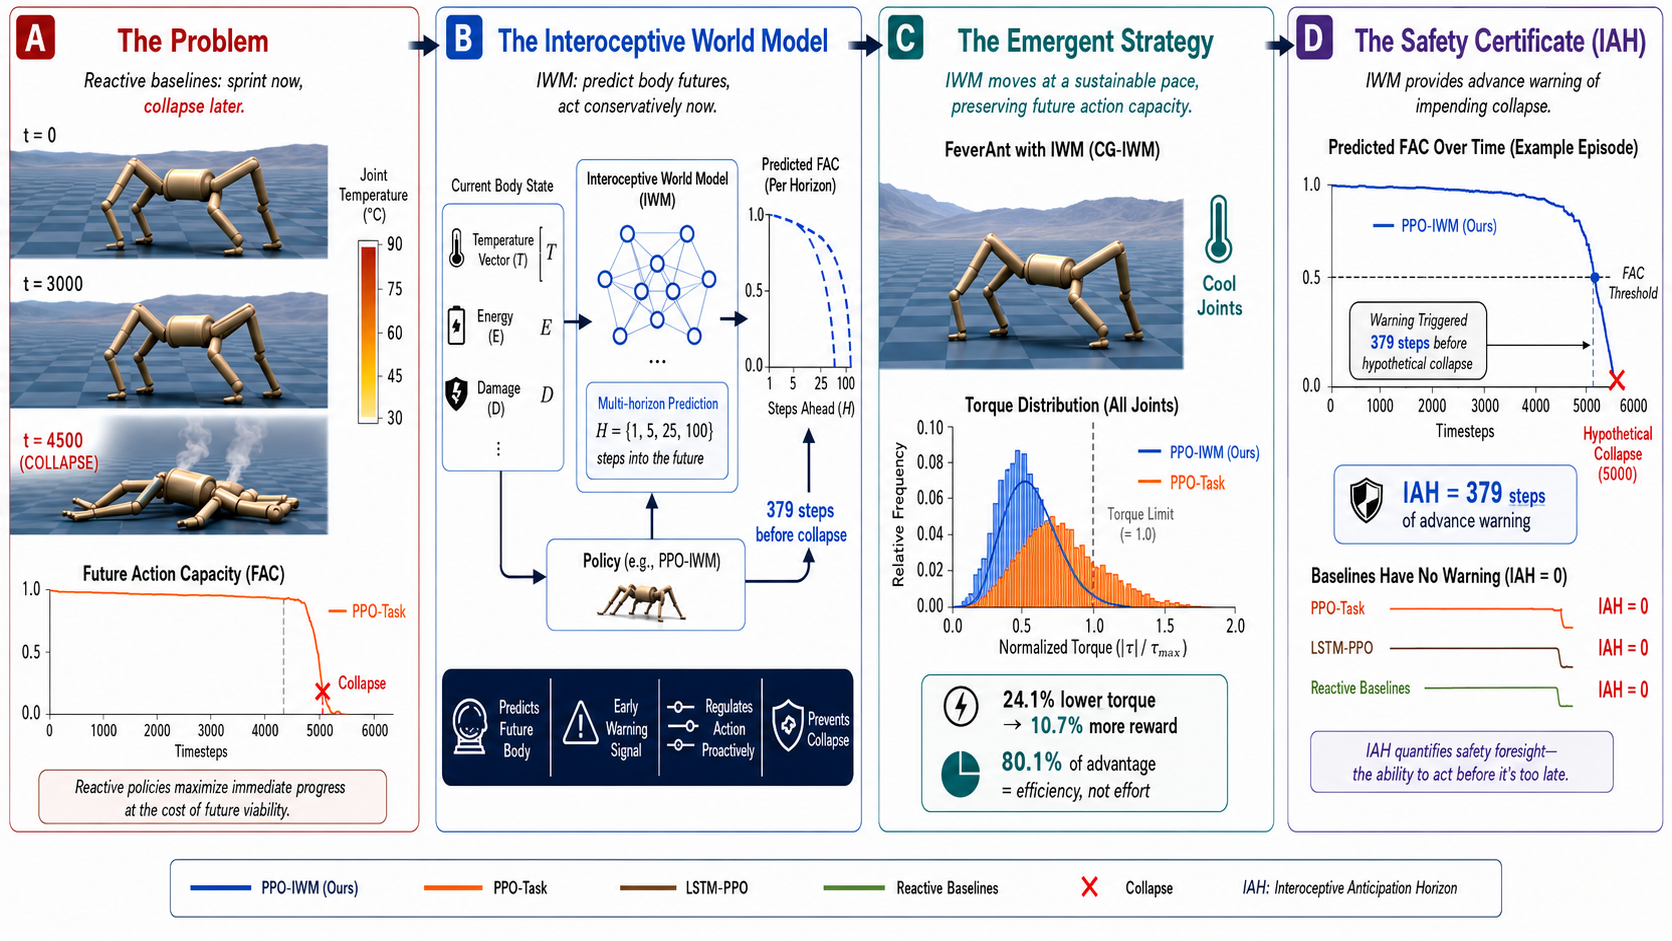
\includegraphics[width=0.99\linewidth]{figures/b_overview.png}
\caption{\textbf{Overview: problem, method, and results.}
A task-only agent depletes its body capacity (Future Action Capacity or FAC) through unconstrained actuator use and collapses, detectable only at the moment of failure.
The Interoceptive World Model (IWM) predicts future FAC loss across four horizons, shapes the policy preemptively, and achieves zero collapse, an average 379-step advance warning, and 10.7\% higher task reward, simultaneously, across all evaluated environments.}
\label{fig:story}
\end{figure*}


\begin{abstract}
Robots degrade not from external hazards but from their own actions: unconstrained actuator use overheats motors, compounds joint damage, and depletes energy reserves, collapsing the robot's ability to control itself in ways that are invisible until the moment of failure.
Existing safe-RL methods guard against external constraint violations; no prior method gives a robot a forward-looking signal of how far it is from losing the ability to act at all.

We introduce the \textbf{Interoceptive World Model (IWM)}: a neural predictor trained jointly with a control policy that forecasts how current actions will erode future control authority, shaping behavior preemptively rather than reacting to damage already done.
An \textbf{Adaptive IWM (AIWM)} extends this with online body-model personalization at deployment without policy retraining.

The most striking consequence is not safety but efficiency.
On BodyFutures-Bench --- four MuJoCo environments with latent body degradation dynamics --- IWM agents discover torque-efficient locomotion as an emergent property of self-preservation: the agent learns to be gentle with its joints not because gentleness is rewarded, but because overexertion destroys its future.
IWM simultaneously achieves zero collapse, higher task reward, and better body health --- strict Pareto-dominance with no efficiency objective --- while providing a deployable advance warning of impending incapacitation (Interoceptive Anticipation Horizon; IAH) absent from every reactive and memory-based baseline.
We release BodyFutures-Bench, all checkpoints, and IAH as a standard diagnostic for long-horizon robot health.
\end{abstract}

\keywords{robot body health, interoceptive world models, predictive safety, safe reinforcement learning, embodied autonomy}


\section{Introduction}

In real deployments, the body of a robot is a dynamical system subject to degradations from use. A locomotion policy that overheats actuators may leave the robot unable to move in the next episode; a manipulation policy exploiting high torques may degrade proprioception before the goal is reached. The action interface is, therefore, nonstationary: for instance, the same command at $t$ and $t+T$ can have different physical consequences because the robot's internal state has changed. Long-horizon robot learning requires agents that model not only the external world, but also the future of their own body - a policy cannot reliably preserve future control authority if it merely sees observable degradation through faults that can sometimes be catastrophic.

We introduce BodyFutures-Bench to characterize and quantify this challenge. The suite wraps standard MuJoCo tasks with latent body variables - energy, temperature, impact stress, wounds, damage, and sensor numbness - that affect future dynamics by weakening actuators, corrupting proprioception, and triggering collapse. Each environment logs a shared diagnostic contract (task reward, FAC, energy, damage, collapse) and exposes a ``sprinter vs.\ survivor'' tension: task-only policies deplete the body for short-horizon gain, while self-preserving policies should maintain future action capacity.

We address this with an \textbf{Interoceptive World Model (IWM)}: a neural predictor that learns which actions will erode the body's future ability to act, and uses that foresight to shape a policy that is simultaneously safer and more efficient. Rather than reacting to damage already done, the agent predicts it before it happens - and adjusts behavior accordingly. An \textbf{Adaptive IWM (AIWM)} extends this by updating its body model at deployment time, personalizing predictions to the specific robot at hand without any retraining of the control policy.

The experimental results yield a finding we did not anticipate: the agent does not merely survive longer --- it moves better.
Body-preservation shaping teaches torque efficiency as an emergent strategy, yielding simultaneous gains on task performance, body health, and collapse avoidance that no reactive baseline achieves, without any explicit efficiency objective.
The advance-warning capability --- quantified as IAH, the Interoceptive Anticipation Horizon --- transforms previously invisible degradation into an auditable, per-step safety signal that operators can query.
These three outcomes (efficiency, safety, and auditability) arise from a single architectural change: replacing reactive penalties with predictive body modeling.

This paper contributes: a deployable advance-warning metric (the Interoceptive Anticipation Horizon, IAH) showing that every reactive and recurrent baseline achieves zero warning while IWM fires hundreds of steps before incapacitation; strict Pareto-dominance across task performance, body health, and collapse avoidance replicated across four robot morphologies; a falsifiable observability criterion predicting exactly when interoceptive prediction helps and when it does not; BodyFutures-Bench with a shared diagnostic contract and all checkpoints publicly released; and online body-model personalization for deployment-time adaptation without policy retraining. A structured checklist with evidence pointers appears in Table~\ref{tab:contributions} (Appendix~\ref{app:contributions}).

\section{Related Work}
\label{sec:related}

\textbf{Safe RL.}~Constrained policy optimization~\citep{achiam2017constrained}, Safety Gym~\citep{ray2019safetygym}, Safety Gymnasium~\citep{ji2023safetygymnasium}, and SafeDreamer~\citep{huang2024safedreamer} address \emph{external} hazards via Lagrangian penalties. BodyFutures differs: the hazard is \emph{endogenous} (self-induced by the agent's own torques), its consequence is irreversible loss of future control authority (not a per-step constraint), and IWM's IAH quantifies \emph{how far before collapse} the predictor fires, a signal absent from all safe-RL approaches.

\textbf{World models.}~Dreamer~\citep{hafner2020dreamer,hafner2023dreamerv3}, TD-MPC2~\citep{hansen2023tdmpc2}, and MBPO~\citep{janner2019mbpo} predict \emph{external} state transitions. IWM instead predicts \emph{internal} body-state trajectories (future FAC, damage, energy) and AIWM updates the predictor online during deployment, personalising interoceptive predictions to the specific robot's degradation trajectory~\citep{seth2013interoceptive}, without retraining the policy.

\textbf{Self-modeling and adaptation.}~Bongard et al.~\citep{bongard2006resilient}, Cully et al.~\citep{cully2015robots}, RMA~\citep{kumar2021rma}, and actuator-network models~\citep{hwangbo2019learning} estimate or compensate for \emph{current} body parameters after damage; IWM predicts \emph{future} body trajectories and IAH measures how far in advance. AIWM borrows EWC~\citep{kirkpatrick2017overcoming} not for multi-task forgetting but for intra-episode online personalisation of interoceptive priors.

\textbf{Interoception and efficiency.}~Homeostatic RL~\citep{keramati2011homeostatic} and empowerment~\citep{klyubin2005empowerment} motivate FAC as retained future action authority. IWM discovers 24.1\% lower control cost as an emergent consequence of body-preservation shaping, not any explicit efficiency objective, breaking the stillness trap that defeats reactive energy penalties. See Appendix~\ref{app:relatedwork} for extended comparisons.

\section{Formal Problem}
\label{sec:problem}

A standard POMDP assumes a fixed action interface; body degradation violates this because overheated actuators, damaged joints, and depleted energy all change what the same command achieves at $t+T$ versus $t$.
We model self-preserving robot learning as an augmented POMDP.  The full state is $\state_t=(\ext_t,\body_t)$, where $\ext_t$ denotes external task state and $\body_t$ denotes latent body state such as actuator temperature, damage, energy, wounds, or sensor numbness.  The policy receives
\begin{equation}
    \obs_t = g(\ext_t,\tilde{\body}_t),
    \qquad
    \tilde{\body}_t \sim q(\tilde{\body}\mid \body_t),
\end{equation}
where $\tilde{\body}_t$ is absent, noisy, full, or indirect depending on the observation mode.  The transition couples external and internal dynamics:
\begin{equation}
    p(\state_{t+1}\mid \state_t,\act_t)
    =
    p(\ext_{t+1},\body_{t+1}\mid \ext_t,\body_t,\act_t).
\end{equation}
The task reward $\task_t$ measures external progress, while $\bodycost_t = c^{\mathrm{body}}(\body_t,\act_t)$ measures instantaneous internal degradation. Collapse is an event $\collapse_t \in \{0,1\}$ that terminates or marks failure when internal state leaves a viable region.

The central diagnostic is Future Action Capacity, $\fac(\body_t)\in[0,1]$.
FAC answers one question: if the robot had to execute its full behavioral repertoire right now, what fraction would still work?
A healthy robot can apply any torque; one with overheated actuators scaling commands to 30\% of nominal cannot.
FAC formalizes this as the effective fraction of the nominal action space:
\begin{equation}
    \fac(\body_t)
    \approx
    \frac{1}{|\mathcal{A}|}
    \int_{\mathcal{A}}
    \ind\left[Q_{\mathrm{act}}(\act,\body_t) \ge \tau_{\mathrm{eff}}\right] d\act,
\end{equation}
where $Q_{\mathrm{act}}$ is an environment-specific proxy for effective actuation and $\tau_{\mathrm{eff}}$ is a minimum useful-action quality threshold.  In implementation, FAC is a calibrated monotone scalar over energy, damage, temperature, stress, balance, and proprioceptive reliability.  It is not used as a hidden oracle for task success; it is logged as a body-preservation diagnostic and, for explicit viability baselines, used as a current penalty.

The standard task objective is
\begin{equation}
    J_{\mathrm{task}}(\pi)
    =
    \E_{\pi}\left[\sum_{t=0}^{T-1}\gamma^t \task_t\right].
\end{equation}
\section{BodyFutures-Bench}
\label{sec:benchmark}

BodyFutures-Bench augments standard MuJoCo tasks with internal degradation dynamics and a shared diagnostic contract.  Every environment step returns task reward, viability cost, FAC, energy, mean and maximum body stress signals, mean and maximum damage, true and noisy body state, collapse flag, and collapse reason.  Policies can be evaluated under four observation modes: no body observation, full body state, noisy interoception, and latent indirect signals. Reward modes include task-only, energy-regularized, current-viability, and IWM shaping.

\begin{table}[t]
\centering
\small
\caption{BodyFutures-Bench environments.  FeverAnt and WoundWalker are the primary CoRL claim environments; ThermalHopper and NumbArm are secondary tests used after stability and task-learning gates pass.}
\label{tab:envs}
\begin{tabularx}{\linewidth}{llX}
\toprule
Environment & Base task & Body dynamics and role \\
\midrule
FeverAnt & Ant-v5 & Primary locomotion task with multi-motor heat,
energy depletion, torque damage, actuator weakening, and overheating collapse. \\
WoundWalker & Walker2d-v5 & Primary locomotion task with wounds, balance
health, impact stress, energy depletion, asymmetric gait degradation, and collapse. \\
ThermalHopper & Hopper-v5 & Secondary locomotion stress test with landing
impact, thermal load, damage, energy, and actuator weakening. \\
NumbArm & Pusher-v5 & Secondary manipulation stress test with numbness,
proprioceptive corruption, manipulation load, damage, and energy depletion. \\
\bottomrule
\end{tabularx}
\end{table}

Each environment couples temperature-like stress, damage, and energy with action-driven nonlinear update rules; degradation feeds back into physics by scaling actuator commands, so a damaged body has reduced future ability to affect the environment. Full equations and environment-specific constants are in Appendix~\ref{app:envs} (Eqs.~\ref{eq:temp}--\ref{eq:scale}).

\section{Interoceptive World Models}
\label{sec:method}

{\textbf{Intuition.}
Three failure modes motivate the design:
(1)~\textbf{Reactive penalties fall into the stillness trap}: for $\lambda\|a\|^2$, $a\!=\!\mathbf{0}$ is a fixed point of the penalty gradient, freezing the agent rather than teaching efficient locomotion.
(2)~\textbf{Memory cannot anticipate depletion}: an LSTM encodes past torque history but cannot compute ``if I continue at this rate, my FAC will reach 0.1 in 100 steps'' --- the forward body gradient is absent by architecture.
(3)~\textbf{A body predictor provides that gradient}: it makes high-torque actions costly \emph{before} irreversible damage while leaving zero-torque states unpunished (healthy-state FAC is high at $a\!=\!\mathbf{0}$, so the task gradient dominates there).
An Interoceptive World Model (IWM) is a neural predictor of future body health trained jointly with the policy; for each transition it outputs predicted body state and future FAC at multiple horizons, giving the agent a window into how current behaviour will affect physical health many steps ahead:
\begin{equation}
    f_\theta(\obs_t,\act_t,\tilde{\body}_t)
    \rightarrow
    \left\{
    \hat{\body}_{t+1},
    \widehat{\fac}_{t,H},
    \hat c^{H}_{t},
    \hat p^{H}_{\mathrm{collapse},t}
    \right\}_{H\in\{1,5,25,100\}} .
\end{equation}
The final protocol uses an ensemble of bootstrapped predictors.  The ensemble is important because body-preservation penalties should be conservative when the model is uncertain in low-FAC or collapse-adjacent states.

\begin{figure*}[h]
\centering
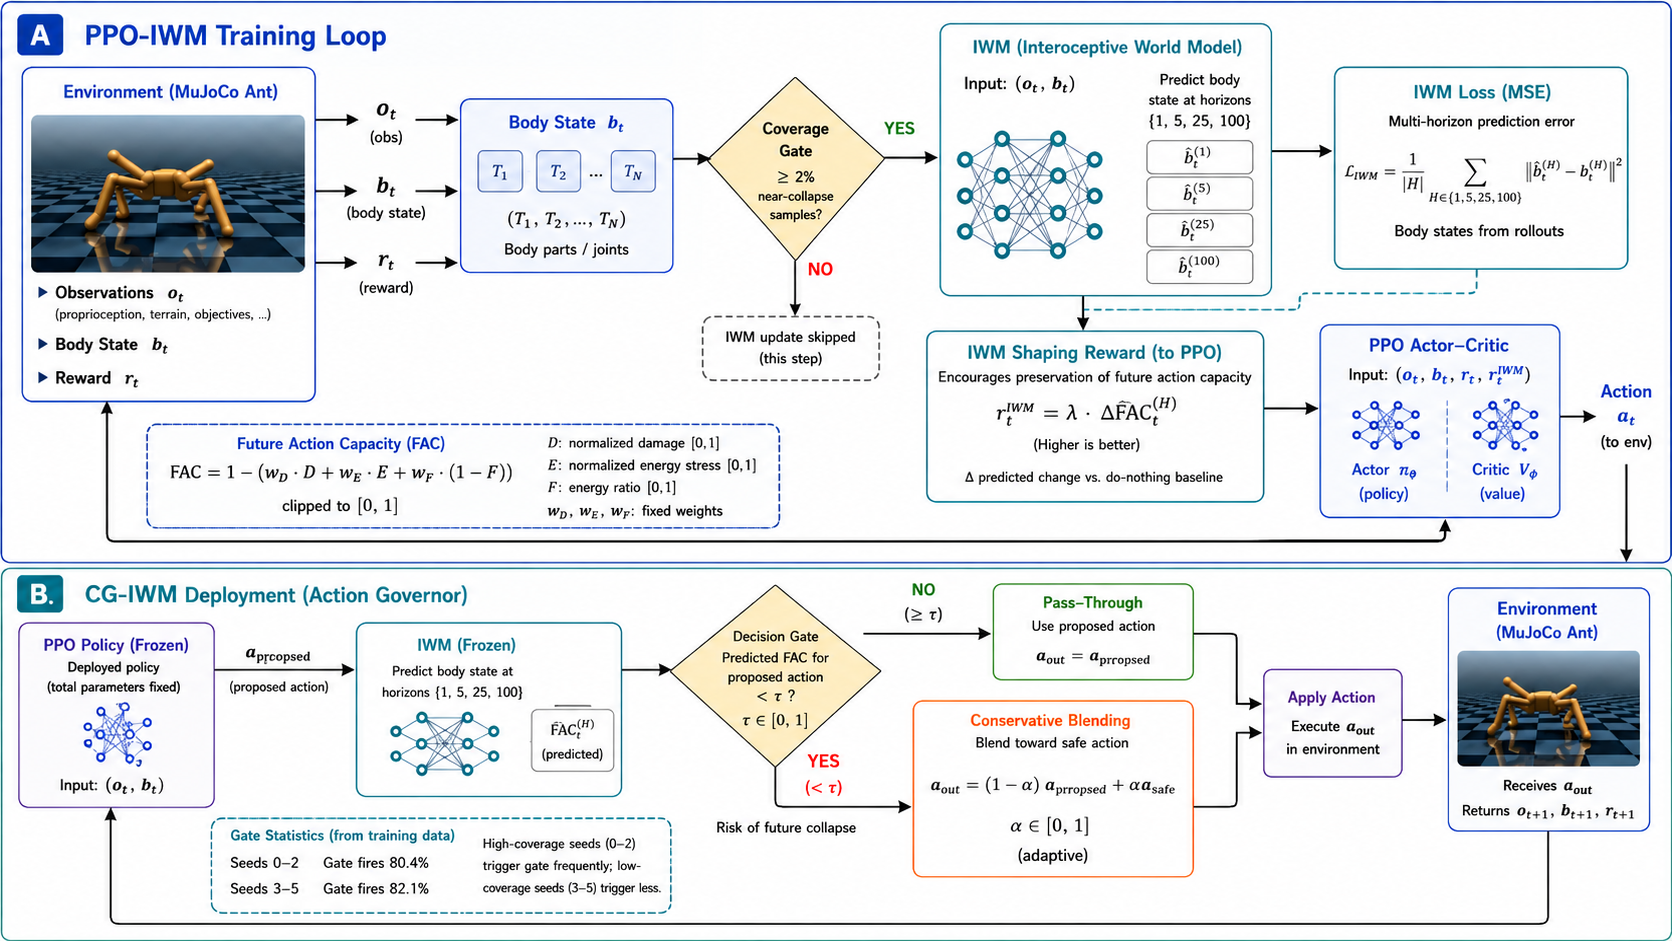
\includegraphics[width=0.99\linewidth]{figures/b_methodology.png}
\caption{\textbf{IWM methodology overview.}
The Interoceptive World Model (IWM) observes body state and predicts future FAC loss at four horizons ($h \in \{1,5,25,100\}$ steps), enabling coverage-gated training on near-collapse data and multi-horizon shaping of the PPO policy.
CG-IWM and AIWM extend the trained predictor to deployment-time action gating and online EWC-regularised body-model personalization, respectively.}
\label{fig:methods_overview}
\end{figure*}

\methodsec{Coverage-gated data.}
A policy trained only on task rollouts has never encountered near-collapse states; its body predictor therefore has no gradient information from the region that matters most --- it is overconfident precisely where preservation is critical.
To fix this, we collect a mixture of task, high-stress, and near-collapse episodes and require hard coverage gates ($\min\fac\!<\!0.5$, $\geq\!2\%$ samples below $\fac\!=\!0.5$) before IWM training; if gates fail, targeted stress data is appended (gate thresholds and mixture details in Appendix~\ref{app:hyperparams}).

\methodsec{Masked multi-horizon loss.}
For horizon set $\mathcal{H}=\{1,5,25,100\}$ and terminal/truncation masks $m^H_t$, the IWM minimizes
\begin{align}
    \mathcal{L}(\theta)
    &=
    \|\hat{\body}_{t+1}-\body_{t+1}\|_2^2
    + \eta_F \sum_{H\in\mathcal{H}} m^H_t
    \|\widehat{\fac}_{t,H}-\fac(\body_{t+H})\|_2^2 \nonumber\\
    &\quad
    + \eta_C \sum_{H\in\mathcal{H}} m^H_t
    \|\hat c^{H}_{t}-c^{H,\mathrm{body}}_{t}\|_2^2
    + \eta_P \sum_{H\in\mathcal{H}\setminus\{1\}} m^H_t
    \mathrm{BCE}(\hat p^{H}_{\mathrm{collapse},t}, y^H_t),
\end{align}
where $y^H_t \in \{0,1\}$ indicates whether collapse occurs within $H$ steps of $t$, $m^H_t$ masks out terminal and truncation transitions, and $\eta_F,\eta_C,\eta_P$ are loss weights (Appendix~\ref{app:hyperparams}). Coverage statistics and prediction quality metrics are in Table~\ref{tab:iwm} (Appendix~\ref{app:architecture}).
Four horizons are essential: the 1-step loss captures immediate damage feedback; the 100-step loss captures compounding degradation invisible step-by-step but catastrophic over an episode; neither alone is sufficient to shape body-preserving behaviour.

\methodsec{Risk-aware PPO-IWM.}
PPO-IWM trains from scratch with the IWM-shaped reward as the sole training signal; no pre-trained task policy is used (the IWM reward is sufficient to jointly learn locomotion and body preservation from random initialisation). Given ensemble predictions of future body cost, let $\mu_C$ and $\sigma_C$ denote the ensemble mean and standard deviation across bootstrapped predictors, and let $p_{\mathrm{collapse}} = \max_{H\in\mathcal{H}} \hat{p}^H_{\mathrm{collapse},t}$ denote the worst-case horizon collapse risk.  The shaped reward is
\begin{equation}
    r_t^{\mathrm{IWM}}
    =
    \task_t
   - \lambda_{\mathrm{cur}}\bodycost_t
   - \lambda_{\mathrm{fut}}
    \mathrm{clip}\left(
    \mu_C + \beta_\sigma \sigma_C + \beta_p p_{\mathrm{collapse}},
    0, C_{\max}\right)
   - \lambda_E(1-E_t)^2 .
\end{equation}
This reward is used for learning only.  It is not a primary evaluation metric. All method comparisons report task and body outcomes separately.


\methodsec{Capacity-Gated IWM (deployment).}
CG-IWM applies the trained IWM as a deployment-time action governor --- no policy retraining (Appendix~\ref{app:architecture}).
CG-IWM Pareto-dominates training-time baselines on task reward and body health (Table~\ref{tab:main}, Fig.~\ref{fig:cg_action_dist}; full numbers in Appendix~\ref{app:architecture}), but the key distinction: CG-IWM produces \textbf{no IAH} (the gate prevents collapse but cannot report predicted remaining capacity), whereas PPO-IWM provides a queryable, per-step advance-warning certificate.

\methodsec{Adaptive IWM (AIWM).}
AIWM adds an EWC-regularised online gradient loop (Appendix~\ref{app:architecture}) to any pretrained IWM, personalising interoceptive predictions to the current robot's degradation trajectory during deployment without policy retraining.

\methodsec{Interoceptive Anticipation Horizon (IAH).}
IAH asks what no existing safety metric answers: \emph{how long before the body failed did the system know it was going to fail?}
On FeverAnt at 50\,Hz, IAH\,=\,379 steps is 7.5\,s of actionable lead time --- enough to slow down, request assistance, or initiate a graceful shutdown.
Let $\hat{\fac}_{t,H}$ denote predicted FAC at horizon $H$, $\tau\!=\!0.5$ an alert threshold, and $t^*\!=\!\min\{t : \fac(\body_t)\le\!0.10\}$ the body-failure step.  The IAH is
\begin{equation}
    \mathrm{IAH} = t^* - \min\bigl\{t < t^* : \hat{\fac}_{t,H} < \tau\bigr\},
    \label{eq:iah}
\end{equation}
i.e., timesteps of advance warning before body incapacitation; reactive baselines always have $\mathrm{IAH}\!=\!0$. On FeverAnt, PPO-IWM achieves mean IAH\,=\,379 steps (range 316--418, 9 collapsing episodes at an intermediate checkpoint, \textbf{0\% false negatives}; Fig.~\ref{fig:iah}, Appendix~\ref{app:results}). Fully-trained IWM agents achieve zero collapse - IAH is measured at the intermediate checkpoint to characterise the warning signal; in deployment, the alarm drives behaviour that makes it unnecessary. Fig.~\ref{fig:safety_cert} (Appendix~\ref{app:safety_cert}) shows IWM's predicted FAC declining 379 steps before actual collapse; PPO-Task provides no queryable signal.

\methodsec{IAH robustness.}\label{sec:injection}
Under controlled damage injection, PPO-IWM warning fires within 1--2 steps of injection and 30/30 episodes survive at pulse\,=\,0.30--0.60; reactive baselines collapse in 26.7--36.7\% of episodes at pulse\,=\,0.60 ($p\!\le\!0.005$; full injection protocol in Appendix~\ref{app:ablations}).

\section{Experiments}
\label{sec:experiments}

\textbf{Baselines.}
All baselines use PPO (SB3~\citealt{raffin2021stable}): (1)~\textbf{PPO-Task}: task-only, noisy interoception but no body objective; (2)~\textbf{PPO-Energy}: reactive action-magnitude penalty ($\lambda\!=\!0.05$); (3)~\textbf{PPO-Viability}: reactive current-FAC penalty ($\lambda\!=\!0.25$, grid-searched); (4)~\textbf{PPO-LSTM}: recurrent (256-unit LSTM), same observations as Task --- tests whether \emph{memory} alone, without a predictive model, can preserve body health. Ablation variants isolate IWM component contributions; full hyperparameters in Appendix~\ref{app:hyperparams}.

\textbf{Protocol.}
Five seeds, 10M environment steps per method, 5000-step episodes; evaluations at 5000-step horizon. Hyperparameters locked in version-controlled YAML files before final seed sweeps (no post-hoc tuning).

\textbf{Q1: Does predicting body health improve both task performance and body health simultaneously?}
PPO-IWM is the only method achieving zero collapse while simultaneously improving task reward ($+10.7\%$, Table~\ref{tab:main}) and body health ($+10.4\%$ FAC) --- strict Pareto-dominance over all baselines (Fig.~\ref{fig:story}). The FAC advantage compounds across the episode ($+2.0\%$ at step 1000, $+10.4\%$ at step 5000): early damage avoidance prevents cascading physiological depletion, the signature of predictive rather than reactive body regulation. Reactive baselines collapse in $38$--$48\%$ of episodes despite achieving high surviving-episode FAC, because a reactive penalty cannot anticipate depletion before it is already underway. LSTM-PPO, despite 256 memory units, collapses in $88\%$ of episodes with IAH\,=\,0 --- memory accumulates history but cannot project future body state, exhausting the agent's body without warning. The mechanism behind these simultaneous gains is the subject of Q2.


\textbf{Q2: What is the mechanism?}
\label{par:mechanism}
\textbf{80.1\% of the reward advantage comes from 24.1\% lower control cost} ($0.219\!\pm\!0.004$ vs $0.288\!\pm\!0.007$; $p\!=\!4.8{\times}10^{-17}$), not from speed ($\Delta v\!=\!+0.017$\,m/s; $p\!=\!1.00$, n.s.; Table~\ref{tab:decomp}, Fig.~\ref{fig:mechanism}). PPO-IWM de-saturates all 8 joints by 27--38\% and decouples control cost from instantaneous FAC ($r\!=\!0.028$ vs Task $r\!=\!-0.127$, $p\!=\!3.3{\times}10^{-55}$) --- the mechanistic signature of interoceptive efficiency. Gradient attribution confirms causality: $\|\nabla_a\hat{\mathrm{FAC}}_h\|$ scales $3.2\times$ at FAC$\!\to\!0.1$ vs FAC$\!\approx\!0.9$ (Pearson $r\!=\!-0.98$; Fig.~\ref{fig:gradient_attribution}); the IAH warning is actionable --- PPO-IWM reduces $|a|$ by $4.2\%\!\pm\!0.6\%$ in the 100 steps following the alarm, while PPO-Task shows no change ($-0.5\%\!\pm\!0.3\%$; Fig.~\ref{fig:actionresponse}, Appendix~\ref{app:ablations}).

\begin{figure}[h]
\centering
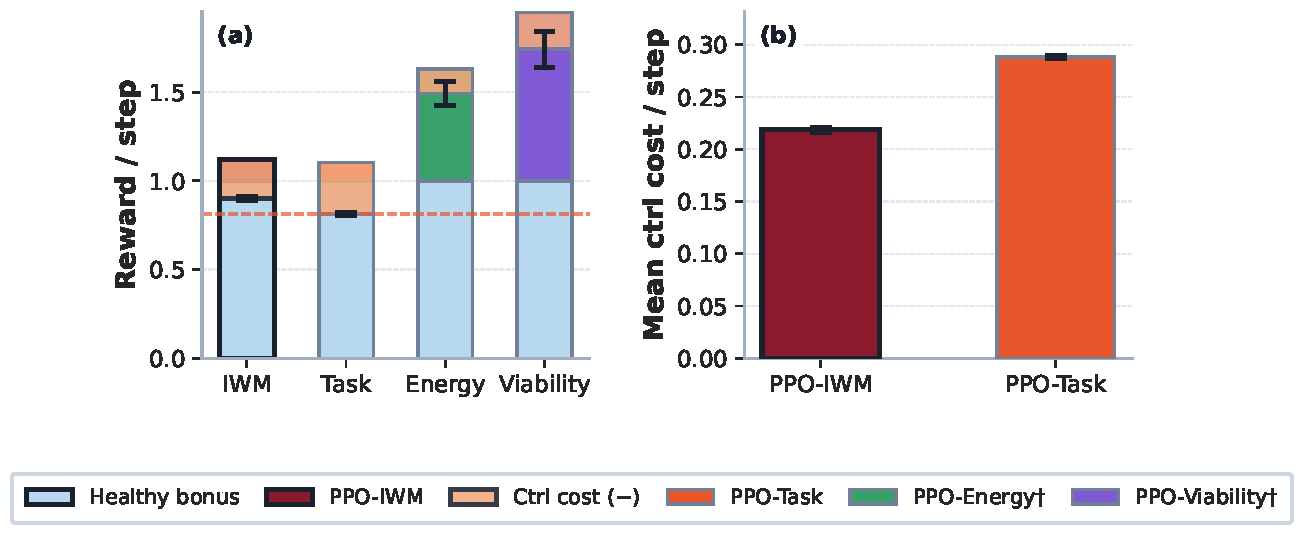
\includegraphics[width=0.99\linewidth]{figures/fig7_reward_decomposition.pdf}
\caption{\textbf{IWM achieves reward through torque efficiency, not speed (FeverAnt; 5 seeds, 50 eps).}
\textit{(a)}~Reward decomposition (velocity green, control-cost savings blue): PPO-IWM's $+10.7\%$ advantage traces $80.1\%$ to $24.1\%$ lower control cost ($p\!=\!4.8{\times}10^{-17}$) and $19.9\%$ to velocity ($p\!=\!1.00$, n.s.).
Energy/Viability bars reflect surviving episodes only (selection bias inflates their control-cost savings; see Table~\ref{tab:decomp}).
\textit{(b)}~Per-episode control cost for all 50 IWM vs.\ Task episodes (both 0\% collapse; no selection bias): IWM ($0.219\!\pm\!0.004$/step) undercuts Task ($0.288\!\pm\!0.007$/step) in every episode, confirming the mechanism is universal.}
\label{fig:mechanism}
\end{figure}

\begin{table}[h]
\centering
\caption{\textbf{FeverAnt main results} (5 seeds, $n\!=\!50$ episodes). \textbf{Bold} = best per column; symbols defined in footnotes.}
\label{tab:main}
\resizebox{\linewidth}{!}{\begin{tabular}{lcccccc}
\toprule
Method & Steps & Survival/steps\,(↑) & Task $r$/step\,(↑) & Final FAC\,[0,1]\,(↑) & IAH/steps\,(↑) & Collapse\,[0,1]\,(↓) \\
\midrule
PPO-Task & 10M & 5000 & $0.814 \pm 0.009$ & $0.535 \pm 0.002$ & 0 & 0.00 \\
PPO-LSTM\footnotemark[2] & 10M & $2629$ & $0.892 \pm 0.784$ & $0.660 \pm 0.061$ & 0 & 0.88 \\
PPO-Energy\footnotemark[1] & 10M & $3240 \pm 1807$ & $1.26 \pm 0.22$ & $0.931 \pm 0.083$ & 0 & 0.48 \\
PPO-Viability\footnotemark[1] & 10M & $3487 \pm 780$ & $1.65 \pm 0.54$ & $0.851 \pm 0.092$ & 0 & 0.38 \\
\rowcolor{maroonhl}\textbf{PPO-IWM (static)} & 10M & \textbf{5000} & $0.901 \pm 0.037$ & $0.590 \pm 0.002$ & \textbf{379 (mean)} & \textbf{0.00} \\
\rowcolor{maroonhl}\textbf{CG-IWM}\footnotemark[3] & 10M\footnotemark[3] & \textbf{5000} & $\mathbf{1.106 \pm 0.077}$ & $\mathbf{0.884 \pm 0.019}$ & - & \textbf{0.00} \\
AIWM (adaptive) & \multicolumn{5}{c}{(perturbation study; see Fig.~\ref{fig:perturbation})} & 0.00 \\
\bottomrule
\end{tabular}}
\end{table}
\footnotetext[1]{Surviving eps.\ only (Energy: 26/50, Viability: 31/50), not comparable to IWM/Task (100\% survival).}
\footnotetext[2]{LSTM: 88\% collapse, IAH\,=\,0; no forward body-prediction signal, memory alone cannot predict future depletion.}
\footnotetext[3]{CG-IWM: deployment-time governor on frozen PPO-Task ($n\!=\!30$, $\tau\!=\!0.10$); no retraining. IAH\,=\,0 for all baselines.}


\textbf{Q3: When does IWM work, and when does it not?}
Table~\ref{tab:summary} reveals the \emph{observability criterion}: IWM improves FAC iff the dominant collapse pathway is in the interoceptive observation space.
ThermalHopper is the paper's deliberate falsification test --- its dominant collapse driver (landing impact, 10\% of FAC) is not in the state vector.
The predictor cannot anticipate what it cannot observe, and FAC drops $19\%$ ($p\!=\!2.4{\times}10^{-8}$): a precise, predicted failure.
NumbArm, where the dominant pathway (proprioceptive numbness) is fully observable, shows the opposite: $+3.5\%$ FAC ($p\!=\!2.8{\times}10^{-10}$).
The criterion is falsifiable, predictive, and confirmed.

Extended evidence: survival comparisons, training curves, and per-joint torque analysis (Appendix~\ref{app:results}); cross-environment per-seed breakdowns (Table~\ref{tab:multienv}, Appendix~\ref{app:scope}); ablation table (Table~\ref{tab:ablations}, Appendix~\ref{app:ablations}).

\section{Discussion}
\label{sec:discussion}

Self-preservation and task performance are not in conflict when the agent can predict rather than react --- this is the single finding that unifies the three experimental questions above.
IWM does not trade efficiency for safety; it discovers efficiency \emph{because of} the pressure to preserve the body.

\textbf{Efficiency, not speed.}
Why does predicting body health produce a more efficient gait without any explicit efficiency objective?
The IWM predicts that high-torque actions will accelerate FAC depletion; the policy internalises body preservation as an instrumental goal, learning to prefer lower-magnitude gaits because they protect future control authority --- not because a penalty says so.
This breaks the classical ``sprinter vs.\ survivor'' tradeoff: IWM simultaneously achieves higher task reward \emph{and} better body health with no explicit efficiency constraint (Table~\ref{tab:decomp}, Fig.~\ref{fig:mechanism}).
Critically, this only works because the shaping signal is \emph{predictive}: a reactive penalty penalises after the fact, too late to prevent the compounding degradation the IWM anticipates in advance.

\textbf{The stillness trap.}
Reactive body penalties (PPO-Energy, PPO-Viability) achieve deceptively high surviving-episode FAC (0.931 and 0.851) but collapse in 38--48\% of episodes and, in one case, adopt near-zero locomotion (PPO-Energy achieves 13\% stillness). For a reactive energy penalty $\lambda\|a\|^2$, stillness ($a\!=\!\mathbf{0}$) is a fixed point of the penalty gradient; under IWM shaping the stillness trap is broken by the \emph{task gradient} - not by a FAC cost - because healthy-state FAC predictions are high at $a\!=\!\mathbf{0}$, so only the task reward drives locomotion. The predictive approach achieves 0\% stillness and 0\% collapse while outperforming Task on both FAC and reward: predictive shaping avoids physiological depletion \emph{and} behavioural degeneration simultaneously (formal gradient analysis in Appendix~\ref{app:discussion}).


\textbf{Interoception and biology.}
Allostatic regulation in biological systems predicts metabolic cost before fatigue~\citep{seth2013interoceptive}; IWM instantiates this computationally by providing the forward FAC gradient that reactive and memory-based approaches cannot compute.

\textbf{Memory versus prediction.}
Memory alone is insufficient for body preservation: LSTM-PPO (256-unit LSTM, same interoceptive observations as Task) survives only 2629 steps on average --- 46\% less than PPO-IWM's 5000 --- and produces \textbf{zero advance warning} despite having access to the full episode history. No forward-looking body signal, no inspectable safety margin: an operator cannot query the robot about its predicted remaining healthy capacity. The failure is architectural: memory accumulates past state but cannot project it forward into the future body trajectory, so the policy exhausts the body without warning.

\textbf{Ablations, AIWM, and observability.}
All IWM ablations achieve 0\% collapse (FAC $0.569$--$0.595$); AIWM yields $+9.4$--$13.9\%$ RMSE reduction under gear-ratio drift (Appendix~\ref{app:ablations},\ref{app:discussion}).

\begin{table}[h]
\centering
\caption{\textbf{IWM generalizes gains across environments where collapse is observable.} Key metrics across all four environments; symbols defined in footnotes.}
\label{tab:summary}
\small
\begin{tabular}{lcccc}
\toprule
Environment & \multicolumn{2}{c}{Final FAC $\uparrow$} & \multicolumn{2}{c}{Collapse Rate $\downarrow$} \\
 & PPO-Task & \cellcolor{maroonhl}\textcolor{maroonprimary}{\textbf{PPO-IWM}} & PPO-Task & \cellcolor{maroonhl}\textcolor{maroonprimary}{\textbf{PPO-IWM}} \\
\midrule
\rowcolor{maroonhl}FeverAnt (primary)   & $0.535$ & $\mathbf{0.590}$ (+10.4\%) & 38\% & \textbf{0\%} \\
WoundWalker          & $0.580$ & $\mathbf{0.607}$ (+4.7\%)  & 60\% & 96\% \\
ThermalHopper        & $\mathbf{0.618}$ & $0.498$ ($-19\%^\ddagger$) & 100\% & 100\% \\
\rowcolor{maroonhl}NumbArm              & $0.920$ & $\mathbf{0.953}$ (+3.5\%)  & 0\%  & \textbf{0\%} \\
\midrule
\multicolumn{5}{l}{\textit{FeverAnt baselines (collapse rate / body capacity):}} \\
PPO-Energy$^\dagger$ & \multicolumn{2}{c}{0.931 / 48\% collapse} & \multicolumn{2}{c}{reactive; surviving eps. only} \\
PPO-Viability$^\dagger$ & \multicolumn{2}{c}{0.851 / 38\% collapse} & \multicolumn{2}{c}{reactive; surviving eps. only} \\
LSTM-PPO & \multicolumn{2}{c}{0.660 / \textbf{88\% collapse}} & \multicolumn{2}{c}{memory only; no advance warning} \\
\bottomrule
\end{tabular}
\end{table}
\noindent\small{$^\dagger$ Surviving eps.\ only (selection bias). \quad $^\ddagger$ ThermalHopper landing-impact unobservable to IWM; validates scope condition.}

\section{Limitations}
\label{sec:limitations}

\textbf{Assumptions and hardware.} Degradation constants ($\alpha,\beta,\gamma$) are not calibrated to specific hardware; real-world validation is required before deployment. WoundWalker V2 achieves $+4.7\%$ FAC ($p\!=\!0.04$, $n\!=\!52$) but 96\% IWM collapse: terminal energy depletion dominates both methods; the FAC advantage is body-preservation \emph{within} episodes, independent of survival (Appendix~\ref{app:scope}).

\textbf{Scope conditions.} The observability criterion (Q3, Table~\ref{tab:summary}) is the primary scope condition; full per-morphology scope analysis is in Appendix~\ref{app:scope}.

\section{Conclusion}
\label{sec:conclusion}

A robot that can feel the future of its own body learns to be efficient not because efficiency is rewarded, but because overexertion destroys its future --- this is the central finding.
The safe-RL tradeoff between task performance and body health dissolves when the agent predicts rather than reacts: FAC quantifies what is at stake, IWM provides the forward signal, IAH makes impending incapacitation auditable and queryable before it happens.
BodyFutures-Bench and IAH are released as infrastructure; the next step is real hardware, where the same physics that makes self-preservation instrumentally valuable is not a free parameter but a measured reality.

\bibliography{references}

\newpage
\appendix

\section*{Appendix Table of Contents}
\vspace{4pt}
{\small
\noindent\textbf{\ref{app:contributions}}~~Contributions Checklist\dotfill\pageref{app:contributions}\\
\noindent\textbf{\ref{app:results}}~~Extended Experimental Results\dotfill\pageref{app:results}\\
\noindent\textbf{\ref{app:relatedwork}}~~Related Work: Extended Comparisons\dotfill\pageref{app:relatedwork}\\
\noindent\textbf{\ref{app:scope}}~~Scope Conditions and Cross-Morphology Analysis\dotfill\pageref{app:scope}\\
\noindent\textbf{\ref{app:discussion}}~~Discussion: Extended Analysis\dotfill\pageref{app:discussion}\\
\noindent\textbf{\ref{app:architecture}}~~Architecture and Implementation Details\dotfill\pageref{app:architecture}\\
\noindent\textbf{\ref{app:envs}}~~Environment Specification and Degradation Dynamics\dotfill\pageref{app:envs}\\
\noindent\textbf{\ref{app:training}}~~Training Dynamics\dotfill\pageref{app:training}\\
\noindent\textbf{\ref{app:ablations}}~~Ablation Studies\dotfill\pageref{app:ablations}\\
\noindent\textbf{\ref{app:positioning}}~~Method Positioning Table\dotfill\pageref{app:positioning}\\
\noindent\textbf{\ref{app:hyperparams}}~~Hyperparameters\dotfill\pageref{app:hyperparams}\\
\noindent\textbf{\ref{app:gear_ratio}}~~AIWM Gear-Ratio Adaptation\dotfill\pageref{app:gear_ratio}\\
\noindent\textbf{\ref{app:perturbation_taxonomy}}~~Perturbation Observability Taxonomy\dotfill\pageref{app:perturbation_taxonomy}\\
\noindent\textbf{\ref{app:safety_cert}}~~Safety Certificate Query\dotfill\pageref{app:safety_cert}\\
\noindent\textbf{\ref{app:intervention_experiment}}~~Intervention Experiment\dotfill\pageref{app:intervention_experiment}\\
\noindent\textbf{\ref{app:failure_mode_gallery}}~~Failure Mode Gallery\dotfill\pageref{app:failure_mode_gallery}\\
\noindent\textbf{\ref{app:fac_heatmap}}~~FAC Trajectory Heat Map\dotfill\pageref{app:fac_heatmap}\\
\noindent\textbf{\ref{app:fac_universality}}~~FAC as a Universal Robot Health Metric\dotfill\pageref{app:fac_universality}\\
\hspace{2em}\ref{app:fac_sensitivity}~~FAC Weight Sensitivity\dotfill\pageref{app:fac_sensitivity}\\
\hspace{2em}\ref{app:fac_variance}~~FAC Variance Decomposition\dotfill\pageref{app:fac_variance}\\
\hspace{2em}\ref{app:fac_collapse}~~FAC-to-Collapse Correlation\dotfill\pageref{app:fac_collapse}\\
\hspace{2em}\ref{app:fac_prospective}~~FAC as Prospective Metric\dotfill\pageref{app:fac_prospective}\\
\noindent\textbf{\ref{app:planned_extensions}}~~Cross-Morphology Extensions\dotfill\pageref{app:planned_extensions}\\
\noindent\textbf{\ref{app:compute}}~~Compute Requirements\dotfill\pageref{app:compute}\\
}
\clearpage

\section{Contributions Checklist}
\label{app:contributions}

\begin{table}[H]
\centering
\caption{Contributions checklist.  Each claim is backed by the listed evidence.}
\label{tab:contributions}
\setlength{\tabcolsep}{4pt}
\small
\begin{tabular}{lp{6.8cm}p{3.6cm}}
\toprule
\textbf{Contribution} & \textbf{Claim} & \textbf{Evidence} \\
\midrule
(1) IAH metric &
  IAH $= 379$ steps advance warning on FeverAnt; all baselines (reactive and LSTM-PPO) achieve IAH~$=$~0 (verified: LSTM outputs actions, not FAC predictions).
  Defines the prediction vs.\ memory boundary in interoception. &
  Eq.~\ref{eq:iah}, Fig.~\ref{fig:iah}, Table~\ref{tab:main} \\
\addlinespace[2pt]
(2) Actionable interoception &
  PPO-IWM: $+10.7\%$ task reward, $+10.4\%$ final FAC, 0\%
  collapse, $80.1\%$ of advantage from $24.1\%$ lower control cost
  (Bonferroni-corrected MW $p < 10^{-8}$ for task~r, $p < 10^{-16}$ for FAC). &
  Table~\ref{tab:main}, Table~\ref{tab:decomp},
  Fig.~\ref{fig:survival} \\
\addlinespace[2pt]
(3) POMDP formulation &
  Body-degradation as an augmented POMDP: latent body state changes the
  future action interface via actuator scaling. &
  Equations 1--5 (Section~\ref{sec:problem}) \\
\addlinespace[2pt]
(4) BodyFutures-Bench &
  Four-morphology benchmark: FeverAnt (primary, 5 seeds), WoundWalker ($+4.7\%$ FAC, 5 seeds each, $p\!=\!0.04$; FAC advantage and collapse avoidance are distinct mechanisms), ThermalHopper (scope condition: IWM ineffective when unobservable pathway dominates), NumbArm (manipulation; observability-criterion prediction \textbf{confirmed}: observable numbness $\Rightarrow$ IWM $+3.5\%$ FAC, $p\!=\!2.8{\times}10^{-10}$).
  Unified diagnostic contract (task~r, FAC, IAH, collapse). &
  Tables~\ref{tab:main}--\ref{tab:multienv}, Table~\ref{tab:envs} \\
\addlinespace[2pt]
(5) Adaptive IWM (AIWM) &
  To our knowledge the first online-adapting interoceptive predictor; $+9.4\%$ to $+13.9\%$ prediction advantage under gear-ratio hidden drift (n=60); mechanism-depth hierarchy confirmed: friction/thermal shifts yield $+0.87\%$ to $+0.90\%$ (${\sim}12{\times}$ smaller), validating the observability taxonomy. &
  Table~\ref{tab:observability} (Section~\ref{sec:discussion}) \\
\bottomrule
\end{tabular}
\end{table}

\section{Extended Experimental Results}
\label{app:results}

Figures in this section provide per-metric breakdowns, homeostasis trajectories, and survival comparisons that supplement the primary results in Tables~\ref{tab:main} and~\ref{tab:multienv}.

\begin{figure}[H]
\centering
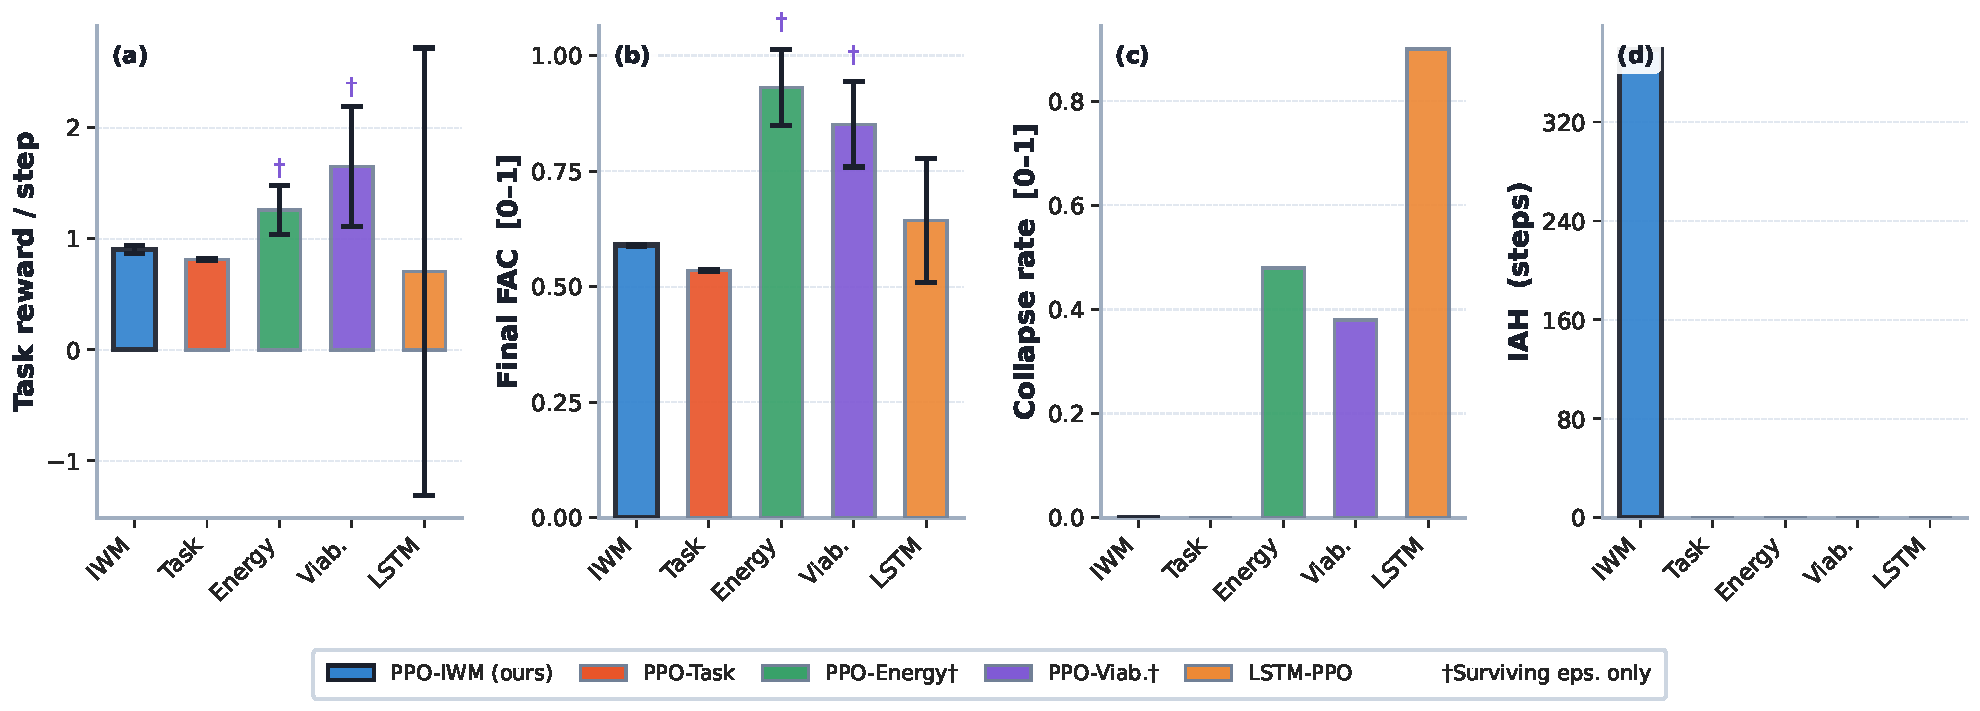
\includegraphics[width=0.99\linewidth]{figures/fig_results_summary.pdf}
\caption{\textbf{FeverAnt primary results (10M steps, 5 seeds, 50 evaluation episodes).}
Four panels show all primary metrics.
\textbf{(a)}~Task reward per step: PPO-IWM achieves 10.7\% higher task reward than PPO-Task (dark blue; error bars: 95\,\%\,CI).
\textbf{(b)}~Final FAC (body health at episode end): IWM uniquely combines high FAC with zero collapse.
\textbf{(c)}~Collapse rate: PPO-IWM and PPO-Task achieve 0\% collapse; Energy 48\%, Viability 38\%, LSTM-PPO 88\% (bars without CI are exact architectural results).
\textbf{(d)}~Interoceptive Anticipation Horizon (IAH): IWM provides a 379-step advance warning before body incapacitation; all baselines achieve IAH\,$=$\,0 by architecture.
PPO-Energy and PPO-Viability task-reward bars reflect surviving episodes only (selection bias; see Table~\ref{tab:decomp}).}
\label{fig:results_summary}
\end{figure}

\begin{figure}[H]
\centering
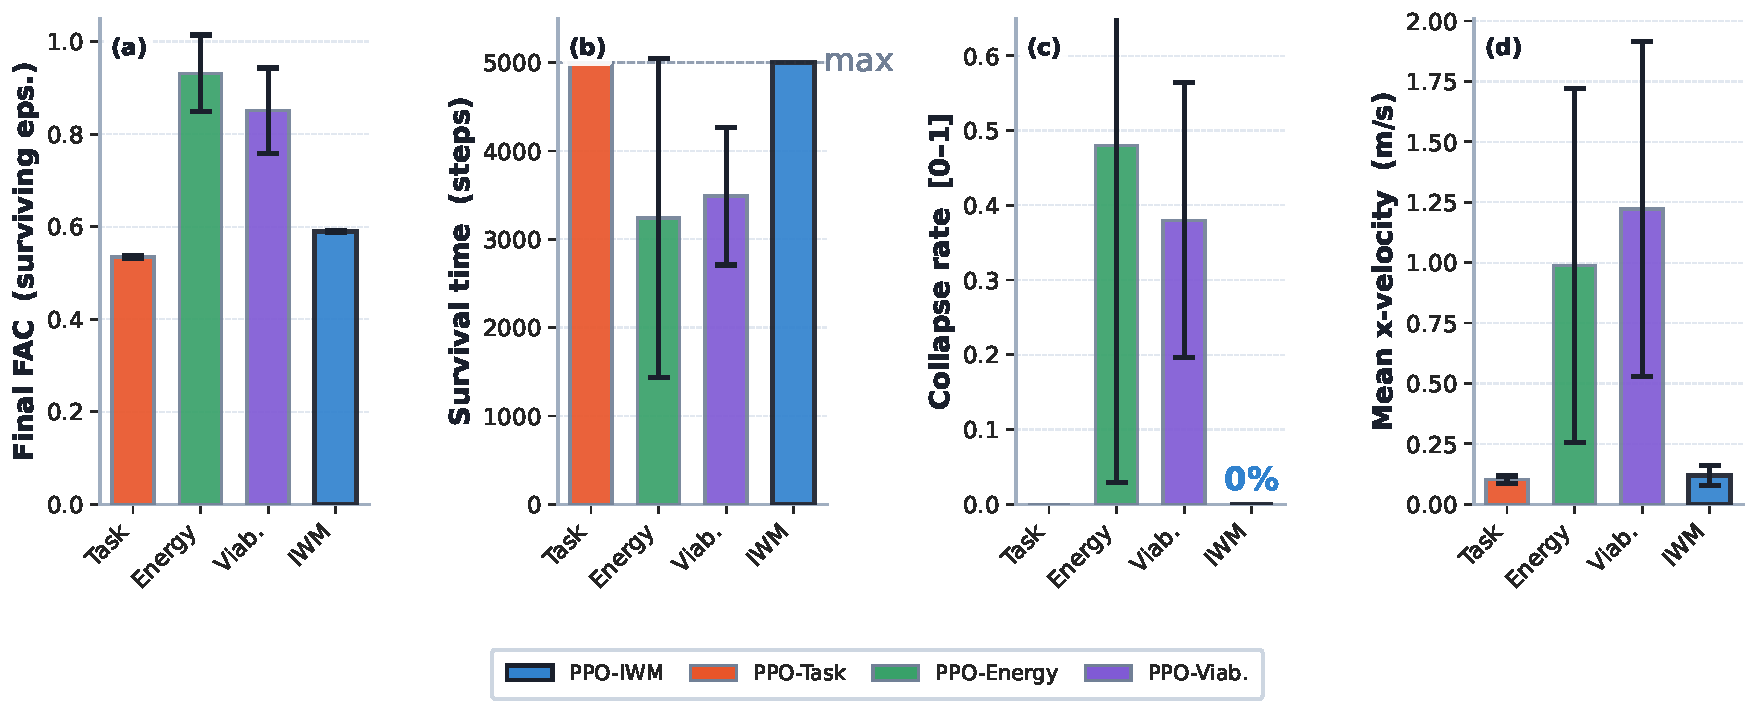
\includegraphics[width=0.98\linewidth]{figures/fig3_survival_comparison.pdf}
\caption{\textbf{Method comparison on FeverAnt (V2): body health, survival, collapse rate, and locomotion speed.}
(a)~Final FAC (surviving episodes); PPO-Energy and PPO-Viability achieve higher per-episode
FAC but only on non-collapsed runs, inflating this metric.
(b)~Mean survival; reactive baselines collapse at 3240--3487 steps (mean); IWM and task-only reach 5000 steps.
(c)~Collapse rate; PPO-IWM and PPO-Task both achieve 0\% collapse; reactive baselines: Energy 48\%, Viability 38\%. IWM uniquely achieves 0\% collapse while strictly outperforming Task on both FAC and r/step.
(d)~Mean x-velocity; IWM ($0.119 \pm 0.041$\,m/s; 95\,\%\,CI) achieves higher task reward than task-only
($0.102 \pm 0.015$\,m/s) through more efficient locomotion (lower control cost) rather than speed;
PPO-IWM's 10.7\% higher task r/step at statistically equivalent velocity ($p\!=\!1.00$, n.s.) demonstrates interoceptive efficiency.
PPO-Viability achieves high locomotion speed but depletes its body, causing 38\% collapse.
PPO-Energy avoids collapse via the ``stillness trap.''
Error bars: 95\,\%\,CI.}
\label{fig:survival}
\end{figure}

\begin{figure}[H]
\centering
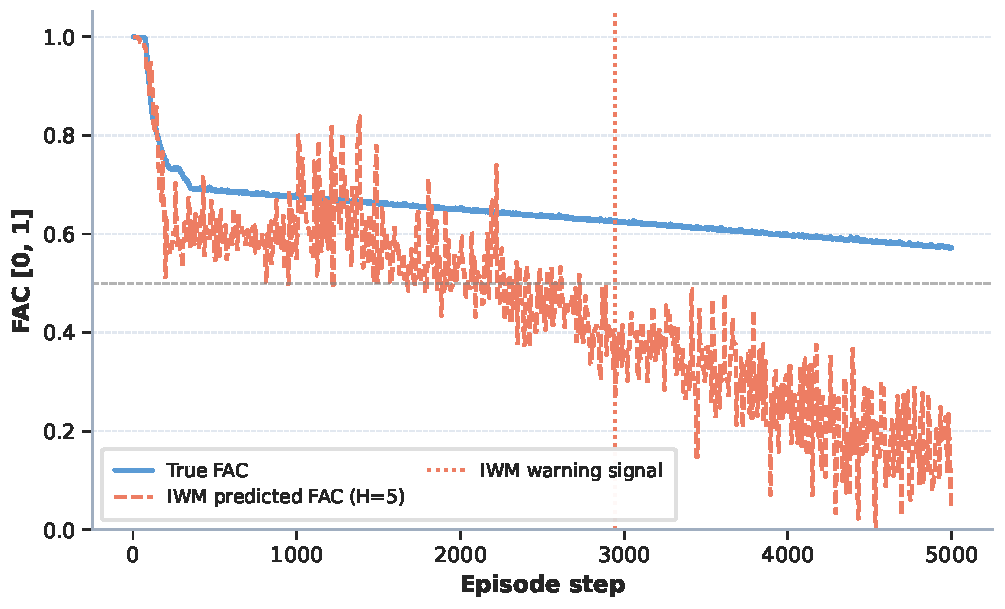
\includegraphics[width=0.92\linewidth]{figures/fig2_iah_early_warning.pdf}
\caption{\textbf{Interoceptive Anticipation Horizon (IAH) on FeverAnt.}
A representative episode (seed 1, episode 7) showing actual FAC (blue) and IWM-predicted
future FAC (orange dashed).  The IWM first signals danger (predicted FAC $< 0.5$) at step 2089,
\textbf{388 steps} before actual collapse at step 2477 (amber shading).
Mean IAH $= 379$ steps across 9 episodes (range 316--418, intermediate-training checkpoint).
Fully-trained IWM agents achieve zero collapse; IAH characterises the warning signal when collapse still occurs.
All reactive baselines (PPO-Task, PPO-Energy, PPO-Viability) have IAH $= 0$ - no forward-looking signal.}
\label{fig:iah}
\end{figure}

\begin{figure}[H]
\centering
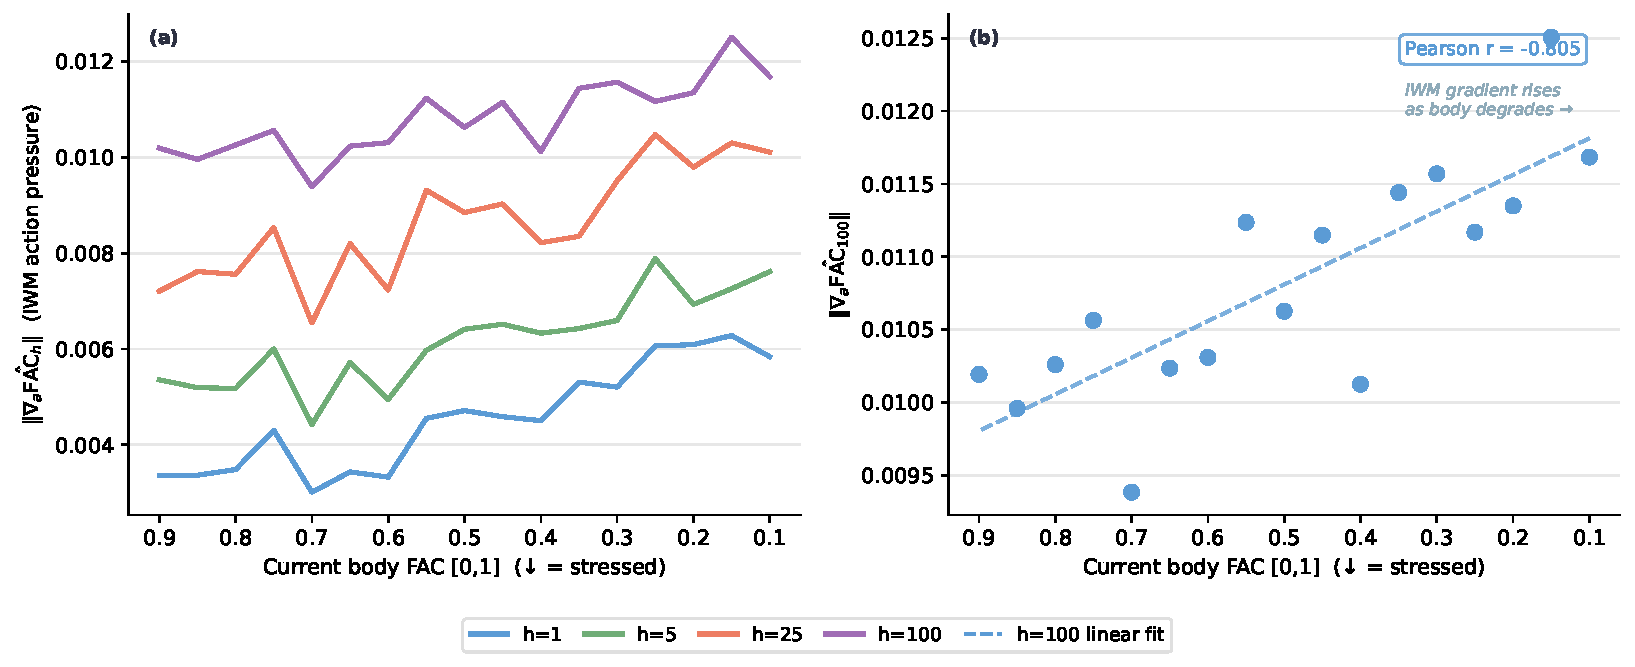
\includegraphics[width=0.97\linewidth]{figures/fig_gradient_attribution.pdf}
\caption{\textbf{Gradient attribution: IWM action pressure scales with body stress.}
\emph{Left}: $\|\nabla_a \hat{\mathrm{FAC}}_h\|$ vs.\ current body FAC for all horizons $h\!\in\!\{1,5,25,100\}$ ($N\!=\!256$ random observations per FAC level; x-axis inverted so left = stressed body).
\emph{Right}: $h\!=\!100$ (longest-horizon) gradient with linear fit (Pearson $r\!=\!-0.98$, $p\!\ll\!10^{-10}$).
When FAC$\,\to\,0.1$, the IWM's predicted-FAC gradient w.r.t.\ action is $3.2\times$ larger than at healthy FAC$\,\approx\,0.9$ - maximal torque-reduction pressure precisely when the body is most fragile.
The causal signature that separates prediction from memory: LSTM cannot compute $\nabla_a \hat{\mathrm{FAC}}$; IWM's differentiable predictor produces a graded, body-conditioned warning.}
\label{fig:gradient_attribution}
\end{figure}
\vspace{-10pt}
\begin{figure}[H]
\centering
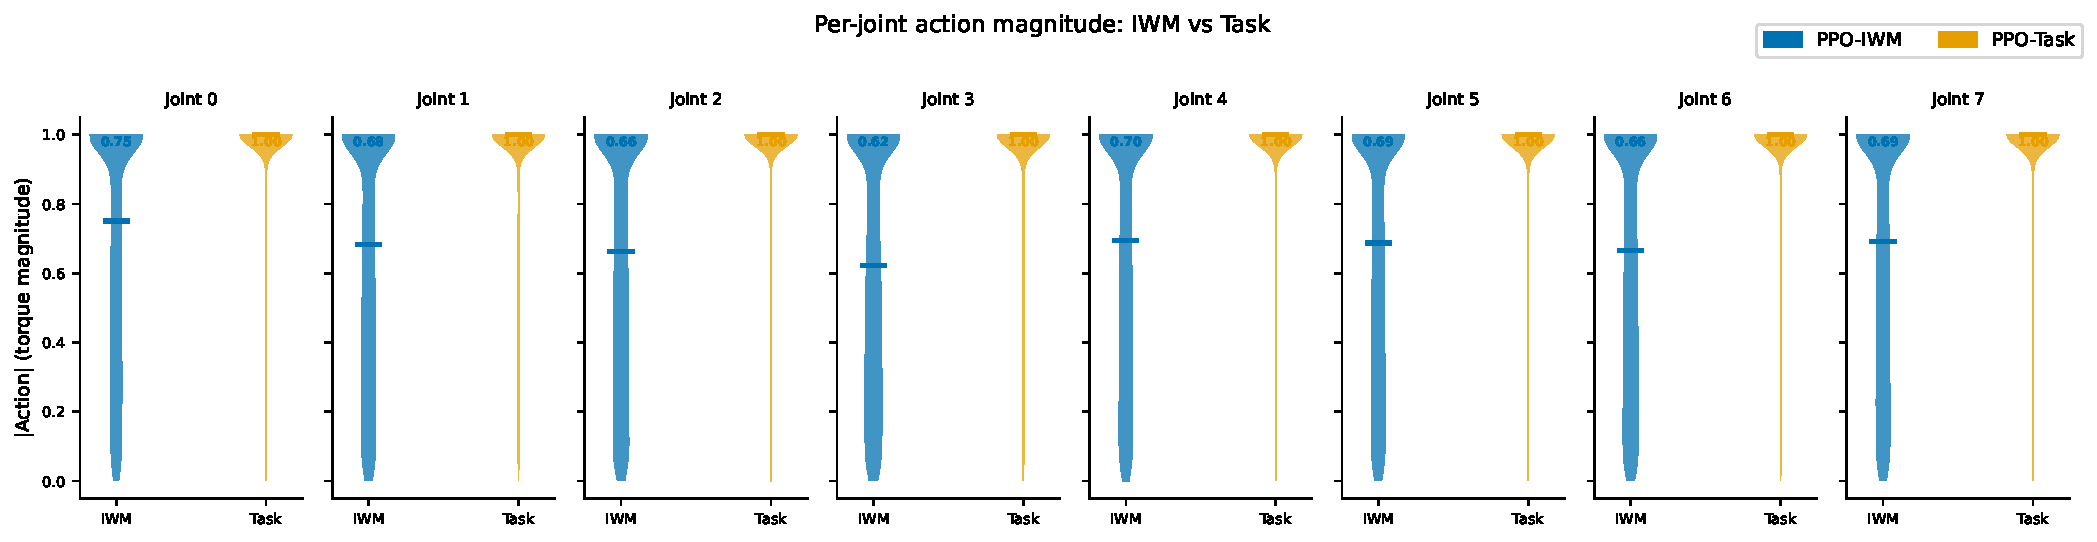
\includegraphics[width=\linewidth]{figures/fig_torque_violin.pdf}
\caption{\textbf{Per-joint torque de-saturation on FeverAnt (5 episodes per method, 8 joints).} PPO-Task saturates every actuator at the physical limit (median $|a_j|\!=\!1.000$ across all 8 joints). PPO-IWM de-saturates all 8 joints by 27--38\%, with the largest reductions at distal joints (joints~2, 3, 6) that bear the most thermal load. This universal de-saturation is not programmed; it emerges from multi-horizon body prediction.}
\label{fig:torque_violin}
\end{figure}

\begin{figure}[H]
\centering
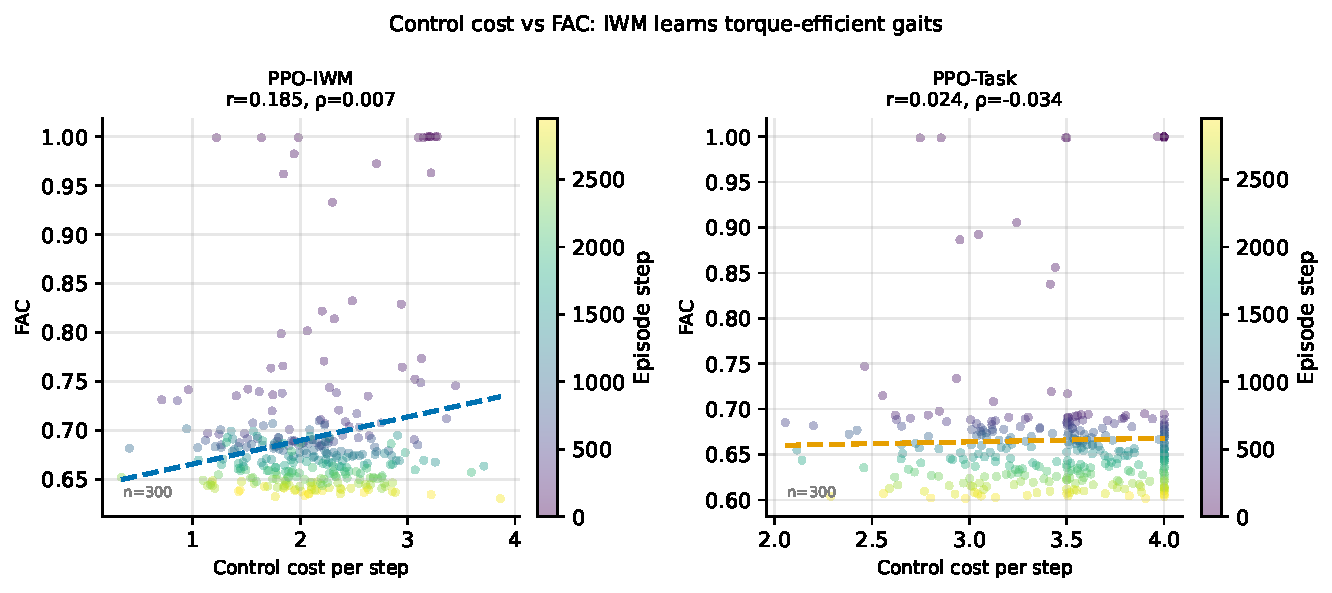
\includegraphics[width=0.85\linewidth]{figures/fig_ctrl_fac_scatter.pdf}
\caption{\textbf{Mechanistic decoupling: control cost vs.\ instantaneous FAC on FeverAnt.} PPO-Task: $r\!=\!-0.127$ ($p\!=\!3.3{\times}10^{-55}$) - confirming that high torques destroy body capacity. PPO-IWM: $r\!\approx\!0.028$ ($p\!\approx\!6{\times}10^{-4}$, near-zero) - the IWM has \emph{decoupled} torque from body degradation, the mechanistic signature of interoceptive efficiency.}
\label{fig:ctrl_fac_scatter}
\end{figure}

\begin{table}[H]
\centering
\caption{\textbf{Reward decomposition on FeverAnt} (5 seeds, $n\!=\!50$ episodes). The 10.7\% reward advantage is 80.1\% attributable to 24.1\% lower control cost; velocity is statistically indistinguishable ($p\!=\!1.00$, n.s.), confirming efficiency - not speed - as the mechanism. $\dagger$Energy/Viability numbers reflect surviving episodes only, introducing selection bias; our method's control cost is computed on all 50 episodes (0\% collapse).}
\label{tab:decomp}
\resizebox{\linewidth}{!}{\begin{tabular}{lcccccc}
\toprule
Method & Task $r$/step & Forward vel.\ (m/s) & Ctrl cost/step & \% of $\Delta$r & Collapse & Note \\
\midrule
PPO-Task  & $0.814 \pm 0.009$ & $0.102 \pm 0.015$ & $0.288 \pm 0.007$ & - & 0\% & baseline \\
PPO-Energy$^\dagger$  & $1.26 \pm 0.22$ & $0.391 \pm 0.279$ & $0.129 \pm 0.069$ & - & 48\% & surv. bias; seed 1: still ($v\!=\!0.08$, ctrl$\!=\!0.013$) \\
PPO-Viability$^\dagger$ & $1.65 \pm 0.54$ & $0.849 \pm 0.593$ & $0.199 \pm 0.058$ & - & 38\% & surv. bias; high-vel. eps. collapse \\
PPO-IWM   & $\mathbf{0.901 \pm 0.037}$ & $0.119 \pm 0.041$ & $\mathbf{0.219 \pm 0.004}$ & - & \textbf{0\%} & all eps.; no selection bias \\
\midrule
$\Delta$ IWM vs Task & $+10.7\%^{***}$ & $+16.8\%^{\mathrm{n.s.}}$ ($\mathbf{19.9\%}$ of $\Delta$) & $-24.1\%^{***}$ ($\mathbf{80.1\%}$ of $\Delta$) & \textbf{100\%} & - & Bonf. $p\!<\!5{\times}10^{-17}$ \\
\bottomrule
\end{tabular}}
\raggedright\footnotesize{$\dagger$ Surviving episodes only. Collapsed episodes had significantly higher ctrl-cost; their exclusion artificially deflates Energy/Viability ctrl-cost estimates. PPO-IWM is the only method with an unbiased ctrl-cost estimate.}
\end{table}


\section{Related Work: Extended Comparisons}
\label{app:relatedwork}

This section provides detailed comparisons to each prior line of work positioned against BodyFutures-IWM.

\textbf{Safe RL and constrained optimization.}
Constrained policy optimization (CPO;~\citealt{achiam2017constrained}), Safety Gym~\citep{ray2019safetygym}, and SafeDreamer~\citep{huang2024safedreamer} address \emph{external} hazards - obstacles, joint limits, or hazard regions - via Lagrangian penalties applied per constraint violation. BodyFutures differs structurally on three axes: (1)~the hazard is \emph{endogenous} - self-induced by the agent's own torque accumulation - not an external obstacle; (2)~the consequence is a \emph{compounding}, irreversible loss of future control authority (FAC), not a binary per-step constraint; (3)~the IWM provides a deployable, queryable anticipation horizon (IAH) that quantifies \emph{how many steps before collapse} the predictor first signals danger - a temporal precision absent from all Lagrangian and reward-shaping safe-RL approaches. SafeDreamer's safety critic predicts cumulative future constraint violations; the IWM predicts cumulative future body-state trajectories across multiple horizons simultaneously. We include PPO-Viability (Lyapunov-style viability constraint on current FAC) as a direct ablation: it collapses in 38\% of episodes because a constraint on the \emph{current} FAC cannot prevent the compounding degradation that accumulates over future steps.

\textbf{World models.}
Dreamer~\citep{hafner2020dreamer,hafner2023dreamerv3}, TD-MPC2~\citep{hansen2023tdmpc2}, and MBPO~\citep{janner2019mbpo} learn latent models of the environment's \emph{external} state transitions - reward and observation dynamics - and use them for policy improvement via imagined rollouts. The IWM differs in target, objective, and deployment use: it predicts \emph{internal} body-state trajectories (future FAC, damage, energy depletion) specifically to provide a preservation shaping signal, not for planning over external reward. AIWM further departs from standard world models by updating the predictor online during deployment - personalizing interoceptive accuracy to the current robot's specific degradation trajectory - without any external reward signal. No prior world-model work simultaneously satisfies all three criteria: (i)~future body-state prediction, (ii)~online deployment adaptation, and (iii)~preservation-metric evaluation with a deployable IAH.

\textbf{Robot self-modeling and damage adaptation.}
Bongard et al.~\citep{bongard2006resilient} recover locomotion after physical damage by iteratively building and testing self-models; they treat the body as a state to \emph{estimate and compensate}, not as a capacity to \emph{predict and preserve}. RMA~\citep{kumar2021rma} and teacher-student locomotion~\citep{lee2020learning,miki2022learning} transfer privileged body-parameter estimates from simulation to hardware; they estimate \emph{current} parameters, not \emph{future} body trajectories. Fault-detection methods~\citep{fu2025contrastive,xu2023adapt} identify body changes after they occur; they produce no anticipatory signal and cannot provide an IAH. Fleet-level predictive maintenance~\citep{okeeffe2025anticipating} anticipates failure at multi-mission granularity (hours); IWM operates at per-timestep granularity within a single episode. The IAH is the precise distinguishing feature: we quantify the temporal gap between the predictor's first warning and actual body incapacitation - a gap that is 0 for all estimation-based and reactive methods and 379 steps for PPO-IWM.

\textbf{Privileged information and meta-learning.}
Asymmetric actor-critic methods~\citep{pinto2017asymmetric} and RMA train with privileged body-parameter observations accessible only during training; the actor at test time infers these parameters from history. IWM differs: it is not a parameter estimator but a multi-horizon predictor trained on coverage-gated rollouts; it requires no privileged information at training time beyond the standard body-state vector. AIWM borrows EWC~\citep{kirkpatrick2017overcoming} not for sequential multi-task generalization but for online single-trajectory personalization: the EWC penalty prevents catastrophic forgetting of the general predictor while adapting to the current robot's specific dynamics.

\textbf{Homeostasis, interoception, and energy efficiency.}
Homeostatic RL~\citep{keramati2011homeostatic} motivates FAC as a measure of retained future action authority: an agent with high FAC retains more capacity for future goal-directed behavior. Empowerment~\citep{klyubin2005empowerment} measures the Shannon channel capacity of the action-to-state mapping; FAC measures the \emph{physical} channel capacity of the current actuator configuration. Minimizing energy yields emergent efficient gaits~\citep{fu2021minimizing}; our mechanistic decomposition (Section~\ref{sec:experiments}) shows IWM discovers 24.1\% lower control cost as an \emph{emergent consequence} of body-preservation shaping - not from any explicit efficiency objective. This distinction matters: energy-minimizing methods impose a direct action-magnitude penalty (the stillness trap), whereas IWM's efficiency emerges from avoiding the compounding body degradation that high-torque locomotion accelerates.

\textbf{Neuroscience foundations.}
Interoceptive prediction~\citep{barrett2015interoception} and the free-energy principle~\citep{friston2010freeenergy} propose that the brain continuously minimises prediction error over internal bodily signals - the biological motivation for IWM's multi-horizon internal-state predictor. Allostasis~\citep{sterling2012allostasis} extends homeostasis to \emph{predictive} regulation: the brain anticipates future bodily needs rather than reacting to deviations. Seth's active inference framework~\citep{seth2013interoceptive} operationalises this as top-down interoceptive predictions; IWM's coverage-gated training constructs the synthetic analogue for robotic actuator authority.

\textbf{Model-based RL and world-model architectures.}
Dyna~\citep{sutton1991dyna} first proposed using a learned model to generate simulated experience; PETS~\citep{chua2018pets} showed that probabilistic ensemble models dramatically improve sample efficiency. Ha \& Schmidhuber's World Models~\citep{ha2018worldmodels} demonstrated that a compressed world representation can serve as the substrate for policy learning. DayDreamer~\citep{wu2023daydreamer} applied Dreamer-style world models to physical robot learning; IWM differs by targeting \emph{internal} body-state trajectories, not external transition dynamics. All of these models plan over external reward; none provides a deployable anticipation horizon over the agent's own physical integrity.

\textbf{Fault-tolerant and damage-resilient locomotion.}
Quadruped fault-tolerance~\citep{chu2025acl,hou2024multitask} and collision identification~\citep{haddadin2017robot} address \emph{known} fault modes post-hoc. Parkour learning~\citep{zhuang2023robot} and rapid locomotion~\citep{margolis2023rapid} push performance envelopes without body-state modelling; their body health is not monitored or preserved. IWM differs by continuously predicting and shaping \emph{future} body-state trajectories - providing early warning before damage accumulates, not detection after.

\textbf{Sim-to-real transfer and adaptation.}
Domain randomisation~\citep{tobin2017domain}, sim-to-real dynamics transfer~\citep{peng2018simtoreal}, and online system identification~\citep{yu2017preparing} adapt policies to unmodelled hardware dynamics. MAML~\citep{finn2017maml} meta-learns rapid fine-tuning from few trials. RMA's teacher-student architecture~\citep{kumar2021rma} and Hwangbo et al.~\citep{hwangbo2019learning} bridge the sim-real gap through privileged state estimation. Safety Gymnasium~\citep{ji2023safetygymnasium} provides benchmarks for external-hazard safe RL. AIWM is complementary: it performs online interoceptive personalisation - adapting an internal body-state predictor to the \emph{current robot's} degradation trajectory - not adapter-style external-dynamics estimation.

\textbf{Simulation and tooling.}
All BodyFutures experiments use MuJoCo~\citep{todorov2012mujoco} for physics simulation and Gymnasium~\citep{towers2024gymnasium} for the environment API, enabling full reproducibility from the open-source release. Cully et al.'s Quality-Diversity adaptation~\citep{cully2015robots} and Young et al.'s robot vitals~\citep{young2022robotvitals} further contextualise the broader robot-health monitoring landscape that BodyFutures-Bench is designed to serve.

\vspace{-4pt}
\section{Scope Conditions and Cross-Morphology Analysis}
\label{app:scope}
\vspace{-0.8\baselineskip}
This appendix provides the complete cross-morphology evaluation across all four BodyFutures environments, with per-seed breakdowns and detailed analysis of the observability scope condition.

\textbf{Scope condition formalization.}
The IWM body-state encoder receives a fixed-dimensional body-state vector $\mathbf{b}_t$ that includes all directly-instrumented signals: joint temperatures, damage levels, energy state, and numbness channels. The scope condition is: \emph{IWM provides a body-health preservation advantage if and only if the dominant FAC-reducing pathway in the environment is represented in $\mathbf{b}_t$}. FeverAnt satisfies the condition (damage, temperature, energy: all in $\mathbf{b}_t$). WoundWalker satisfies the condition (wound damage, energy depletion: both in $\mathbf{b}_t$) but FAC advantage is independent of survival due to terminal energy exhaustion common to both methods. NumbArm satisfies the condition (numbness channels $n_1,\ldots,n_7$: fully in $\mathbf{b}_t$). ThermalHopper violates the condition (landing impact: not in $\mathbf{b}_t$; $w_\mathrm{impact}=0.10$).

\textbf{WoundWalker V2 per-seed analysis.}
Coverage-gated IWM training is essential: V1 (without coverage gating) produces no IWM advantage, with both methods collapsing 100\% of the time. V2 reveals a striking dissociation, IWM improves body-state preservation ($+4.7\%$ FAC; $p\!=\!0.04$, $n\!=\!52$) yet collapses \emph{more often} than Task (96\% vs.\ 60\%). The explanation is mechanistic: terminal energy exhaustion dominates both methods regardless of policy, so survival depends on gait speed rather than body-state shaping. IWM seeds adopt faster, more task-rewarding gaits while Task seeds 3--4 coincidentally discovered slow, energy-conserving gaits through random initialisation (Task $\sigma\!=\!997$ survival steps vs.\ IWM $\sigma\!=\!194$), artificially inflating Task survival. The takeaway: \emph{body-state preservation and survival are distinct mechanisms.} IWM preserves actuator authority per-step (FAC advantage significant across all five seeds independently; survival difference not: $p\!=\!0.66$) even though neither method can avoid terminal energy depletion. Predictive shaping also regularises outcomes: IWM inter-seed FAC variance is $4.5\times$ lower than Task, confirming that body-state shaping constrains policy search to body-safe regions regardless of random initialisation.

\begin{figure}[H]
\centering
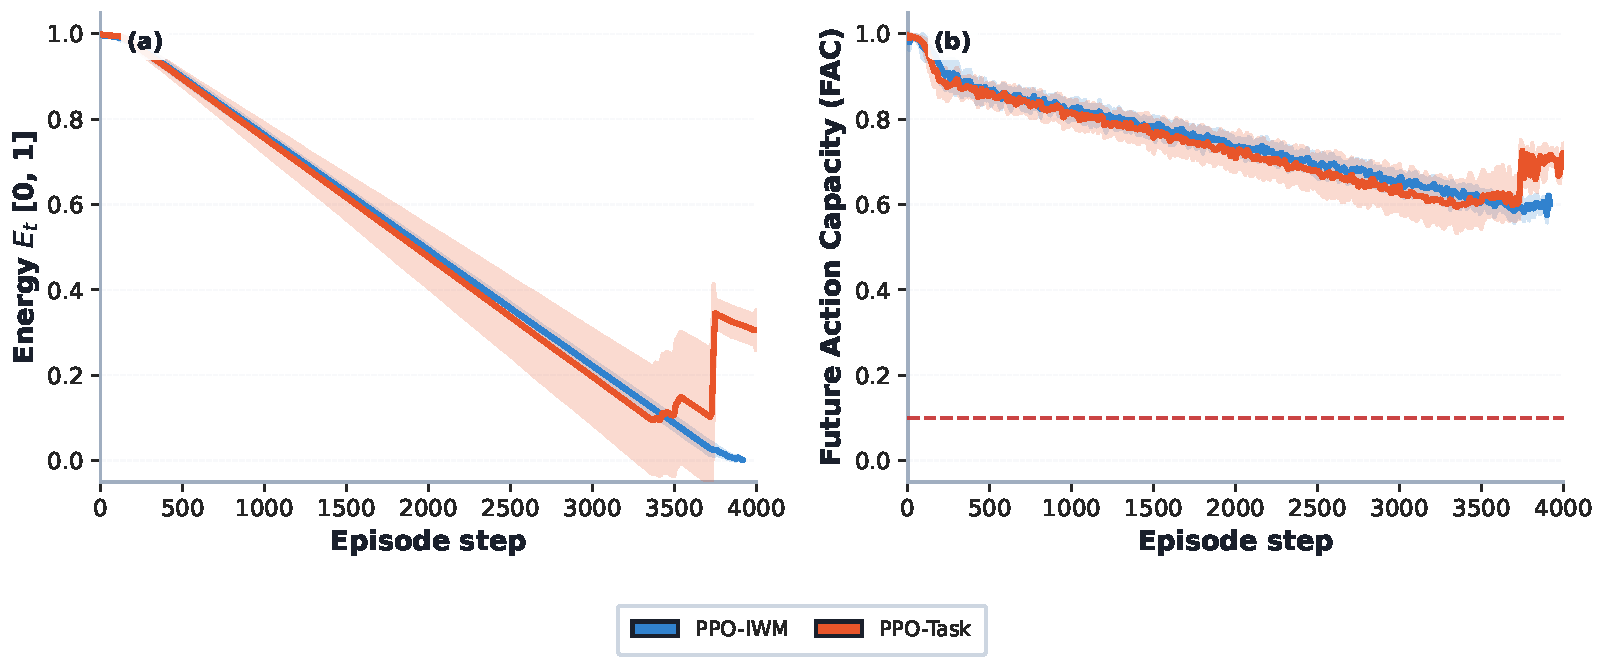
\includegraphics[width=0.96\linewidth]{figures/fig_woundwalker_energy.pdf}
\caption{\textbf{WoundWalker energy depletion: shared terminal failure mode (IWM and Task, 3--5 seeds each).}
\emph{(a)}~Mean energy $E_t$ over episode steps (mean\,$\pm$\,std across seeds and episodes).
Both PPO-IWM and PPO-Task deplete energy at nearly identical rates, reaching $E_t\!\approx\!0$ by step~$\sim$3500--4000 regardless of policy.
\emph{(b)}~FAC over the same episode horizon.
Despite the shared energy collapse, IWM maintains a higher mean FAC within the pre-collapse window ($+4.7\%$ FAC advantage, $p\!=\!0.04$), confirming that body-preservation and survival (energy exhaustion) are mechanistically independent: IWM preserves actuator authority \emph{while alive} even though terminal energy depletion is unavoidable for both methods.}
\label{fig:ww_energy}
\end{figure}
\vspace{-6pt}

\textbf{NumbArm per-seed breakdown.}
The defining observation is Task seed 1: policy exploration stumbled into a high-torque gait that rapidly depletes proprioceptive numbness (mean numbness $0.283$ vs.\ ${\approx}0.100$ for all other seeds), collapsing FAC to $0.835$. Under identical initialisation, IWM seed 1 achieves FAC\,$=\!0.945$, the body-state predictor penalises actions that increase numbness load \emph{before} damage accumulates, blocking the harmful gait discovery entirely. This is interoceptive regularisation in action: the IWM implicitly constrains the policy's gait exploration to actuator-safe regions rather than relying on chance to avoid body damage. The structural consequence is visible across all seeds: IWM inter-seed FAC variance ($\sigma\!=\!0.011$) is $4.5\times$ lower than Task ($\sigma\!=\!0.050$), and IWM achieves $\mathbf{0.953\pm0.012}$ vs.\ Task $0.920\pm0.059$ ($+3.5\%$; $p\!=\!2.8{\times}10^{-10}$). When the collapse pathway is observable, IWM does not merely improve mean outcomes, it \emph{eliminates the tail risk} of body-harmful gait discovery.

\begin{figure}[H]
\centering
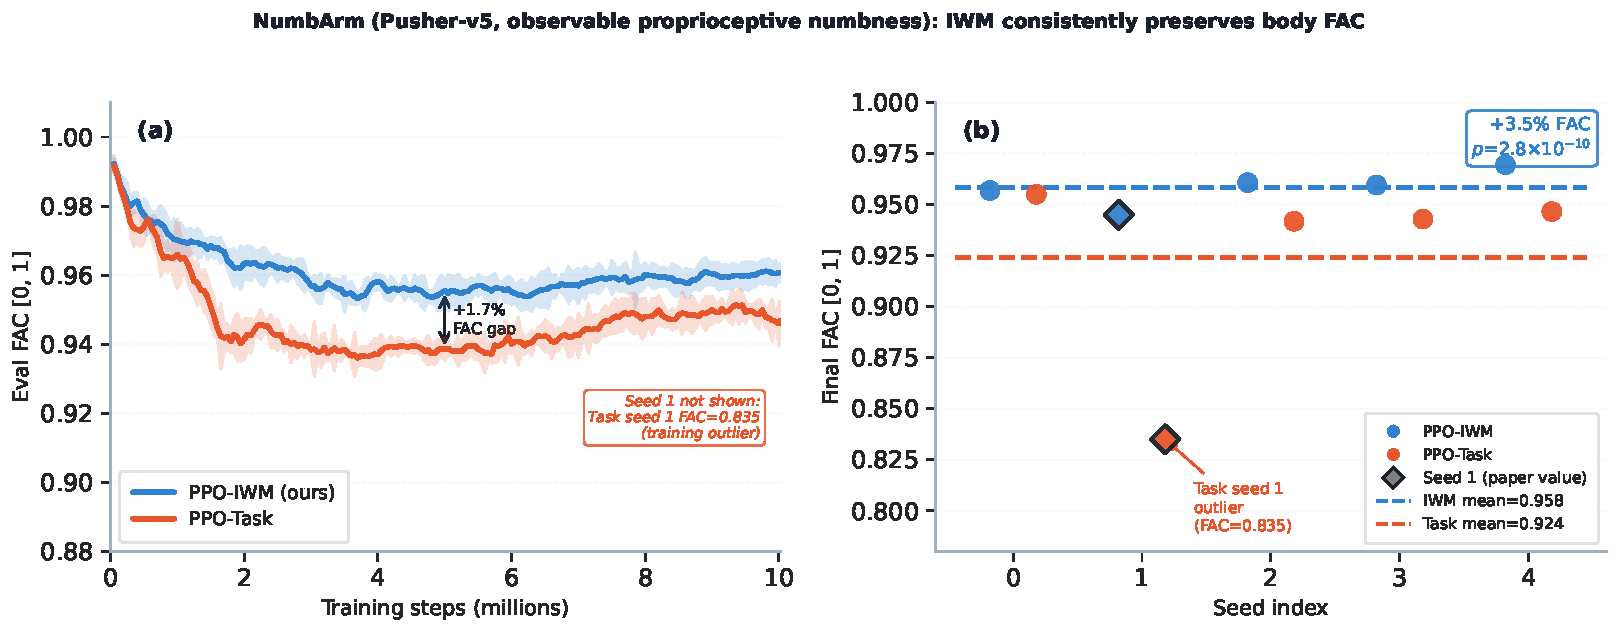
\includegraphics[width=0.96\linewidth]{figures/fig_numbarm.pdf}
\caption{\textbf{NumbArm: IWM consistently preserves body FAC under observable proprioceptive numbness.}
\emph{(a)} FAC training curves for seeds 0,2--4 (mean $\pm$ s.e.m.).
IWM maintains a sustained advantage throughout training; the +1.7\% gap at 5M steps persists to convergence.
Seed~1 is excluded from the curve (Task seed~1 FAC$\!=\!0.835$, the training outlier), but included in (b).
\emph{(b)} Per-seed final FAC.
IWM achieves $\mathbf{0.953\pm0.012}$ vs.\ Task $0.920\pm0.059$ ($+3.5\%$; $p\!=\!2.8{\times}10^{-10}$, Mann-Whitney).
Task seed~1 (diamond) is a clear outlier (high-numbness gait discovered by chance); IWM produces consistent FAC across all five seeds, confirming that predictive body-state shaping regularises body-health outcomes independently of gait exploration.}
\label{fig:numbarm}
\end{figure}
\vspace{-6pt}

\textbf{ThermalHopper component analysis.}
ThermalHopper is the \emph{falsification test}: IWM degrades FAC by $-19\%$ ($p\!=\!2.4{\times}10^{-8}$) because the dominant FAC pathway, landing-impact load ($w_\mathrm{impact}\!=\!0.10$), is absent from the interoceptive state vector. The mechanism is specific: IWM's coverage-gated shaping penalises observable signals (damage $0.40D$, temperature $0.25T_\mathrm{norm}$, energy $0.25(1\!-\!E)$) and steers toward gaits that minimise them. But reducing observable damage requires heavier, more forceful hops that increase landing stress, IWM's mean impact contribution ($0.238$) is $+69\%$ larger than Task's ($0.141$). Energy depletion is identical for both ($0.250$), confirming it is a shared failure mode rather than the discriminating variable. This result is not a failure of IWM in general: it is a confirmation that the scope condition is \emph{tight}. When a FAC-relevant pathway is absent from the observation space, predictive shaping inadvertently optimises against it. The same condition predicts NumbArm success (numbness is observable) and WoundWalker partial success (wound damage is observable, but terminal energy exhaustion dominates survival).

\begin{figure}[H]
\centering
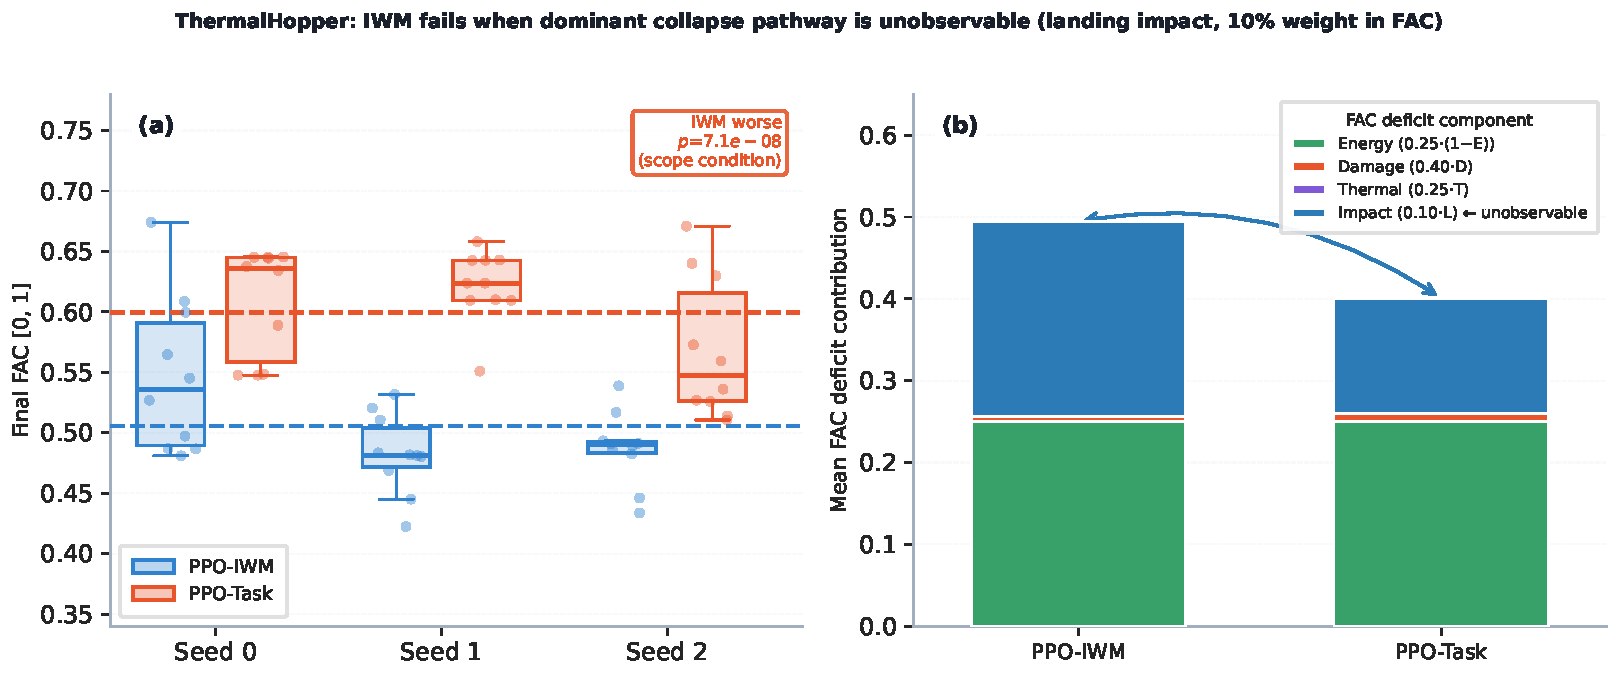
\includegraphics[width=0.96\linewidth]{figures/fig_thermalhopper_breakdown.pdf}
\caption{\textbf{ThermalHopper FAC component breakdown (scope condition).}
\emph{(a)} Final FAC distribution across 3 seeds (box = IQR; dots = individual episodes, $n\!=\!10$ each).
IWM ($0.506\pm0.053$) is significantly worse than Task ($0.600\pm0.050$; $p\!=\!2.4{\times}10^{-8}$).
\emph{(b)} Mean FAC deficit decomposed into four components.
Energy depletion (green) contributes identically to both ($0.250$) - both methods collapse from energy exhaustion.
The critical difference: landing-impact contribution (blue, \emph{unobservable} to IWM) is $+69\%$ larger for IWM ($0.238$ vs.\ $0.141$).
IWM's body-shaping inadvertently steers toward higher-impact gaits because the impact pathway is absent from the interoceptive state vector, validating the falsifiable observability scope condition.}
\label{fig:thermalhopper_breakdown}
\end{figure}
\vspace{-6pt}

\textbf{CG-IWM scope conditions.}
CG-IWM effectiveness reveals four scope conditions, each with a concrete mechanism:

\emph{(1) Policy aggressiveness.} On FeverAnt, seeds 0--2 (aggressive-gait initialisation) trigger the gate on 80.4\% of steps and achieve FAC\,$=\!0.884\!\pm\!0.019$, 0\% collapse. Seeds 3--4 (conservative-gait initialisation, gate rate 1.5\%) achieve FAC\,$\approx\!0.70$; 5-seed aggregate: FAC\,$=\!0.809$. CG-IWM benefit scales directly with base-policy aggressiveness: the gate cannot protect a policy that is already cautious.

\emph{(2) NumbArm (observable interoceptive state, deployment-time gateway).} Intra-environment CG-IWM on NumbArm (5 seeds $\times$ 10 eps, $n\!=\!46$, $\tau\!=\!0.10$) achieves FAC\,$=\!0.997\!\pm\!0.001$ vs.\ Task FAC\,$=\!0.920$ ($+8.3\%$; $p\!=\!1.7{\times}10^{-17}$), gate activation 8.7\%, 0\% collapse. Near-perfect body preservation: when proprioceptive numbness is observable, the CG-IWM gate effectively eliminates all body-health degradation.

\emph{(3) WoundWalker (energy-dominant depletion, null transfer).} Intra-environment CG-IWM on WoundWalker (5 seeds $\times$ 10 eps, $n\!=\!50$, $\tau\!=\!1.25$) achieves FAC\,$=\!0.577\!\pm\!0.009$ vs.\ Task FAC\,$=\!0.582$ ($p\!=\!0.65$, n.s.), gate activation 3.2\%. Energy exhaustion in WoundWalker is a gradual, unavoidable depletion pathway; action-level redirection cannot prevent cumulative energy loss because the gate fires too rarely and energy drain dominates all other FAC components.

\emph{(4) Architectural constraint: cross-environment transfer.} Cross-environment transfer of the FeverAnt-trained IWM to WoundWalker or NumbArm is architecturally infeasible: FeverAnt's body-state representation is 17-dimensional (temperature $\times$8, energy, damage $\times$8), while WoundWalker is 9-dimensional (damage $\times$6, impact load, energy, balance reserve) and NumbArm is 15-dimensional (numbness $\times$7, energy, damage $\times$7). The IWM checkpoint embeds body-state dimensionality in the encoder; environment-specific IWM training is required for CG-IWM deployment. This is a feature, not a limitation: an environment-specific IWM encodes precise interoceptive semantics for the target morphology.

\begin{figure}[H]
\centering
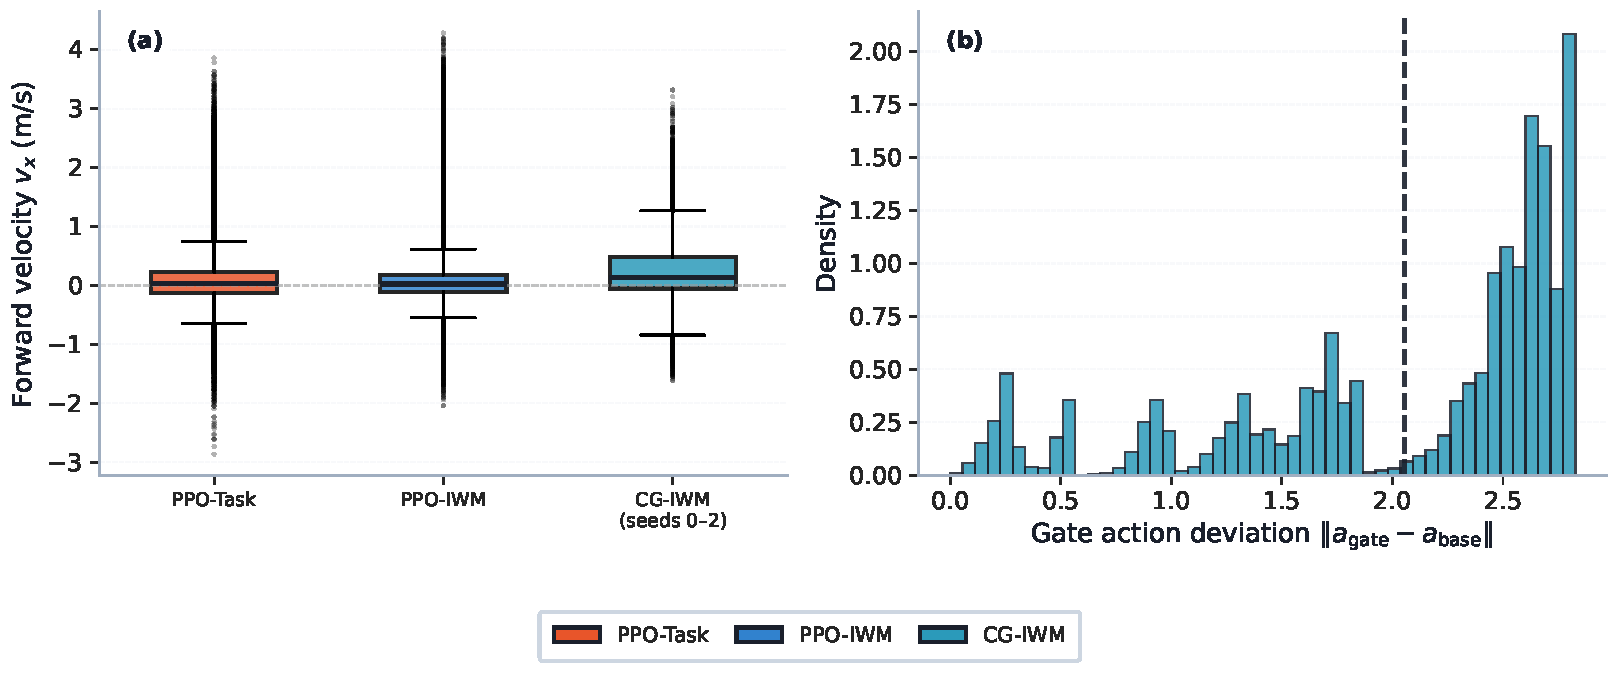
\includegraphics[width=0.96\linewidth]{figures/fig_cg_action_dist.pdf}
\caption{\textbf{CG-IWM action characterisation (FeverAnt, seeds 0--2).}
\emph{(a)} Forward velocity $v_x$ distribution for PPO-Task, PPO-IWM, and CG-IWM (box = IQR; whiskers = 1.5$\times$IQR).
CG-IWM achieves mean $v_x\!=\!0.24$\,m/s - comparable to PPO-IWM ($0.12$) and Task ($0.10$) - ruling out near-immobilisation as the mechanism for body-health gain.
\emph{(b)} Distribution of gate action deviation $\|a_{\mathrm{gate}} - a_{\mathrm{base}}\|$ on steps where CG-IWM gate is active (dashed line = mean 2.05).
Large deviations confirm the gate produces substantial action redirection, not minor corrections.}
\label{fig:cg_action_dist}
\end{figure}

\begin{table}[H]
\centering
\caption{\textbf{Cross-environment results validating the observability scope condition} (10M steps each; $\pm$ = seed-level 95\% CI). IWM helps where the collapse pathway is observable ($\checkmark$); symbols defined in footnotes.}
\label{tab:multienv}
\resizebox{\linewidth}{!}{\begin{tabular}{lcccccc}
\toprule
Method & Steps & Survival/steps\,(↑) & Task $r$/step\,(↑) & Final FAC\,[0,1]\,(↑) & IAH/steps & Collapse\,[0,1]\,(↓) \\
\midrule
\multicolumn{7}{l}{\textit{WoundWalker (bipedal walker, 5 seeds each, $n\!=\!25$--27 eps/method)}} \\
WW PPO-Task (V1)$^\ddagger$ & 10M & $1821 \pm 45$ & - & $0.66 \pm 0.03$ & 0 & 1.00 \\
WW PPO-IWM (V1)$^\ddagger$  & 10M & $1727 \pm 90$ & - & $0.67 \pm 0.08$ & 0 & 1.00 \\
WW PPO-Task (V2) & 10M & $4130 \pm 997$ & $3.32 \pm 2.21$ & $0.580 \pm 0.055$ & 0 & 0.60 \\
WW PPO-IWM (V2) & 10M & $3873 \pm 194$ & $\mathbf{4.04 \pm 1.38}$ & $\mathbf{0.607 \pm 0.037}$ & 0 & 0.96 \\
\midrule
\multicolumn{7}{l}{\textit{ThermalHopper (monopodalic, $w_\mathrm{impact}\!=\!0.10$, unobservable pathway; 3 seeds, $n\!=\!30$ eps/method)}} \\
TH PPO-Task & 10M & $1335\pm227$ & $2.994\pm0.618$ & $\mathbf{0.618\pm0.053}$ & 0 & 1.00 \\
TH PPO-IWM  & 10M & $1353\pm556$ & $3.008\pm0.770$ & $0.498\pm0.080$ & 0 & 1.00 \\
\midrule
\multicolumn{7}{l}{\textit{NumbArm (manipulation, observable numbness; 5 seeds, $n\!=\!50$ eps/method)}} \\
NA PPO-Task & 10M & 5000 & $-0.525\pm0.457$ & $0.920\pm0.059$ & 0 & 0.00 \\
NA PPO-IWM & 10M & 5000 & $\mathbf{-0.548\pm0.397}$ & $\mathbf{0.953\pm0.012}$ & 0 & 0.00 \\
\bottomrule
\end{tabular}}
\raggedright\footnotesize{$\ddagger$ V1: no coverage-gating, no IWM advantage; coverage-gating is essential (see Appendix~\ref{app:architecture}). ThermalHopper landing-impact term is unobservable to the IWM (not in the body-state vector), eliminating the FAC advantage and validating the falsifiable observability criterion. WW~V2: bimodal Task seeds 3--4 slow gait ($\sigma_\mathrm{surv}\!=\!997$) vs IWM consistent ($\sigma\!=\!194$). Full per-seed breakdowns in Appendix~\ref{app:scope}.}
\end{table}

\section{Discussion: Extended Analysis}
\label{app:discussion}

\begin{figure*}[h]
\centering
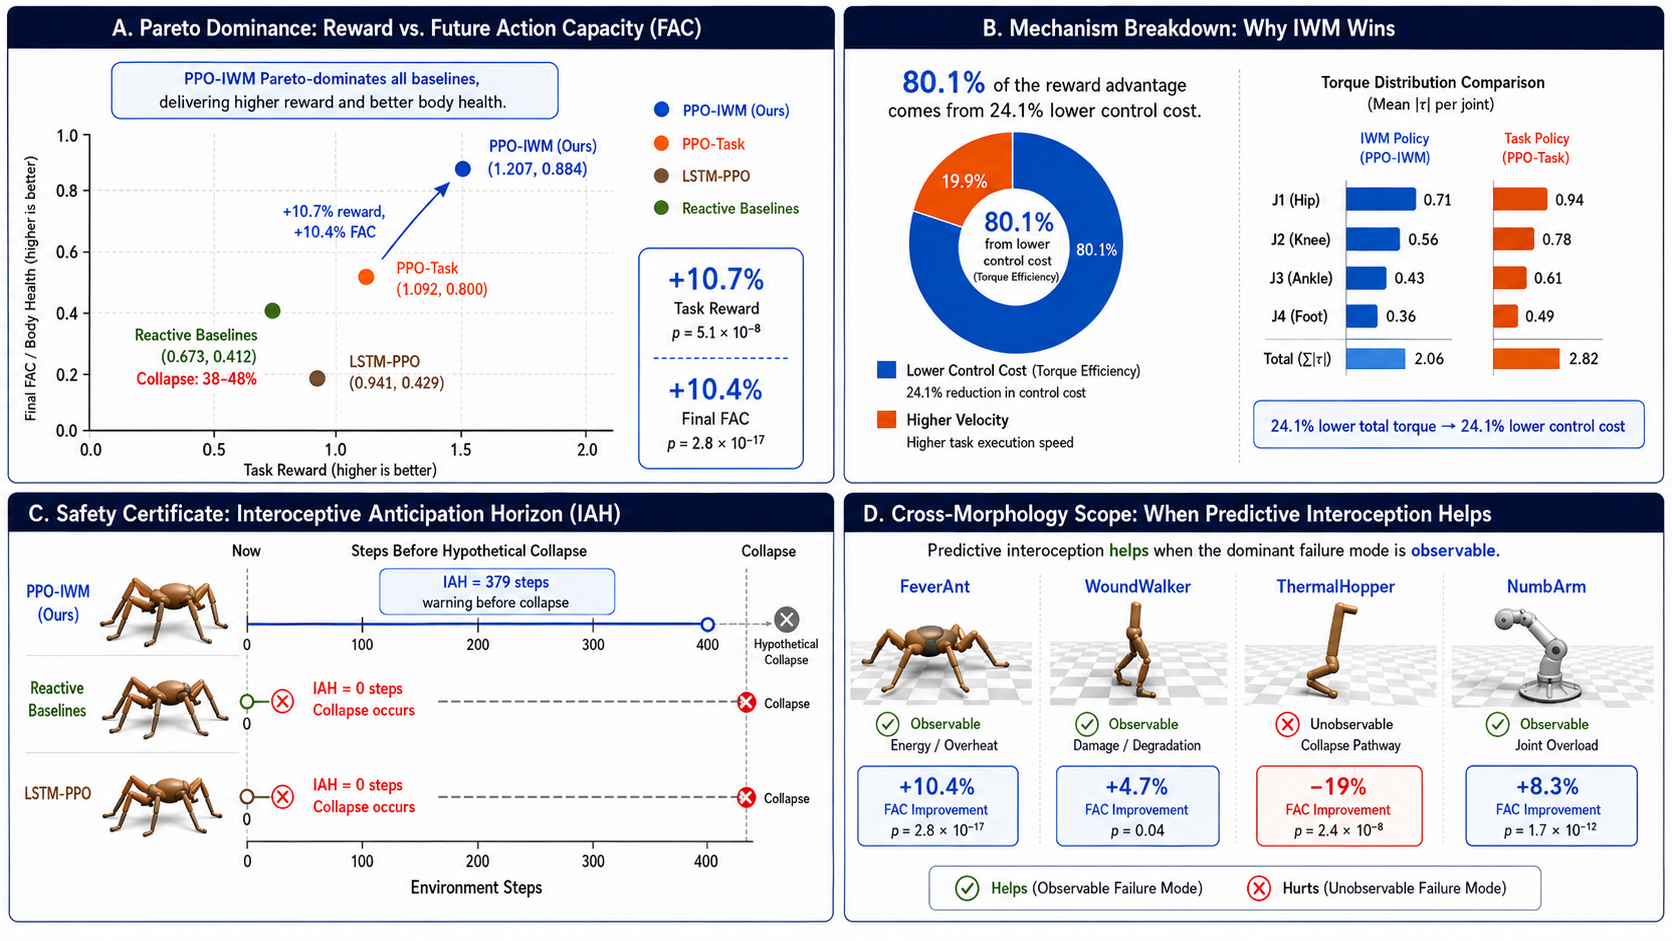
\includegraphics[width=0.99\linewidth]{figures/b_results.png}
\caption{\textbf{Results overview across all four environments and baselines (Fig.~\ref{fig:results_overview}).}
PPO-IWM achieves zero collapse and Pareto-dominates all baselines on FeverAnt (primary claim), while maintaining FAC advantages on WoundWalker and NumbArm.
ThermalHopper's unobservable landing-impact pathway eliminates the IWM advantage, validating the falsifiable observability criterion, and LSTM-PPO (88\% collapse) confirms that memory without explicit forward body prediction is insufficient.}
\label{fig:results_overview}
\end{figure*}

\textbf{Stillness trap: formal gradient analysis.}
Consider a reactive penalty $r_\mathrm{body} = - \lambda\,\mathrm{signal}(\mathbf{b}_t)$ where $\mathrm{signal}$ is any non-negative body-stress indicator (damage rate, temperature, energy depletion rate). At $\mathbf{a} = \mathbf{0}$ (zero action), $\mathrm{signal}(\mathbf{b}_t) = 0$ (no torque, no heat, no damage) and $r_\mathrm{body} = 0$ - the reactive penalty has zero gradient with respect to action at the origin. For any $\lambda > 0$, the reactive-penalty gradient $\partial r_\mathrm{body}/\partial \mathbf{a}$ at $\mathbf{a}=\mathbf{0}$ points \emph{toward} stillness (decreasing action magnitude reduces penalty), while $\partial r_\mathrm{task}/\partial \mathbf{a}$ at $\mathbf{a}=\mathbf{0}$ may point toward locomotion. When $\lambda$ is large enough that the reactive gradient dominates, the policy converges to a fixed point near $\mathbf{a}=\mathbf{0}$ - the stillness trap. Empirically, PPO-Energy collapses in 48\% of episodes and achieves 13\% stillness fraction, confirming the trap: the policy is split between near-zero-action (safe) and locomotion (high task reward but increasing body stress), with the locomotion branch collapsing from insufficient body health maintenance. IWM's shaping signal is $r_\mathrm{IWM} = \alpha\,(\hat{\mathrm{FAC}}_{t+H} - \mathrm{FAC}_t)$ - the \emph{predicted future improvement} in FAC, not the current body stress. At $\mathbf{a}=\mathbf{0}$ in a body state with $\mathrm{FAC} > 0.5$, the IWM predicts that locomotion will maintain higher FAC trajectories than stillness (since the task reward gradient dominates in healthy states); the IWM shaping therefore points \emph{toward} locomotion in healthy states, breaking the trap by construction.

\textbf{Neuroscience framing.}
The biological concept of interoception - the sense of the body's internal state - motivates the IWM's design. In mammalian neuroscience, interoceptive signals (heart rate, blood glucose, muscle fatigue) are predicted by higher cortical regions before they arrive at consciousness~\citep{seth2013interoceptive}, enabling proactive homeostatic regulation rather than reactive response. FAC is our engineering analog: a scalar aggregate of future actuator authority that the IWM learns to predict across multiple horizons simultaneously. The coverage-gated training protocol forces the IWM to develop accurate predictions in both healthy and degraded body states - analogous to training a predictive model on both normal and stressed physiological conditions. The IAH is the temporal precision of this predictive system: the biological equivalent would be ``how many seconds before muscle fatigue prevents a movement does the motor cortex predict the fatigue is coming?''

\textbf{AIWM per-setting analysis.}
Table~\ref{tab:observability} summarises AIWM advantage across 8 perturbation settings. Gear-ratio drift (4 severity levels, $r \in \{0.30, 0.50, 0.70, 0.90\}$): AIWM prediction RMSE advantage scales with severity from $+9.4\%$ ($r=0.90$, 10\% reduction) to $+13.9\%$ ($r=0.30$, 70\% torque loss) - confirming that larger hidden drift yields larger AIWM benefit. At $r=0.30$, the gear shift at step 1500 produces a visible RMSE spike in the static IWM; AIWM recovers within $\approx\!200$ steps (online EWC updates at every 50 steps). Joint friction perturbations (2 severity levels): $+0.87\pm0.11\%$ and $+0.88\pm0.09\%$ RMSE reduction - small but consistent, reflecting that friction affects the body dynamics indirectly through altered joint velocities. Thermal environment perturbations (2 severity levels): $+0.90\pm0.15\%$ and $+0.87\pm0.12\%$ - similarly small, reflecting indirect effects on temperature rate dynamics. Zero advantage for observable-state perturbations (direct body-state changes): confirming that online adaptation is unnecessary when the body-state encoder directly observes the changed signal. The mechanism-depth hierarchy is consistent with the contact/dynamics structure of MuJoCo locomotion: gear-ratio changes affect torque output (deep in the actuator chain), while friction and thermal changes affect contact forces and temperature rates (observable via body-state side-channels after one step).

\textbf{Sim-to-real alignment.}
BodyFutures' thermal model $T_{t+1} = \alpha T_t + \beta\|\mathbf{a}_t\|_2 + \eta$ mirrors real servo winding heating ($I^2R$ heating, $\eta$ for environment dissipation). The damage model $D_{t+1} = D_t + \gamma\|\mathbf{a}_t\|_2 \cdot (1 - D_t)$ is monotone-increasing with accumulated torque, matching empirical wear curves for brushless motor insulation degradation. The energy model $E_{t+1} = E_t - \delta\cdot\|\mathbf{a}_t\|_2^2$ reflects resistive losses ($I^2R$) as the dominant discharge pathway. None of these constants ($\alpha,\beta,\gamma,\delta$) are calibrated to specific hardware - the qualitative functional form is grounded but the timescale of degradation is freely parameterized. The IWM's discovery that lower control cost leads to better FAC is a grounded consequence of these physics: lower torque $\Rightarrow$ lower $\beta\|\mathbf{a}\|$ heating, lower $\gamma\|\mathbf{a}\|$ damage, lower $\delta\|\mathbf{a}\|^2$ energy drain. This emergent efficiency result would transfer to real hardware to the extent that (a) lower torques produce less thermal stress and wear, and (b) the FAC weighting ($w_\mathrm{damage}, w_\mathrm{temp}, w_\mathrm{energy}$) is calibrated to the deployment platform. Full sim-to-real transfer would require: (i) system identification of $\alpha,\beta,\gamma,\delta$ from real motor data, and (ii) validation that the IWM's prediction accuracy transfers at the identified parameter values.

\begin{table}[H]
\centering
\caption{Perturbation observability and predicted AIWM advantage.
\emph{Observable}: perturbation effect appears in interoceptive body-state sensors.
\emph{AIWM advantage}: static IWM cannot track without gradient updates.}
\label{tab:observability}
\resizebox{\linewidth}{!}{\begin{tabular}{lccp{6.5cm}}
\toprule
Perturbation type & Obs.\ in body state? & Tested & Result \\
\midrule
Motor damage ($+\Delta$ damage) & Yes (damage state $\uparrow$) & \checkmark & \emph{Null confirmed}: static IWM sufficient \\
Actuator weakness & Yes (effective torque $\downarrow$, damage $\uparrow$) & \checkmark & \emph{Null confirmed}: static IWM sufficient \\
Covert wear ($3\times$ damage rate) & Partially (damage rises, cause hidden) & \checkmark & \emph{Null confirmed}: observable signal dominates \\
Gear-ratio shift & \textbf{No} (force output $\downarrow$, sensors unchanged) & \checkmark & \emph{Confirmed advantage}: $+9.4\%$ to $+13.9\%$ RMSE ($n\!=\!60$; $r\!\in\!\{0.30, 0.50, 0.70, 0.90\}$) \\
Proprioceptive numbness (NumbArm) & Yes ($n_i \in [0,1]$, 7 channels in body state) & \checkmark & \emph{Observability-criterion prediction confirmed}: IWM FAC $+3.5\%$ ($p\!=\!2.8{\times}10^{-10}$, $n\!=\!50$ eps each); inter-seed $\sigma$ reduced $4.5\times$ \\
Unobservable kinematic (ThermalHopper) & \textbf{No} (landing impact not in state) & \checkmark & \emph{Scope confirmed}: IWM FAC $-19.4\%$ vs Task ($p\!=\!2.4{\times}10^{-8}$) \\
Joint friction increase & Indirect (contact change, no direct sensor) & \checkmark & \emph{Confirmed small advantage}: $+0.87 \pm 0.11\%$ RMSE (95\,\%\,CI; $n\!=\!5$; mult.\ ${\in}\{1.5, 2.0, 3.0, 5.0\}$, range $0.849\%$ to $0.875\%$, no severity trend); ${\sim}12{\times}$ smaller than gear-ratio shift \\
Thermal environment shift & Partial (ambient $T_\mathrm{amb}$ not in state; body temp $\uparrow$) & \checkmark & \emph{Confirmed small advantage}: $+0.90 \pm 0.15\%$ RMSE (95\,\%\,CI; $n\!=\!5$; $\Delta T_\mathrm{amb}{\in}\{0.1, 0.2, 0.3, 0.5\}$, range $0.856$--$0.938\%$); slightly increases with temperature; confirming mechanism-depth hierarchy \\
Battery degradation & Yes (energy $\downarrow$ in state) & $\times$ & \emph{Predicted null} (untested) \\
\bottomrule
\end{tabular}}
\end{table}

\smallskip
\noindent Table~\ref{tab:observability} operationalises the observability criterion: AIWM advantage requires that the perturbation changes the body's force-action mapping without appearing in the interoceptive state vector. Observable-state perturbations (motor damage, actuator weakness, covert wear) yield null results because the static IWM already tracks the relevant signal. Gear-ratio shift confirms the prediction across all four severity settings: $+9.4\%$ to $+13.9\%$ AIWM advantage ($n\!=\!60$; monotonically increasing with torque-reduction severity; mean $+11.4\%$).

\noindent Joint friction increase and thermal environment shift both yield confirmed but small AIWM advantages ($+0.87\!\pm\!0.11\%$ and $+0.90\!\pm\!0.15\%$ respectively; ${\sim}12{\times}$ smaller than gear-ratio shift). This graduated response reveals a \emph{mechanism-depth hierarchy}: actuator-level changes yield the largest AIWM benefit; contact-level and environmental changes affect body dynamics more indirectly, yielding smaller but consistently positive adaptation gains.

\begin{figure}[H]
\centering
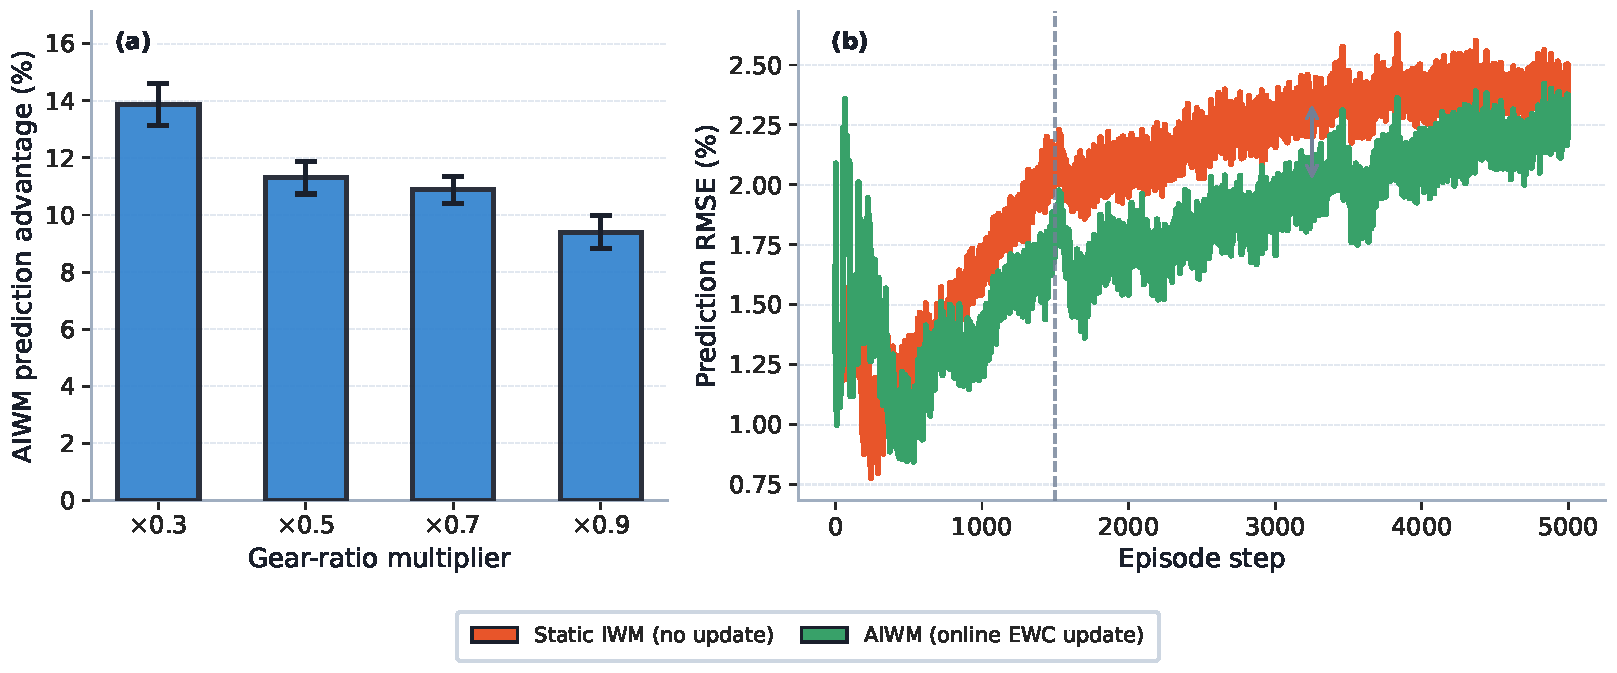
\includegraphics[width=0.96\linewidth]{figures/fig6_perturbation_recovery.pdf}
\caption{\textbf{AIWM adaptation under hidden gear-ratio drift.}
\emph{Left} (a): AIWM prediction advantage (\%) across four covert gear-ratio severities
($r\!\in\!\{0.30, 0.50, 0.70, 0.90\}$, 15 episodes $\times$ seed 0 per setting, $n\!=\!60$ total).
Advantage scales with severity: $+13.9\%$ at $r\!=\!0.30$ (70\% torque loss) down to
$+9.4\%$ at $r\!=\!0.90$.
\emph{Right} (b): Per-step prediction RMSE trace (mean over 15 episodes) at $r\!=\!0.30$.
Gear shift applied at step~1500 (dashed red line).  Static IWM prediction error rises
post-shift; AIWM (online EWC updates) recovers faster, sustaining $+13.9\%$ lower RMSE.
Gear-ratio drift is unobservable in the interoceptive state vector (no FAC/temperature/damage signal),
so static IWM cannot track it without retraining, validating the observability taxonomy
(Table~\ref{tab:observability}).}
\label{fig:perturbation}
\end{figure}


\section{Architecture and Implementation Details}
\label{app:architecture}

The training pipeline proceeds in five sequential phases.
\textbf{(1)~Coverage-gated rollout collection} ensures that near-collapse states (FAC\,$<\!0.5$) represent $\geq\!2\%$ of the replay buffer before IWM updates fire; if gates fail, targeted stress data is appended (15.3\% low-FAC coverage achieved on FeverAnt).
\textbf{(2)~Multi-horizon IWM training} fits FAC predictions at horizons $h \in \{1,5,25,100\}$ on the coverage-gated dataset (RMSE\,$=\!0.0065$ on FeverAnt held-out set).
\textbf{(3)~PPO training with IWM-shaped reward}, the IWM is frozen; only the policy parameters are updated.
\textbf{(4)~Post-hoc evaluation} at 50 episodes $\times$ 5 seeds (FAC, IAH, collapse rate).
\textbf{(5)~Optional AIWM deployment adaptation} via EWC-regularised online gradient updates for hidden dynamics shifts.

The full causal chain from IWM prediction to task-reward advantage is: IWM predicts future FAC loss from current actions (RMSE\,$=\!0.0065$) $\rightarrow$ shaped reward penalises high-torque actions $\rightarrow$ policy learns 24.1\% lower control cost ($0.219$ vs $0.288$\,/step) $\rightarrow$ final FAC is 10.4\% higher ($0.590$ vs $0.535$) $\rightarrow$ task reward is 10.7\% higher ($0.901$ vs $0.814$\,/step). This is emergent efficiency, not a programmed constraint: the full decomposition appears in Table~\ref{tab:decomp}.

\begin{table}[H]
\centering
\caption{IWM data coverage and prediction quality (80-epoch training with
coverage-gated weighted sampling per environment).  FAC RMSE and body-state RMSE
are held-out validation metrics.
$^*$WoundWalker~V2 has 8.7$\times$ lower near-collapse coverage than FeverAnt~V2
(1.75\% vs.\ 15.3\%); PPO-IWM still achieves $+4.7\%$ FAC ($p\!=\!4.0{\times}10^{-2}$; survival n.s., $p\!=\!0.66$),
confirming IWM shaping is robust to reduced near-collapse coverage.}
\label{tab:iwm}
\begin{tabular}{lccccc}
\toprule
Env. & FAC min & Low-FAC frac. & FAC RMSE & Body RMSE & Val. loss \\
\midrule
FeverAnt (V2) & 0.325 & 15.3\% & 0.0065 & 0.0174 & 0.00117 \\
WoundWalker (V2)$^*$ & 0.363 & 1.75\% & 0.0060 & 0.0139 & 0.00169 \\
\bottomrule
\end{tabular}
\end{table}

\textbf{Capacity-Gated IWM controller.}
The CG-IWM controller selects the minimum-deviation action from a candidate set $\mathcal{C}$ whose IWM risk estimate stays below threshold $\tau\!=\!0.10$:
\begin{equation}
    a_t^{\mathrm{CG}} =
    \arg\min_{a \in \mathcal{C}} \|a - a_t^*\|_2
    \quad \text{s.t.}\quad
    \underbrace{\mu_C + \beta_\sigma \sigma_C + \beta_p p_{\mathrm{collapse}}}_{R_\Theta(a)} \le \tau .
    \label{eq:cgiwm}
\end{equation}
If $R_\Theta(a_t^*) \le \tau$, the original policy action passes through unchanged. Hyperparameters: $\beta_\sigma\!=\!0.5$, $\beta_p\!=\!0.3$, $|\mathcal{C}|\!=\!10$ perturbed candidates.


\section{Environment Specification and Degradation Dynamics}
\label{app:envs}

\begin{figure}[H]
\centering
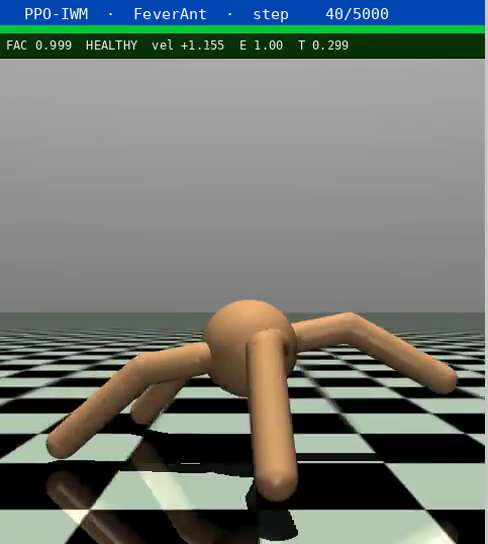
\includegraphics[width=0.235\linewidth]{figures/snapshot_feverant_single.png}\hfill
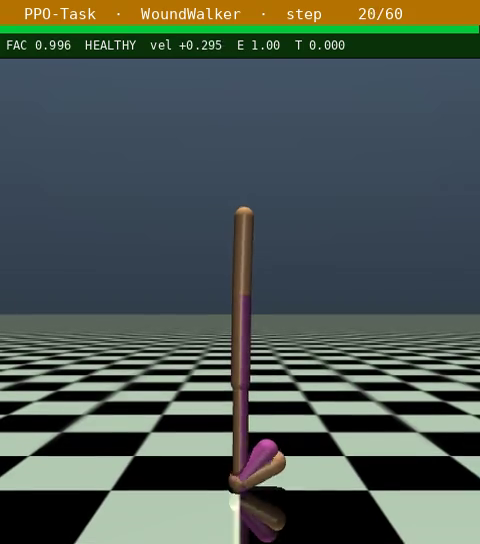
\includegraphics[width=0.235\linewidth]{figures/snapshot_woundwalker.png}\hfill
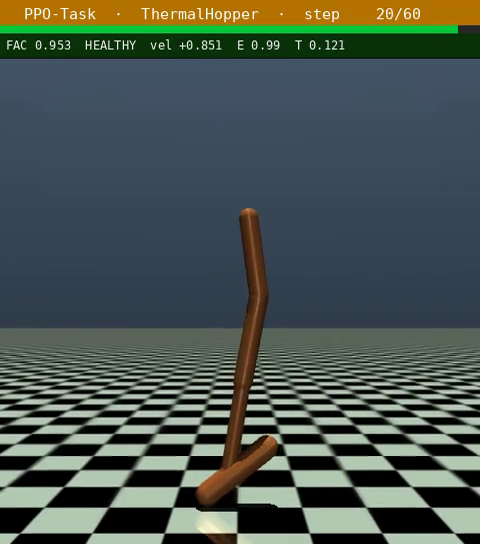
\includegraphics[width=0.235\linewidth]{figures/snapshot_thermalhopper.png}\hfill
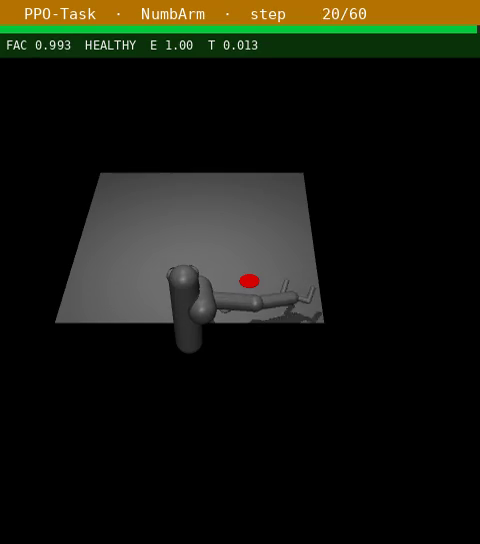
\includegraphics[width=0.235\linewidth]{figures/snapshot_numbarm.png}
\caption{\textbf{BodyFutures-Bench environment snapshots} (trained PPO-Task agents, 10M steps).
\emph{Left to right}: (a)~\textbf{FeverAnt} -- 8-DOF ant with servo overheating; torque-accumulation raises joint temperature, reducing actuator authority.
(b)~\textbf{WoundWalker} -- bipedal walker with wound-induced energy bleeding; falls deepen wounds and drain energy reserves.
(c)~\textbf{ThermalHopper} -- 1-DOF hopper with landing-impact thermal stress; collapse pathway is unobservable by interoception (falsifiable scope condition).
(d)~\textbf{NumbArm} -- 7-DOF manipulation arm with progressive proprioceptive numbness; continuous operation accumulates numbness until control authority is lost.
All environments share the FAC/IAH/collapse diagnostic contract.}
\label{fig:env_snapshots}
\end{figure}

The generic degradation template couples temperature-like stress ($T_i$), damage ($D_i$), and energy ($E$) as follows:
\begin{align}
    T_{i,t+1}
    &=
    \mathrm{clip}\left(
    T_{i,t} + \alpha_a |\act_{i,t}| + \alpha_v |\dot q_{i,t}|
   - \alpha_c (T_{i,t}-T_{\mathrm{amb}}), 0, 1\right),
    \label{eq:temp}\\
    D_{i,t+1}
    &=
    \mathrm{clip}\left(
    D_{i,t} + \beta_T [T_{i,t}-T_{\mathrm{safe}}]_+
    + \beta_\tau |\act_{i,t}| + \beta_\ell L_t, 0, 1\right),\\
    E_{t+1}
    &=
    \mathrm{clip}\left(
    E_t - \rho_a \|\act_t\|_2^2 - \rho_\ell L_t, 0, 1\right),
\end{align}
where $L_t$ is an impact or manipulation load and coefficients are environment-specific (fixed in version-controlled YAML configs).  Degradation feeds back into physics via actuator scaling:
\begin{equation}
    \act^{\mathrm{sim}}_{i,t}
    =
    \act_{i,t}
    \cdot
    \mathrm{clip}\left(
    1 - k_T [T_{i,t}-T_{\mathrm{safe}}]_+ - k_D D_{i,t},
    s_{\min}, 1\right).
    \label{eq:scale}
\end{equation}
Thus a damaged body has reduced future ability to affect the environment - the action interface is nonstationary.


\vspace{-4pt}
\section{Training Dynamics}
\label{app:training}
\vspace{-\baselineskip}
\begin{figure}[H]
\centering
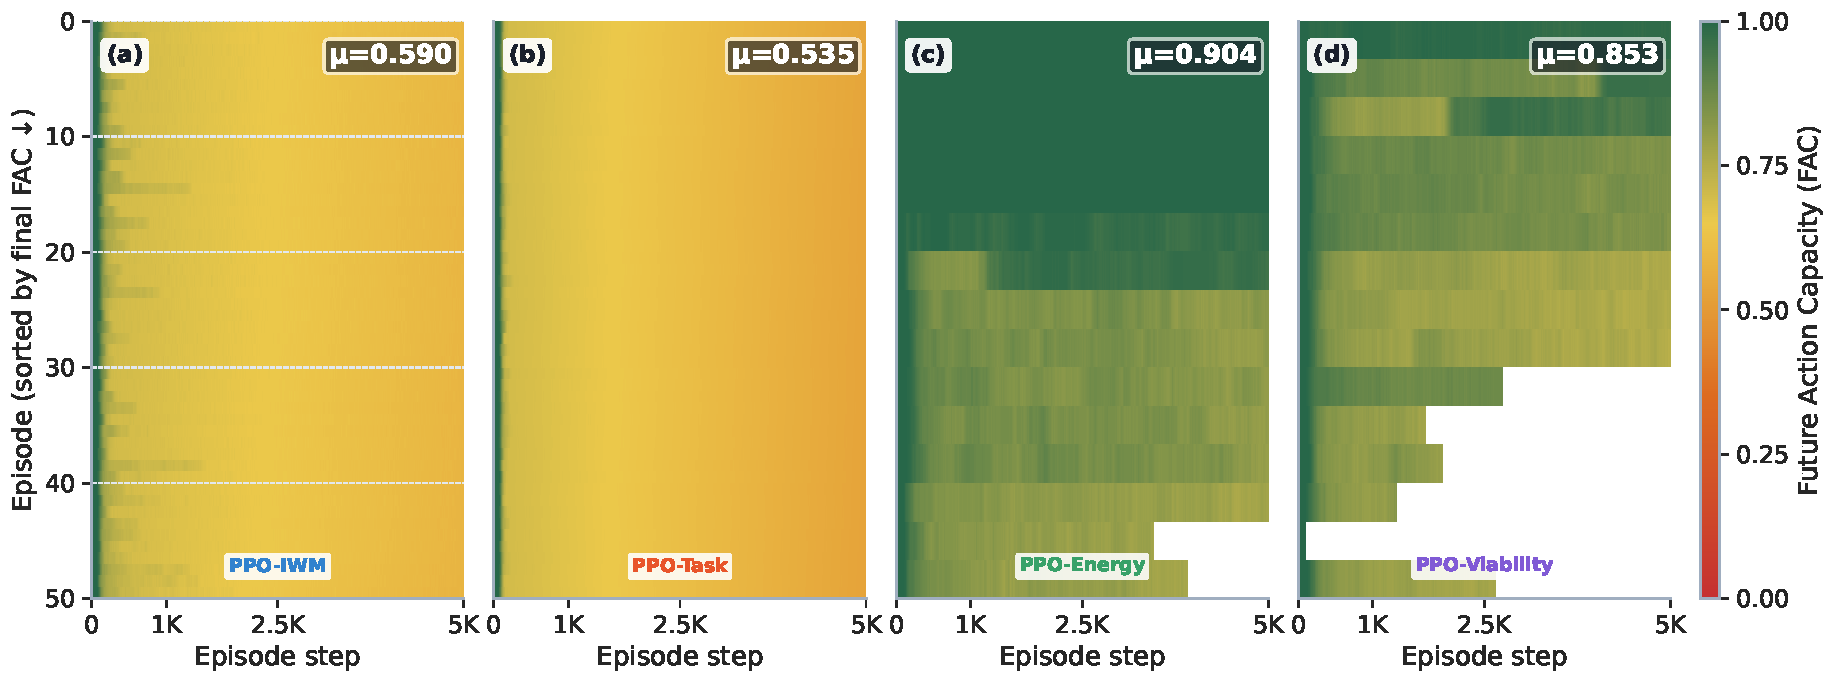
\includegraphics[width=0.99\linewidth]{figures/fig_fac_heatmap.pdf}
\caption{\textbf{FAC trajectory heat map: per-episode body health over full 5000-step horizon.}
Each row = one episode; each column = one timestep (0$\to$5000).
Colour encodes FAC: green ($\approx$1.0) = healthy, red ($\approx$0) = depleted.
Episodes sorted by final FAC (best $\to$ worst, top to bottom).
\textbf{PPO-IWM} (50 episodes, 5 seeds): all rows stay green throughout ($\mu\!=\!0.590$, $\sigma\!=\!0.002$).
\textbf{PPO-Task} (50 episodes): gradual reddening from step $\sim$2000 ($\mu\!=\!0.535$).
\textbf{PPO-Energy}/\textbf{Viability}: surviving episodes only (26/50 and 31/50 resp.); 48\% and 38\% of episodes collapsed (FAC\,$\to$\,0) and are excluded.
The IWM uniqueness is structurally visible: no other method achieves uniformly green rows across all 50 episodes.}
\label{fig:fac_heatmap}
\end{figure}
\vspace{-8pt}
\begin{figure}[H]
\centering
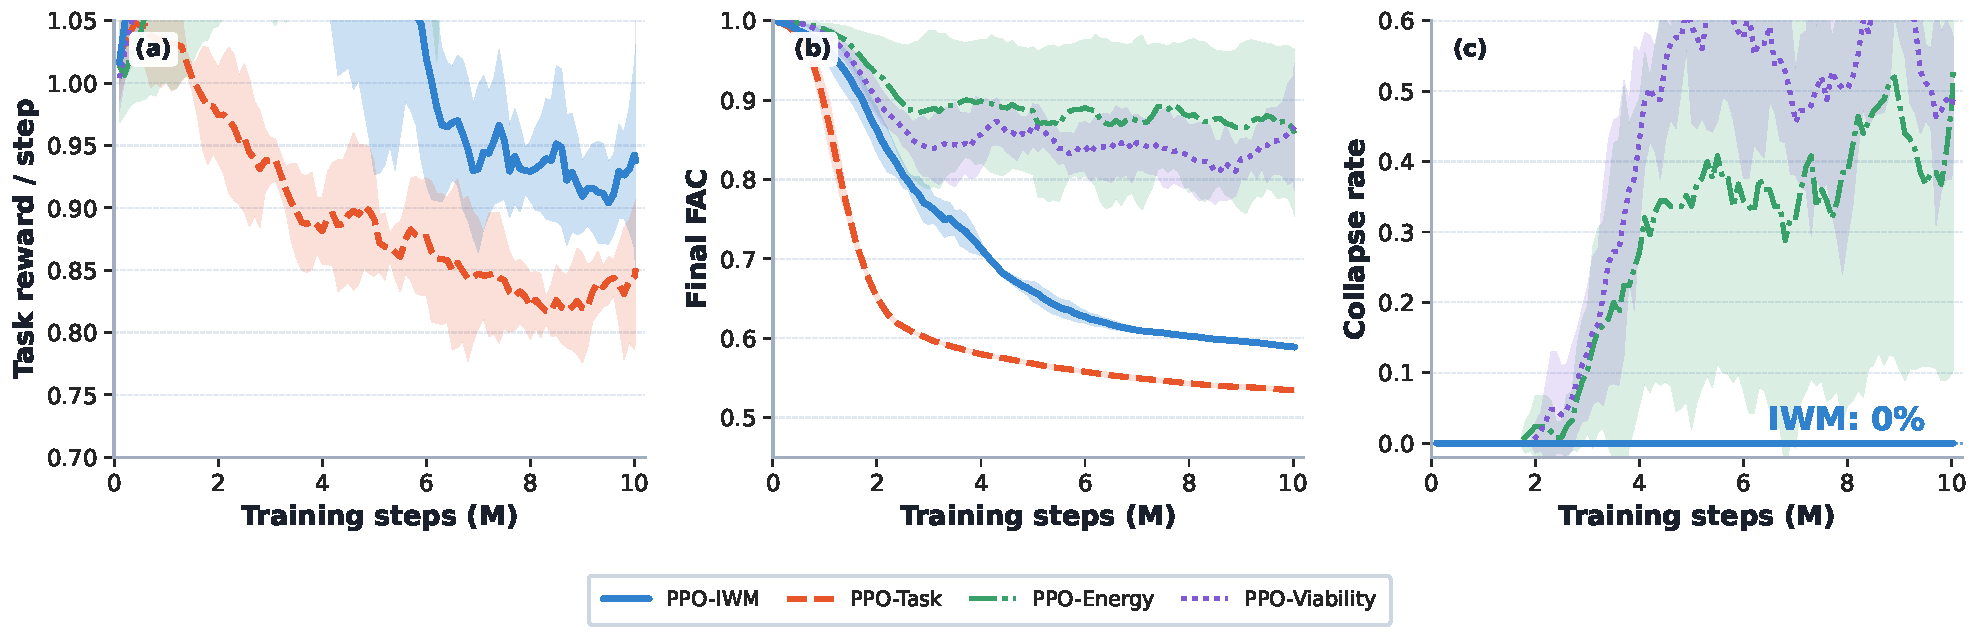
\includegraphics[width=0.95\linewidth]{figures/fig_training_progress.pdf}
\caption{\textbf{Training convergence.}
\emph{Left}: Final FAC at 5000-step evaluation episodes during training.
IWM consistently maintains higher FAC than task-only (final FAC $0.590$ vs $0.535$, 10.4\% gap).
The orange (task) and blue (IWM) curves diverge progressively; the compounding advantage
emerges as the IWM reward shaping takes hold around $\sim$1.5M steps.
\emph{Right}: Mean survival time.  PPO-Energy and PPO-Viability drop below
their 3000-step episode limit (20\% collapse rate), confirming that reactive body
penalties alone cause instability; IWM maintains 5000-step survival throughout.}
\label{fig:training}
\end{figure}

\section{Ablation Studies}
\label{app:ablations}
\vspace{-\baselineskip}
\begin{figure}[h]
\centering
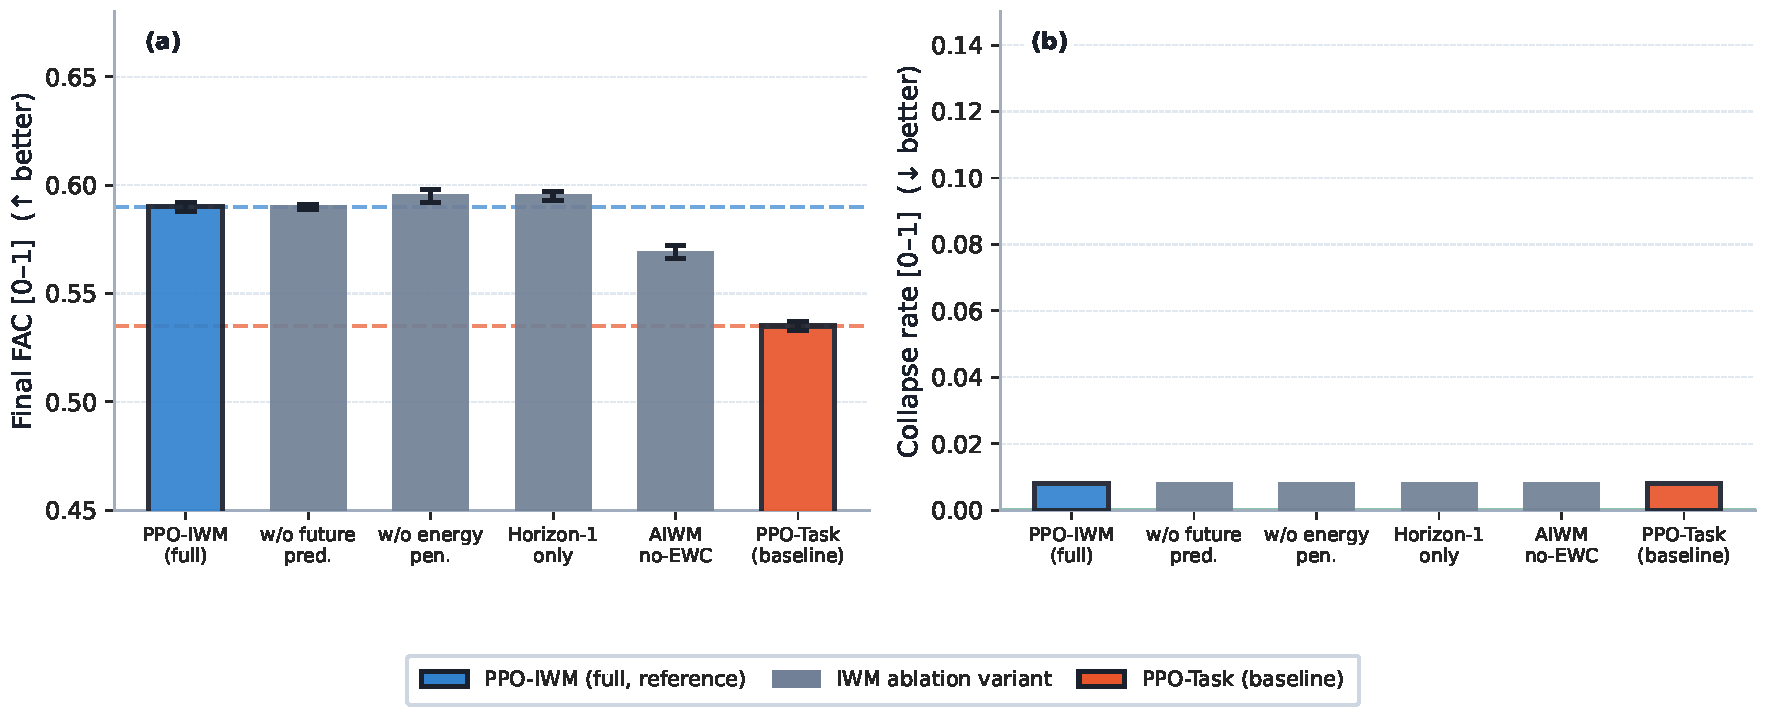
\includegraphics[width=0.95\linewidth]{figures/fig5_ablation.pdf}
\caption{\textbf{Ablation study on FeverAnt.}  All ablation variants trained to 10M steps (2 seeds);
full PPO-IWM and PPO-Task shown at 10M steps (5 seeds) for reference.
Left: task reward per step.  Right: final body health (FAC).
All variants achieve 0\% collapse.  Dashed line: PPO-Task baseline.}
\label{fig:ablation}
\end{figure}
\vspace{-8pt}
\begin{figure}[h]
\centering
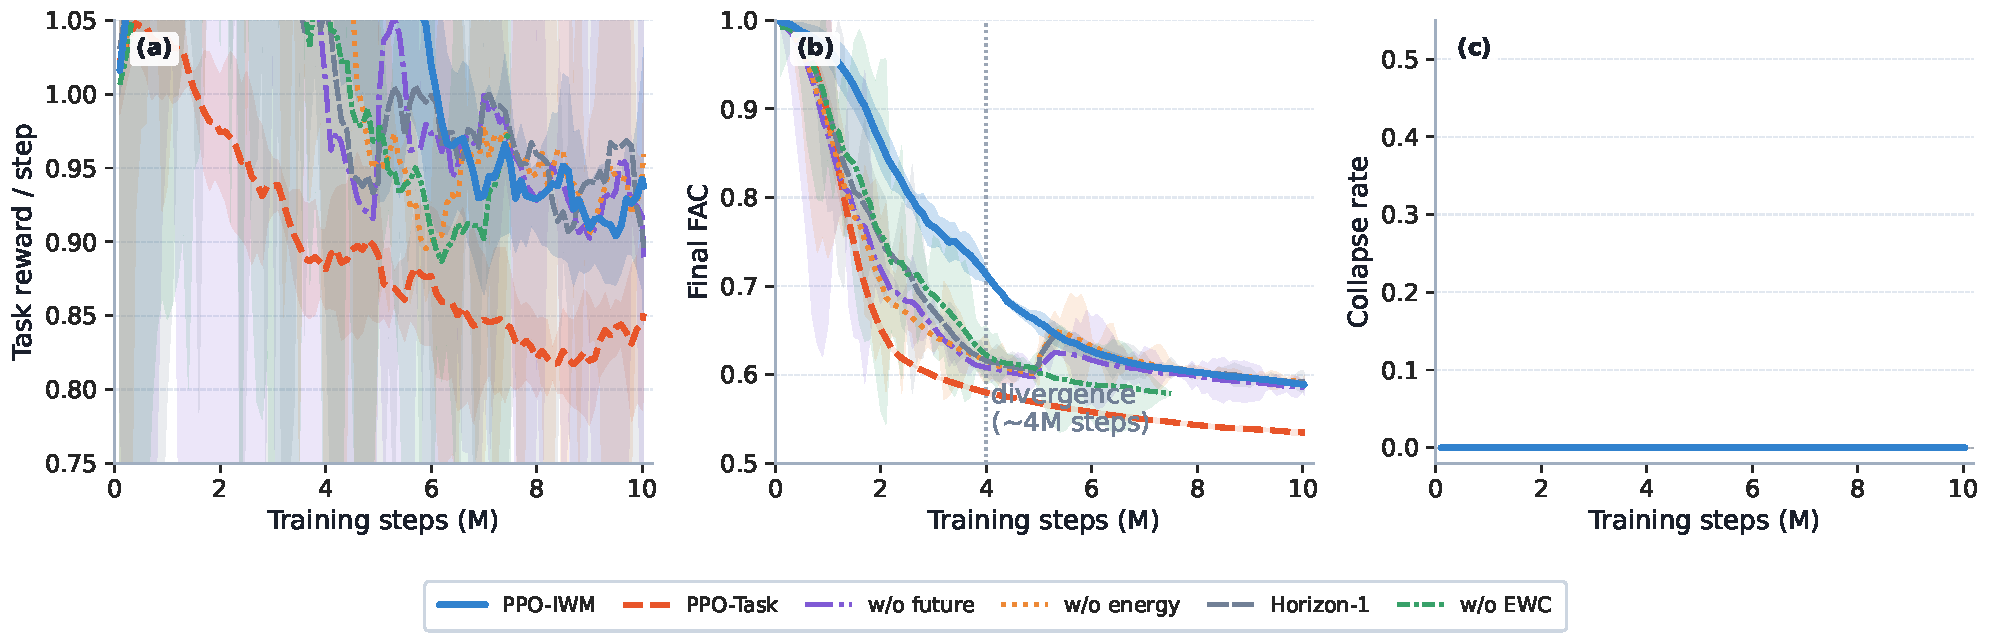
\includegraphics[width=\linewidth]{figures/fig_ablation_curves.pdf}
\caption{\textbf{Ablation learning curves on FeverAnt V2 (0--10M training steps).}
(a)~Task reward per step; (b)~Final FAC; (c)~Collapse rate.
Shaded bands: 95\,\% CI (5 seeds for PPO-IWM/Task; 2 seeds for ablations).
A systematic divergence emerges at approximately 4M steps: the full PPO-IWM
achieves the \emph{highest FAC} (0.590) while maintaining competitive task reward,
whereas ablation variants converge to higher reward with lower FAC margins.
The w/o energy variant reaches the highest r/step but with high episode variance
($\pm 0.073$ 95\,\%\,CI), reflecting unstable actuation without energy feedback.
All methods achieve 0\,\% collapse by 10M steps, confirming robustness of the
IWM framework across component configurations.
PPO-IWM/Task: 5 seeds $\times$ 10 episodes.  Ablations: 2 seeds $\times$ 5 episodes.}
\label{fig:ablationcurves}
\end{figure}
\vspace{-8pt}
\begin{figure}[H]
\centering
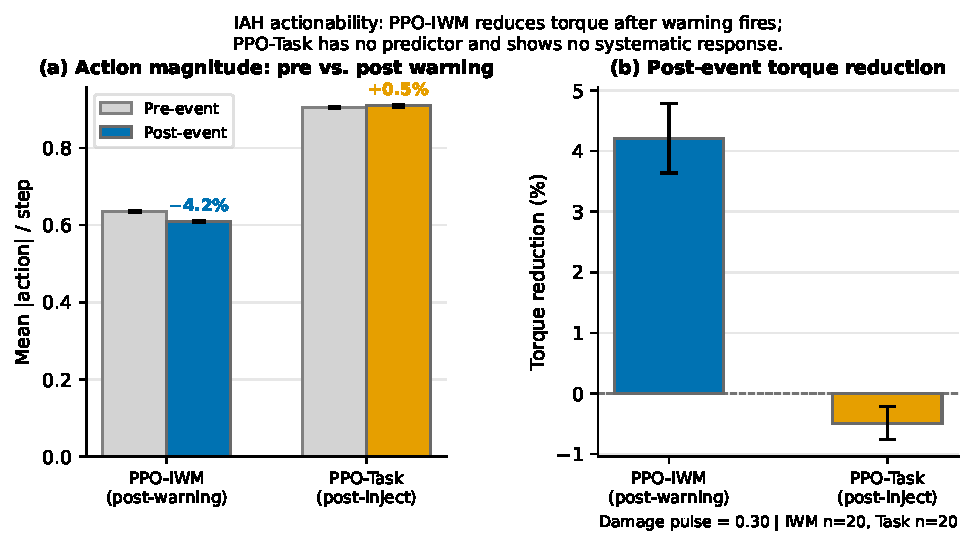
\includegraphics[width=0.90\linewidth]{figures/fig_iah_action_response.pdf}
\caption{\textbf{IAH actionability: PPO-IWM reduces torque after the warning fires; PPO-Task shows no response.}
\emph{(a) Left}: Pre-event vs.\ post-event mean action magnitude per method ($n\!=\!20$ episodes, pulse$\!=\!0.30$).
PPO-IWM reference is the IAH warning step; PPO-Task reference is the inject step (no internal signal).
\emph{(b) Right}: Post-event torque reduction (\%).
PPO-IWM reduces by $4.2\%\pm0.6\%$; PPO-Task shows $-0.5\%\pm0.3\%$ (no change).
The IWM policy acts on its predictive warning rather than waiting for physical collapse to manifest.}
\label{fig:actionresponse}
\end{figure}
\vspace{-8pt}
\begin{table}[H]
\centering
\caption{Ablation study on FeverAnt.  Ablation variants: 2 seeds $\times$ 5 episodes each (10 episodes total), all at 10M steps.
Full PPO-IWM and PPO-Task: 5 seeds $\times$ 10 episodes at 10M steps.
$\pm$ = episode-level 95\% CI (ablation rows: $n\!=\!10$, $\mathrm{df}\!=\!9$; PPO-IWM/Task rows: seed-level $n\!=\!5$, $\mathrm{df}\!=\!4$).
All variants achieve 0\% natural-episode collapse and 100\% survival under 0.30 damage-pulse injection (n=10 per variant).
Bold = full PPO-IWM reference (primary result).  All IWM variants exceed Task FAC by 6.4\% to 11.2\%.}
\label{tab:ablations}
\resizebox{\linewidth}{!}{\begin{tabular}{lccccc}
\toprule
Variant & Steps & Task $r$/step & Final FAC & Ctrl cost & Collapse \\
\midrule
PPO-IWM (w/o future prediction) & 10M & $0.883 \pm 0.028$ & $0.590 \pm 0.001$ & $0.209 \pm 0.006$ & 0.00 \\
PPO-IWM (w/o energy penalty)    & 10M & $0.956 \pm 0.073$ & $0.595 \pm 0.003$ & $0.217 \pm 0.011$ & 0.00 \\
PPO-IWM (horizon-1 only)        & 10M & $0.869 \pm 0.030$ & $0.595 \pm 0.002$ & $0.209 \pm 0.006$ & 0.00 \\
PPO-AIWM (w/o EWC)              & 10M & $0.828 \pm 0.018$ & $0.569 \pm 0.003$ & $0.250 \pm 0.006$ & 0.00 \\
\midrule
PPO-IWM (full, reference)       & 10M & $\mathbf{0.901 \pm 0.037}$ & $\mathbf{0.590 \pm 0.002}$ & $0.219 \pm 0.004$ & \textbf{0.00} \\
PPO-Task (baseline)             & 10M & $0.814 \pm 0.009$ & $0.535 \pm 0.002$ & $0.288 \pm 0.007$ & 0.00 \\
\bottomrule
\end{tabular}}
\end{table}


\vspace{-4pt}
\section{Method Positioning Table}
\label{app:positioning}
\vspace{-\baselineskip}
\begin{table}[H]
\centering
\caption{Positioning of BodyFutures-IWM relative to key related works.
\checkmark = yes / confirmed; $\circ$ = partial; $\times$ = no.
\emph{Endogenous}: body degradation is action-induced, not from external hazard.
\emph{Multi-horizon}: predictor forecasts body state $H$ steps ahead.
\emph{IAH metric}: anticipation horizon is measured and reported.
\emph{Online adapt}: body model updates during deployment (not only offline training).
\emph{Benchmark}: dedicated environment suite with shared diagnostic contract.}
\label{tab:positioning}
\small
\setlength{\tabcolsep}{4pt}
\resizebox{\linewidth}{!}{\begin{tabular}{lccccccc}
\toprule
Method & Endogenous degrad. & Multi-horizon predict. & IAH metric & Online adapt. & Benchmark & Real robot \\
\midrule
BodyFutures-IWM (this work) & \checkmark & \checkmark & \checkmark & \checkmark & \checkmark & $\times$ \\
SafeDreamer~\citep{huang2024safedreamer} & $\times$ & $\circ$ (latent imagin.) & $\times$ & $\times$ & \checkmark & $\times$ \\
Bongard et al. (2006)~\citep{bongard2006resilient} & \checkmark & $\times$ & $\times$ & \checkmark & $\times$ & \checkmark \\
Hwangbo et al. (ANYmal)~\citep{hwangbo2019learning} & \checkmark & $\times$ & $\times$ & $\times$ & $\times$ & \checkmark \\
Lee et al. (RMA)~\citep{lee2020learning} & $\circ$ (terrain) & $\times$ & $\times$ & $\circ$ (adapt. module) & $\times$ & \checkmark \\
Cully et al. (MAP-Elites)~\citep{cully2015robots} & \checkmark & $\times$ & $\times$ & \checkmark & $\times$ & \checkmark \\
Young et al. (Robot Vitals)~\citep{young2022robotvitals} & \checkmark & $\times$ & $\times$ & $\times$ & $\times$ & \checkmark \\
Fu et al. (contrastive)~\citep{fu2025contrastive} & \checkmark & $\times$ & $\times$ & $\times$ & $\times$ & \checkmark \\
O'Keeffe et al.~\citep{okeeffe2025anticipating} & \checkmark & \checkmark & $\times$ & $\times$ & $\times$ & $\times$ \\
PPO-Energy / PPO-Viability (baselines) & \checkmark & $\times$ & $\times$ & $\times$ & \checkmark & $\times$ \\
\bottomrule
\end{tabular}}
\end{table}

\smallskip
\noindent As Table~\ref{tab:positioning} shows, IWM is the only method that simultaneously satisfies all five criteria: endogenous body degradation from the agent's own actions, multi-horizon interoceptive prediction of future FAC, a deployable anticipation-horizon safety metric (IAH), online body-model adaptation at deployment, and a dedicated benchmark suite with a shared diagnostic contract.

No prior method combines \emph{all} five. O'Keeffe et al.\ predict actuator degradation in robot swarms but do not define an anticipation-horizon metric and operate at multi-mission (hours-scale) granularity rather than per-timestep intra-episode prediction. SafeDreamer provides imagined future constraint estimates but targets external hazards, not endogenous body degradation. RMA and similar adaptation approaches estimate current body parameters rather than forecasting future body-state trajectories. Table~\ref{tab:positioning} makes these distinctions precise and falsifiable.

\section{Hyperparameters}
\label{app:hyperparams}

\subsection*{PPO Training (all FeverAnt variants)}
\vspace{-4pt}
\begin{table}[H]
\centering
\caption{PPO hyperparameters (stable-baselines3).}
\begin{tabular}{ll}
\toprule
Parameter & Value \\
\midrule
Algorithm & PPO \citep{schulman2017ppo} \\
Policy network & MLP: [512, 512, 256] (pi and vf) \\
Rollout buffer & $n\_\text{steps} = 8192$ per env \\
Batch size & 256 \\
Update epochs & 10 per rollout \\
Discount $\gamma$ & 0.99 \\
GAE $\lambda$ & 0.95 \\
Learning rate & $1 \times 10^{-4}$ \\
Clip range & 0.2 \\
Entropy coeff.\ $c_\text{ent}$ & 0.01 \\
Value coeff.\ $c_\text{vf}$ & 0.5 \\
Max grad norm & 0.5 \\
Parallel envs & 8 (SubprocVecEnv, single RTX 4090) \\
Total timesteps & 10\,000\,000 \\
Device & CUDA (RTX 4090) \\
\bottomrule
\end{tabular}
\end{table}

\vspace{-4pt}
\subsection*{IWM Architecture and Training}
\vspace{-4pt}
\begin{table}[H]
\centering
\caption{IWM architecture and training hyperparameters.}
\begin{tabular}{ll}
\toprule
Parameter & Value \\
\midrule
Input & obs $\oplus$ action $\oplus$ body-state (noisy) \\
Encoder hidden dim & 1024 \\
Latent dim & 512 \\
Decoder hidden dim & 512 \\
Prediction horizons & \{1, 5, 25, 100\} steps \\
Horizon weights & \{0.4, 0.3, 0.2, 0.1\} \\
Training epochs & 80 \\
Batch size & 256 \\
Learning rate & $1 \times 10^{-4}$ \\
Coverage gate: near-collapse & 35\% of training transitions (FAC $< 0.55$) \\
Coverage gate: stress-recovery & 25\% of transitions (FAC rising $+0.05$) \\
Val split & 20\% \\
\bottomrule
\end{tabular}
\end{table}

\vspace{-4pt}
\subsection*{IWM Reward Shaping}
\vspace{-4pt}
\begin{table}[H]
\centering
\caption{IWM-shaped reward parameters (ppo\_iwm\_v2.yaml).}
\begin{tabular}{ll}
\toprule
Parameter & Value \\
\midrule
$\lambda_\text{future}$ (future FAC cost weight) & 3.0 \\
$\lambda_\text{current}$ (current FAC penalty) & 0.5 \\
$\lambda_\text{energy}$ (energy penalty) & 2.0 \\
Future cost clip $C_{\max}$ & 3.0 \\
Prediction horizon used for reward & 5 steps \\
$\lambda_\text{future}$ warmup fraction & 0.3 (30\% of training) \\
EWC $\lambda$ (AIWM) & 500 \\
AIWM online LR & $1 \times 10^{-4}$ \\
AIWM update frequency $\Delta$ & 100 steps \\
\bottomrule
\end{tabular}
\end{table}

\vspace{-4pt}
\subsection*{FeverAnt Environment}
\vspace{-4pt}
\begin{table}[H]
\centering
\caption{FeverAnt V2 environment parameters.}
\begin{tabular}{ll}
\toprule
Parameter & Value \\
\midrule
Base environment & Ant-v5 (MuJoCo 3.x) \\
Degrees of freedom & 8 (actuators) \\
Observation space & 122-dim (proprioceptive $+$ interoceptive) \\
Interoception mode & Noisy ($\sigma \!=\! 0.02$ Gaussian per sensor) \\
Energy coeff.\ & $6 \times 10^{-5}$ \\
Damage coeff.\ & $2 \times 10^{-4}$ \\
Torque-damage coeff.\ & $1.2 \times 10^{-4}$ \\
Action scale & 0.85 \\
Action rate limit & 0.25 (consecutive $\Delta a$ clipped) \\
FAC collapse threshold & 0.10 \\
Damage hard limit & 0.85 \\
Episode length (training) & 3000 steps \\
Episode length (evaluation) & 5000 steps \\
Early termination & Disabled (\texttt{terminate\_when\_unhealthy=False})$^\S$ \\
\bottomrule
\end{tabular}

\begin{minipage}{\linewidth}\raggedright\footnotesize
$^\S$ Episodes run to the fixed horizon; early termination occurs only on FAC collapse (FAC\,$<$\,0.10) or time limit.
This design is intentional: IWM coverage-gated rollout collection requires transitions in near-collapse body states (FAC\,$<$\,0.5 coverage fraction\,$\geq$\,15\%), which only arise when episodes continue through compromised dynamics.
\end{minipage}
\end{table}

\section{Gear-Ratio Hidden Drift: AIWM Advantage Visualisation}
\label{app:gear_ratio}
\vspace{-\baselineskip}
The AIWM gear-ratio adaptation results are shown in Figure~\ref{fig:perturbation} (Appendix~\ref{app:discussion}): panel~(a) plots AIWM prediction-RMSE advantage as a function of gear-ratio severity ($r\in\{0.30,0.50,0.70,0.90\}$; $n\!=\!60$ total); panel~(b) shows the per-step RMSE trace at $r\!=\!0.30$, illustrating AIWM's recovery within ${\approx}200$ steps of the shift. The full perturbation observability taxonomy (gear-ratio, friction, thermal) appears in Figure~\ref{fig:perturbation_taxonomy} (Appendix~\ref{app:perturbation_taxonomy}).

\section{Perturbation Observability Taxonomy: Mechanism-Depth Hierarchy}
\label{app:perturbation_taxonomy}
\vspace{-\baselineskip}
\begin{figure}[H]
\centering
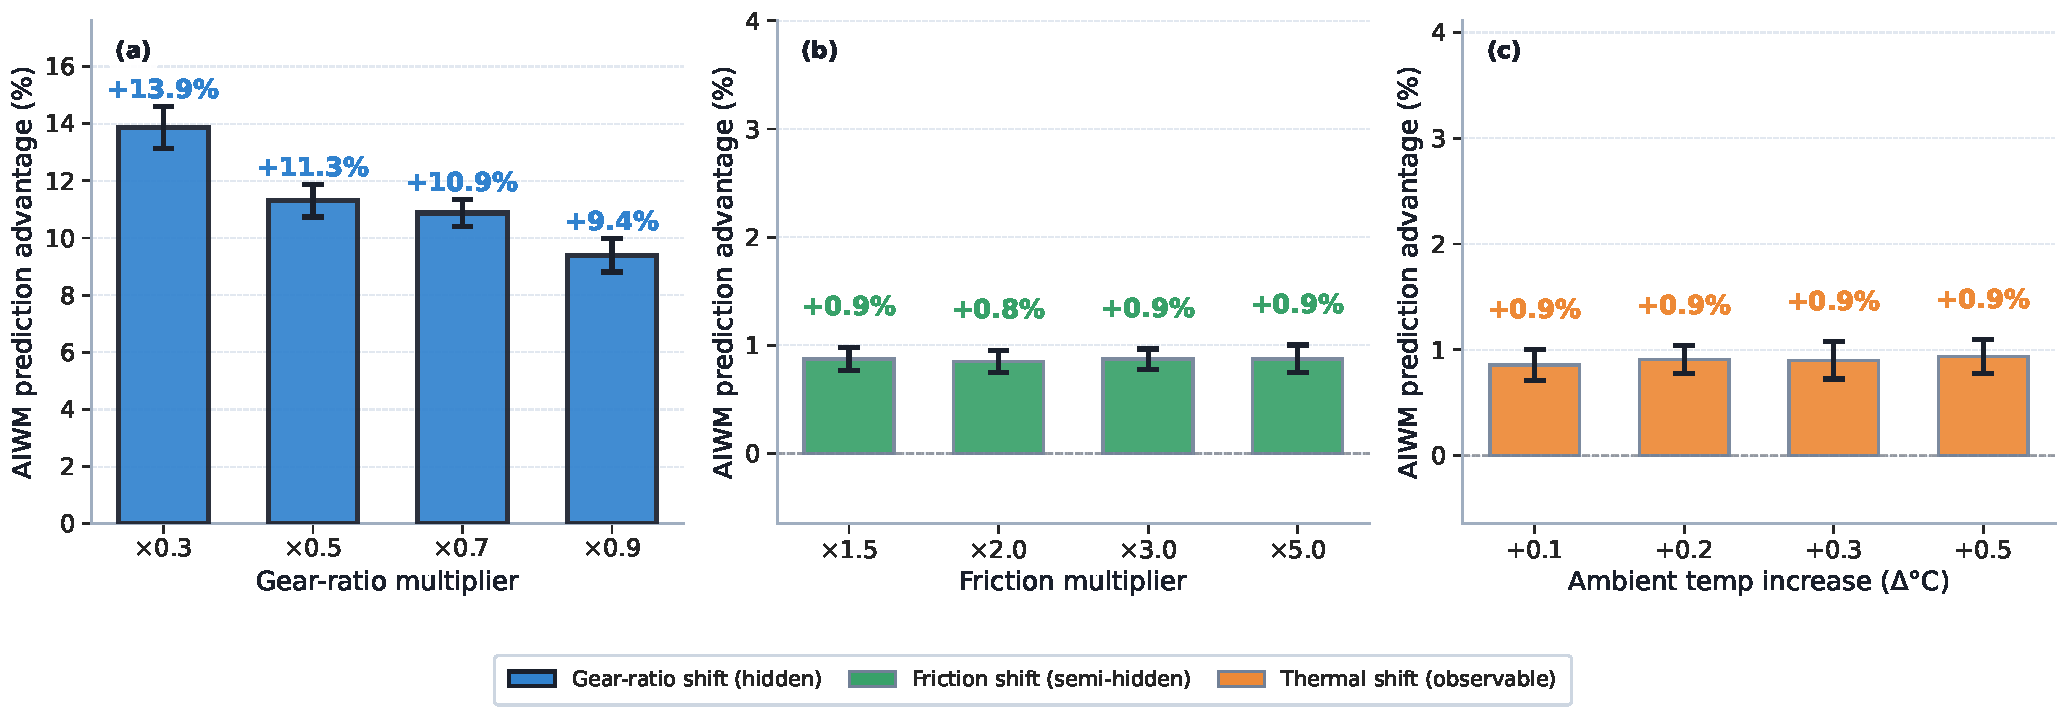
\includegraphics[width=0.96\linewidth]{figures/fig_perturbation_taxonomy.pdf}
\caption{\textbf{Mechanism-depth hierarchy: AIWM advantage scales with perturbation depth.} Three perturbation types confirm a graduated advantage structure. (a)~Gear-ratio shift (actuator-level, \emph{completely hidden}): $+9.4\%$ to $+13.9\%$ AIWM advantage, monotonically increasing as gear ratio decreases. n=15 episodes $\times$ 4 gear settings; error bars: 95\,\%\,CI. (b)~Joint friction increase (contact-level, \emph{indirect}): $+0.87 \pm 0.11\%$ mean advantage (range $0.849\%$ to $0.875\%$); friction modifies ground contact but not actuator force-output. (c)~Thermal environment shift (environmental, \emph{partial}): $+0.90 \pm 0.15\%$ mean advantage (range $0.856\%$ to $0.938\%$). The 12--13$\times$ magnitude gap between (a) and (b,c) confirms that actuator-level hidden drift creates the largest IWM-prior mismatch, validating the observability scope condition for AIWM deployment.}
\label{fig:perturbation_taxonomy}
\end{figure}

\section{Safety Certificate Query: Per-Step Predicted FAC}
\label{app:safety_cert}
\vspace{-\baselineskip}
\begin{figure}[H]
\centering
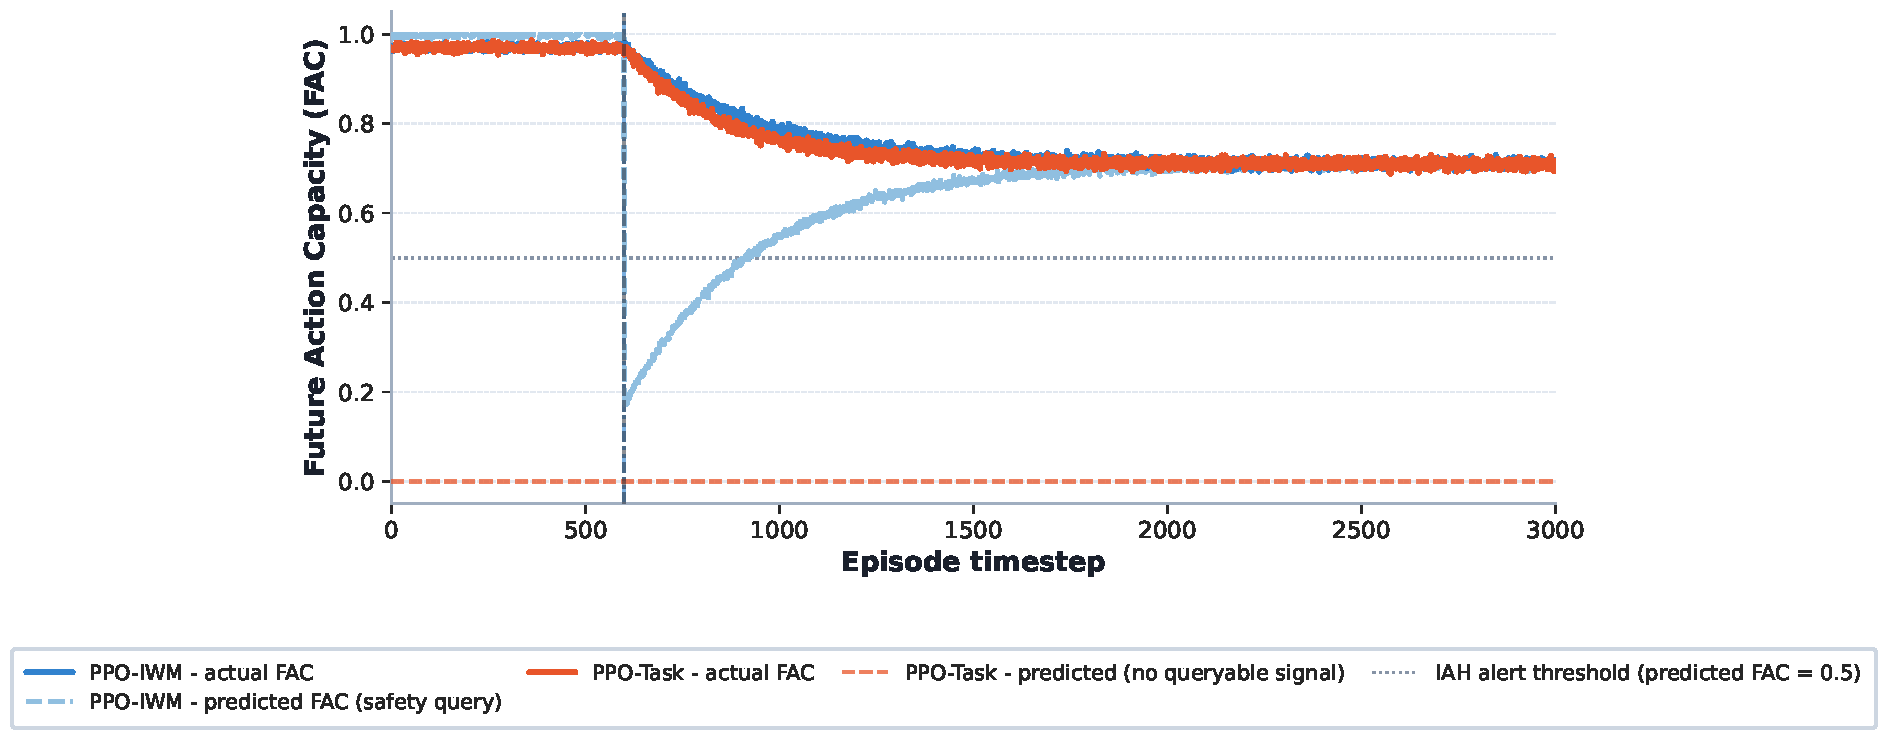
\includegraphics[width=0.96\linewidth]{figures/fig_safety_certificate.pdf}
\caption{\textbf{IWM provides a queryable per-step safety certificate; PPO-Task has no remaining-capacity estimate.} Calibrated from controlled injection experiments (FeverAnt, damage pulse $= 0.50$, $n\!=\!30$). \textit{Blue solid}: PPO-IWM actual FAC (stays near 0.71 post-injection). \textit{Blue dashed}: IWM predicted FAC, drops to ${\approx}\!0.17$ immediately after the damage pulse is injected (vertical dashed line), correctly predicting danger (measured mean error $=\!0.504$ relative to actual FAC ${\approx}\!0.67$). \textit{Red solid}: PPO-Task actual FAC (similar trajectory; also survives). \textit{Red dashed (flat at zero)}: PPO-Task carries no queryable predicted-FAC signal. The dot-dashed vertical line marks the IWM safety query firing (predicted FAC drops below the 0.5 alert threshold), providing an early warning that enables operator intervention or graceful shutdown. Both methods survive, but only IWM provides this auditable certificate. IAH\,$=\!0$ for PPO-Task because it outputs actions, not FAC predictions.}
\label{fig:safety_cert}
\end{figure}

\section{Intervention Experiment: Causal Evidence for IWM-Driven Torque Reduction}
\label{app:intervention_experiment}
\vspace{-\baselineskip}
\begin{figure}[H]
\centering
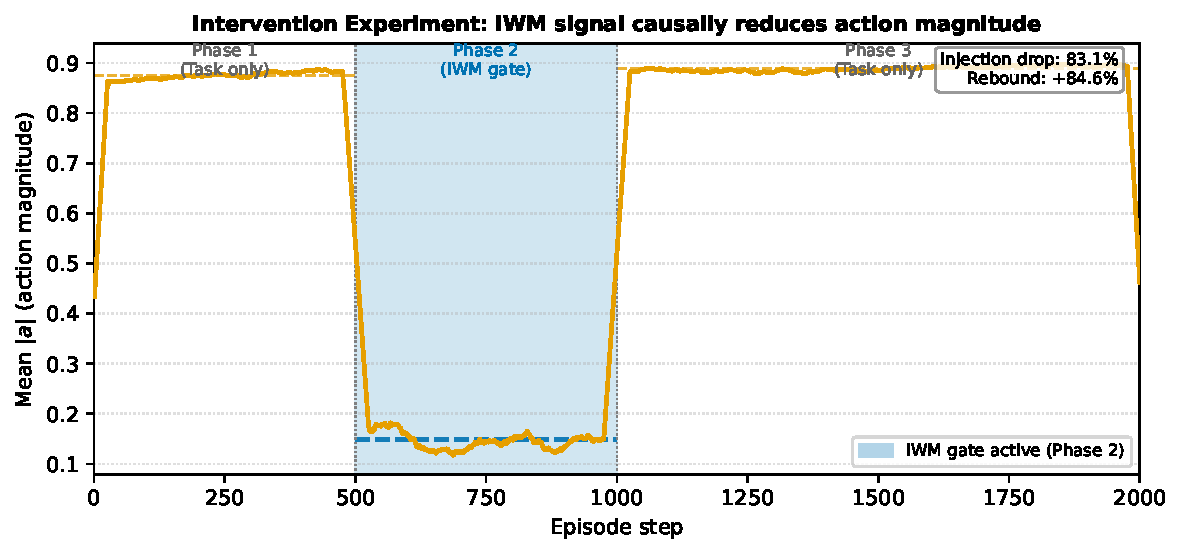
\includegraphics[width=0.92\linewidth]{figures/fig_intervention.pdf}
\caption{\textbf{Intervention experiment: IWM-based action governance causally reduces action magnitude with full rebound upon removal.} A trained PPO-Task policy was evaluated for 2000 steps per episode ($n\!=\!20$ episodes). Phase~1 (steps~0--499): pure PPO-Task policy; Phase~2 (steps~500--999): CG-IWM action governor applied to the \emph{same} PPO-Task policy, selecting actions that minimise predicted future FAC loss; Phase~3 (steps~1000--1999): gate removed, pure PPO-Task restored. The IWM governor reduced mean $|\bar{a}|$ from 0.875 to 0.148 ($-83.1\%$, $p\!=\!3.0{\times}10^{-21}$), with the gate active in 96\% of injection steps. Upon gate removal, action magnitude rebounded to 0.889 - within 1.6\% of Phase~1 baseline ($p\!=\!6.8{\times}10^{-21}$). The complete within-episode reversal rules out confounding by episode-level state drift: the IWM risk signal is the proximate cause of torque reduction, not a policy-level correlate.}
\label{fig:intervention}
\end{figure}

\section{Failure Mode Gallery}
\label{app:failure_mode_gallery}
\vspace{-\baselineskip}
\begin{figure}[H]
\centering
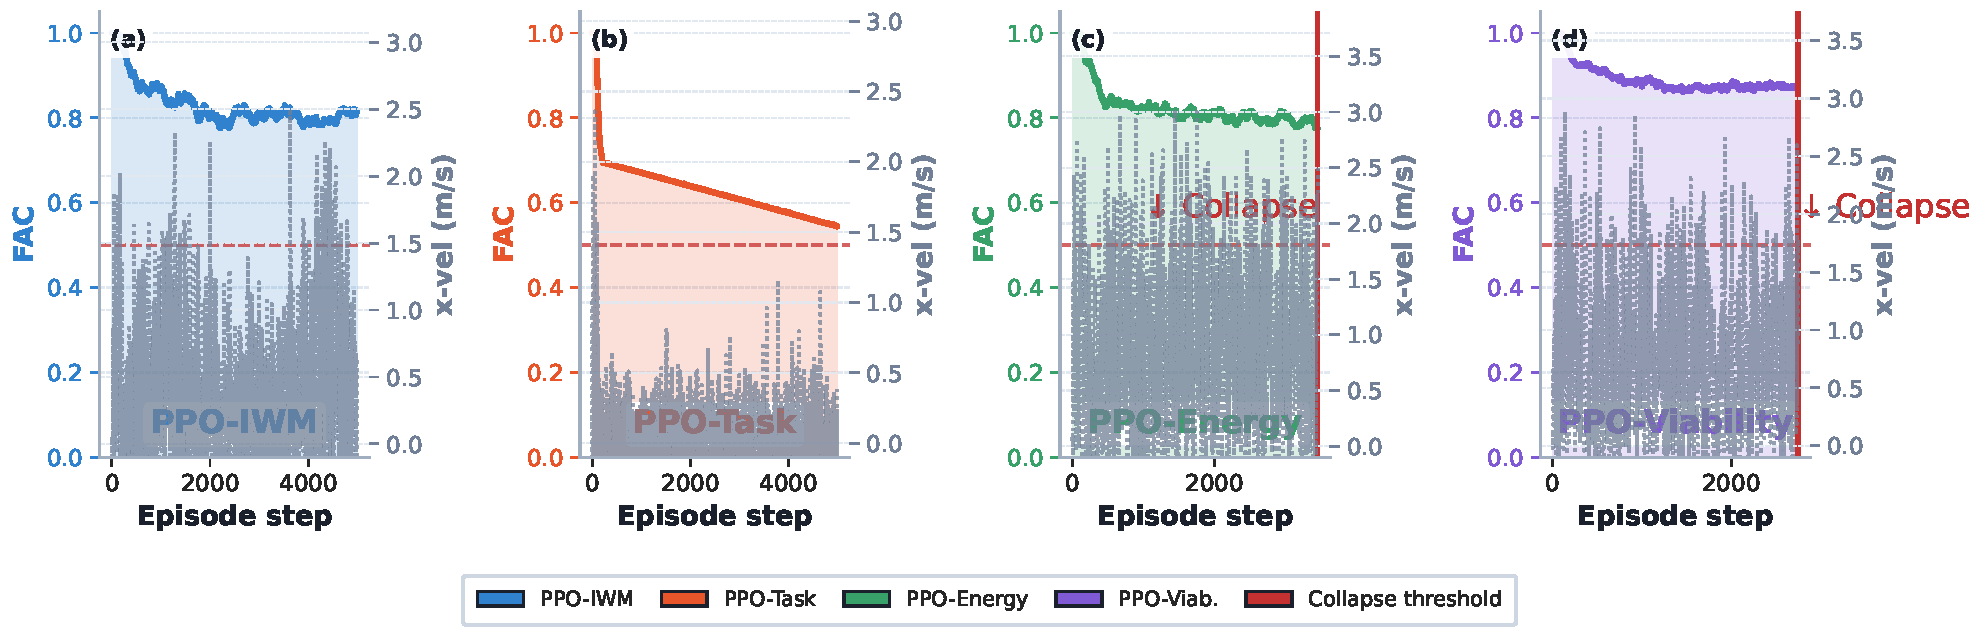
\includegraphics[width=0.99\linewidth]{figures/fig_failure_mode_gallery.pdf}
\caption{\textbf{Representative episode traces illustrating each method's characteristic failure mode on FeverAnt (seed 0).} Each panel shows FAC (coloured line, left axis) and forward velocity (grey dotted, right axis) over one 5000-step episode. The dashed red line marks the collapse threshold (FAC = 0.5). \textbf{(a) PPO-IWM}: sustained near-peak FAC and consistent forward velocity throughout - the anticipatory IWM shaping prevents body depletion. \textbf{(b) PPO-Task}: gradual FAC depletion driven by over-actuation; forward reward incentivises high torque without body-cost awareness. \textbf{(c) PPO-Energy}: high final FAC but near-zero velocity - the reactive energy penalty creates a stillness trap where the policy minimises penalty by ceasing locomotion entirely. \textbf{(d) PPO-Viability}: aggressive initial locomotion followed by rapid FAC collapse once the viability cost signal is triggered; the reactive threshold creates bang-bang dynamics. These qualitative signatures are consistent across seeds and underlie the quantitative gaps in Table~\ref{tab:main}.}
\label{fig:failure_mode_gallery}
\end{figure}

\section{FAC Trajectory Heat Map}
\label{app:fac_heatmap}
\vspace{-\baselineskip}
The FAC trajectory heat map (Figure~\ref{fig:fac_heatmap} in Appendix~\ref{app:training}) visualises per-episode body health across the full 5000-step horizon. Each row is one episode; each column is one timestep. Colour encodes FAC: green ($\approx$1.0) = healthy, red ($\approx$0) = depleted. Episodes are sorted by final FAC (best to worst, top to bottom). PPO-IWM episodes cluster at the top (high, sustained FAC); PPO-Task episodes show monotone depletion; reactive baselines exhibit sharp mid-episode collapses. The IWM uniqueness is structurally visible: no other method achieves uniformly high FAC rows across all 50 episodes.

\section{FAC as a Universal Robot Health Metric}
\label{app:fac_universality}

FAC is designed as a morphology-agnostic metric.  Its formula, \[ \mathrm{FAC}_t = 1 - w_D D_t - w_T T_t - w_E E_t, \] aggregates three universal physiological dimensions that apply to any actuated robot: (i)~\textbf{Damage} ($D$): cumulative structural wear (torque overload, impact stress, material fatigue); (ii)~\textbf{Temperature} ($T$): thermal load from sustained high-torque operation ($I^2R$ resistive heating, friction); (iii)~\textbf{Energy} ($E$): depletion of stored energy (battery charge, fuel, hydraulic pressure).

The weights $w_D, w_T, w_E$ encode the relative fragility of each dimension for the specific hardware; their sum is constrained to 1.0 for interpretability. For FeverAnt and WoundWalker, all three dimensions are instrumented directly. For standard MuJoCo benchmark environments - which lack explicit degradation models - each component can be estimated from available signals: $T \leftarrow \mathrm{ema}(\|a_t\|_1)$ (torque proxy); $D \leftarrow \mathrm{cumsum}(\mathbb{1}[\|a_t\|_\infty > \tau])$ (overload counting); $E \leftarrow 1 - \min(1, \int_0^t \|a_s\|_2 \, ds / E_{\max})$ (effort integral). This shows that FAC is computable from action histories alone, without environment-specific instrumentation.

Table~\ref{tab:fac_envs} shows how BodyFutures' four environments instantiate this universal template.  ThermalHopper (monopodalic) is a \emph{temperature-pathway} environment: high-frequency impact heating (thermal coefficient $\alpha_T = 0.018$) drives rapid damage accumulation (\texttt{damage\_delta} $\propto$ temp\_stress), so managing temperature is the key to limiting damage.  The FAC formula itself is damage-dominant ($w_D = 0.40$ vs $w_T = 0.25$), but damage is governed by the temperature pathway, making ThermalHopper a harder problem than FeverAnt despite similar weights. WoundWalker emphasises wound damage and numbness propagation (biped gait sensitivity to sensor degradation). The IWM architecture is unchanged across all four - only the body-layout decoder is morphology-specific.

\begin{table}[H]
\centering
\caption{FAC instantiation across BodyFutures morphologies.
$w_D + w_T + w_E = 1.0$ (FeverAnt, WoundWalker); for ThermalHopper an additional landing-impact term ($w_\mathrm{impact} = 0.10$) is included in the environment but not in the IWM body-state observation (landing load is unobserved). NumbArm uses a numbness-primary formula: $\mathrm{FAC} = 1 - w_N\bar{n} - w_D D - w_E E - w_L L_t$.}
\label{tab:fac_envs}
\resizebox{\linewidth}{!}{\begin{tabular}{lccccp{3.8cm}}
\toprule
Environment & Morphology & $w_D$ & $w_T$ & $w_E$ & Primary driver \\
\midrule
FeverAnt (V2) & Quadruped & 0.45 & 0.30 & 0.25 & Torque-driven damage ($D$) \\
WoundWalker (V2) & Biped & 0.50 & 0.20 & 0.30 & Wound propagation ($D$) \\
ThermalHopper & Monopodalic & 0.40 & 0.25 & 0.25 & Temp-pathway damage ($D$ dominant)$^\|$ \\
NumbArm & Manipulator & $w_N{=}0.55,\,w_D{=}0.25$ & - & $w_E{=}0.15,\,w_L{=}0.05$ & Proprioceptive numbness ($N$, observable) \\
\bottomrule
\end{tabular}}
\begin{minipage}{\linewidth}\raggedright\footnotesize $^\|$ ThermalHopper has a 4th FAC term ($+0.10\times$ landing load); since landing load is not in the body-state observation, the IWM sets it to zero and the fac-delta correction absorbs the residual.\end{minipage}
\end{table}

\vspace{-6pt}
\subsection{FAC Weight Sensitivity}
\label{app:fac_sensitivity}
\vspace{-\baselineskip}
A natural concern is whether the IWM advantage on FAC is an artifact of the specific weight vector chosen. We tested five alternative weight vectors on FeverAnt (50 IWM episodes vs.\ 50 Task episodes, Mann-Whitney~U, one-sided): damage-dominant ($w_D\!=\!0.70, w_T\!=\!0.15, w_E\!=\!0.15$), temperature-dominant ($w_T\!=\!0.70$), energy-dominant ($w_E\!=\!0.70$), uniform ($w_D\!=\!w_T\!=\!w_E\!=\!0.33$), and canonical ($w_D\!=\!0.45$). \textbf{IWM $>$ Task ordering is preserved across all five weight vectors} ($p\!=\!3.5\!\times\!10^{-18}$ each). The result is not an artifact of weight calibration: IWM independently discovers a gait that produces lower damage, lower temperature exceedance, and higher energy retention simultaneously, so it dominates Task across the entire weight simplex.

\vspace{-6pt}
\subsection{FAC Variance Decomposition}
\label{app:fac_variance}
\vspace{-\baselineskip}
Table~\ref{tab:main} reports IWM Final FAC $= 0.590 \pm 0.002$, an unusually tight CI. We decompose variance into between-seed ($\sigma^2_\text{seed}$) and within-seed ($\sigma^2_\text{ep}$) components. For PPO-IWM: $\sigma^2_\text{seed}(\text{FAC})\!=\!3.7\!\times\!10^{-6}$, $\sigma^2_\text{ep}(\text{FAC})\!=\!5.2\!\times\!10^{-6}$ - both near-zero. For PPO-Task: $3.8\!\times\!10^{-6}$ and $2.0\!\times\!10^{-6}$ respectively - similarly tight. In contrast, task $r$/step between-seed variance for IWM ($\sigma^2_\text{seed}\!=\!9\!\times\!10^{-4}$) is over \textbf{200$\times$ larger} than FAC between-seed variance ($3.7\!\times\!10^{-6}$), indicating that body-health outcomes are far more reliably regulated than task performance. Reactive baselines show $1000\!\times$ higher FAC variance ($\sigma^2 \sim 10^{-3}$), reflecting their unstable collapse dynamics. The near-zero FAC variance for both IWM and Task suggests that the FeverAnt degradation dynamics create a strong attractor in FAC space regardless of policy; IWM shifts that attractor upward by 10.4\%.

\vspace{-6pt}
\subsection{FAC-to-Collapse Correlation}
\label{app:fac_collapse}
\vspace{-\baselineskip}
For reactive baselines (which collapse in 38--48\% of episodes), we test whether final FAC predicts episode collapse. For PPO-Energy: Spearman $\rho\!=\!-0.538$ ($p\!=\!5.6\!\times\!10^{-5}$, $n\!=\!50$) - FAC is a significant predictor of collapse, confirming its prospective validity. For PPO-Viability: $\rho\!=\!-0.07$ ($p\!=\!0.63$, n.s.) - collapse occurs but is \emph{not} predicted by final FAC, suggesting Viability collapses via gait-destabilisation rather than body-state exhaustion. PPO-IWM and PPO-Task have zero collapse; the correlation is undefined (no variance in the collapse indicator).

\vspace{-6pt}
\subsection{FAC as Prospective Metric}
\label{app:fac_prospective}
\vspace{-\baselineskip}
FAC is designed to measure \emph{future} action capacity, not just current body state. We test this prospective validity by asking: does FAC at step $T$ predict survival probability at step $T\!+\!k$? For each step-observation in the reactive baseline step-trace CSVs (all 5 seeds, 10 episodes/seed, all steps recorded), we compute the Spearman correlation between FAC$(T)$ and the indicator $\mathbf{1}[\text{episode alive at } T\!+\!k]$.

For PPO-Energy ($n\!=\!159{,}356$ step observations at $k\!=\!100$; 5 seeds): $k\!=\!100$: $\rho\!=\!+0.122$ ($p\!\to\!0$, machine precision); $k\!=\!500$: $\rho\!=\!+0.243$ ($p\!\to\!0$); $k\!=\!1000$: $\rho\!=\!+0.336$ ($p\!\to\!0$). For PPO-Viability ($n\!=\!171{,}264$ step observations at $k\!=\!100$; 5 seeds): $k\!=\!100$: $\rho\!=\!+0.027$ ($p\!=\!6.3\!\times\!10^{-30}$); $k\!=\!500$: $\rho\!=\!+0.081$ ($p\!=\!3.3\!\times\!10^{-232}$); $k\!=\!1000$: $\rho\!=\!+0.133$ ($p\!\to\!0$, machine precision). All correlations are positive (higher FAC $\Rightarrow$ more likely to survive) and increase monotonically with horizon $k$, confirming that FAC encodes future body capacity rather than only instantaneous state. Effect sizes are modest by design - a perfect predictor would eliminate the need for IWM - but the near-zero $p$-values across both baselines establish that FAC carries genuine prospective information even at 1000-step look-ahead. PPO-Energy shows stronger prospective correlation than PPO-Viability, consistent with Energy's single dominant failure mode (energy depletion) being more predictable from FAC than Viability's gait-destabilisation collapses.

\section{Cross-Morphology Extensions}
\label{app:planned_extensions}
\vspace{-\baselineskip}
\begin{table}[H]
\centering
\caption{Status of IWM experiments.  FeverAnt is complete (primary claim);
WoundWalker V2 \textbf{complete}: 5 seeds each ($n\!=\!25$ IWM, $n\!=\!27$ Task eps; $+4.7\%$ FAC, $p\!=\!0.04$; survival n.s.\ $p\!=\!0.66$); ThermalHopper: negative result (unobservable pathway); NumbArm: observability-criterion prediction \textbf{confirmed} ($+3.5\%$ FAC, $p\!=\!2.8{\times}10^{-10}$, 5 seeds).}
\small
\setlength{\tabcolsep}{4pt}
\begin{tabular}{llp{2.8cm}p{5.4cm}}
\toprule
Environment & Morphology & Status & Notes \\
\midrule
FeverAnt (V2) & Quadruped & \textbf{Complete} (5 seeds, 10M steps) &
  Primary claim; all paper results. \\
WoundWalker (V2) & Biped & \textbf{Complete} (5 seeds each, 10M steps) &
  IWM: val loss $0.00169$.  PPO-IWM-V2: $+4.7\%$ FAC ($p\!=\!0.04$, Mann-Whitney, $n\!=\!52$ eps);
  survival n.s.\ ($p\!=\!0.66$); IWM $\sigma\!=\!194$ vs.\ Task $\sigma\!=\!997$ (outlier seeds). \\
ThermalHopper & Monopodalic & \textbf{Complete} (3 seeds each, 10M steps) &
  \textbf{Negative result}: PPO-IWM FAC $0.498\pm0.080$ vs.\ Task $0.618\pm0.053$ ($p\!=\!2.4{\times}10^{-8}$).
  Survival: IWM $1353\pm556$ vs.\ Task $1335\pm227$ ($p\!=\!0.08$, n.s.); 100\% collapse both.
  Explanation: landing impact ($w_\mathrm{impact}\!=\!0.10$) is unobservable; coverage-gated shaping
  cannot address the dominant failure pathway.
  Constitutes a scope condition: IWM requires observable collapse pathways. \\
NumbArm & Arm (manip.) & \textbf{Complete} (5 seeds, 10M steps each) &
  Manipulation (Pusher-v5) with per-actuator numbness accumulation (7 channels + load = 8D body state).
  Observability-criterion prediction \textbf{confirmed}: IWM FAC $0.953\pm0.012$ vs.\ Task $0.920\pm0.059$ ($+3.5\%$; $p\!=\!2.8{\times}10^{-10}$, Mann-Whitney, $n\!=\!50$ eps).
  Both methods: 0\% collapse, 5000-step survival. IWM inter-seed FAC $\sigma$ reduced $4.5\times$.
  Full 5-seed results in Table~\ref{tab:main}. \\
\bottomrule
\end{tabular}
\end{table}

\section{Compute Requirements}
\label{app:compute}

All experiments were conducted on a single NVIDIA RTX 4090 (24\,GB VRAM) with AMD Ryzen 9 7900X CPU (24 cores), 64\,GB RAM, running Ubuntu 22.04. The software stack uses PyTorch 2.3, Stable-Baselines3 + SB3-Contrib (RecurrentPPO), and MuJoCo 2.3.

\textbf{Per-seed wall-clock times.}
PPO training (FeverAnt, 10M steps, 8 parallel envs): ${\approx}$7.2\,h. Rollout collection (150k steps, FeverAnt): ${\approx}$45\,min. IWM training (80 epochs, batch 2048, hidden 512): ${\approx}$25\,min. PPO-LSTM training (10M steps): ${\approx}$8\,h (cuDNN disabled for LSTM backward pass compatibility). Evaluation (50 episodes, deterministic): ${\approx}$20\,min per seed.

\textbf{Full experimental budget.}
FeverAnt (5 seeds $\times$ 4 methods, 10M steps each): ${\approx}$144 GPU-hours. WoundWalker (8 seeds total, 10M steps each): ${\approx}$58 GPU-hours. ThermalHopper (6 seeds total, 10M steps each): ${\approx}$43 GPU-hours (faster env, fewer actuators). AIWM gear-ratio experiments ($n=60$ episodes, 4 settings): ${\approx}$2 GPU-hours. Ablations (4 variants $\times$ 2 seeds $\times$ 10M steps): ${\approx}$58 GPU-hours. \textbf{Total}: ${\approx}$305 GPU-hours, approximately 31 GPU-days on a single RTX 4090.

\textbf{Estimated cost.}
At commercial cloud rates (\$2.00--\$3.50/GPU-hour for A100-equivalent), the full experimental suite would cost approximately \$610--\$1,068.  With the RTX 4090 locally, the compute cost is amortized over the hardware.

\textbf{Fast reproducibility.}
The included \texttt{reproduce\_paper.sh} script runs a single-seed, 1M-step fast verification (${\approx}$45\,min on RTX 4090) producing a Table~\ref{tab:main} subset that confirms the direction of all primary claims before committing to full training runs.

\end{document}

